\documentclass[12pt, a4paper, oneside, romanian]{teza-upb}

\setcounter{secnumdepth}{3}
\setcounter{tocdepth}{3}

\usepackage{babel}
\usepackage{graphicx}
\usepackage{float}  % specificatorul [H]: figuri/tabele fixate exact la locul lor, în ordine
\usepackage{pdfpages}  % inserarea Anexei 1/2 (formular de înscriere) ca pagini PDF
% \usepackage{svg}  % dezactivat: inkscape nu este disponibil ca subproces;
                    % oricum nu sunt includeri \includesvg în lucrare
\usepackage{xcolor}
\usepackage{setspace}
\usepackage[
  bookmarks,
  bookmarksopen=true,
  pdftitle={HomeForge. Platforma pentru automatizare rezidentiala si experimentare IoT},
  linktocpage]{hyperref}
\usepackage{minted}
\usepackage{csquotes}
\usepackage{xurl}
\usepackage{dirtree}
\usepackage{subcaption}
\usepackage{placeins}
\usepackage[backend=biber,style=ieee]{biblatex}
\addbibresource{referinte/referinte.bib}

\makeatletter
\pdfstringdefDisableCommands{%
  \def\numberline#1{#1.\space}%
}

\providecommand*{\toclevel@unnumberedsection}{1}
\makeatother

% Toleranță sporită pentru spargerea liniilor: evită overfull boxes la
% identificatori monospace lungi (căi de fișiere, nume de funcții).
\setlength{\emergencystretch}{4em}
\tolerance=3000
\hbadness=3000
\sloppy
\renewcommand{\UrlBreaks}{\do\/\do\.\do\:\do\_\do\-\do\?\do\=\do\&\do\#}

% Spațiere conformă cu regulamentul ETTI 2026 (Cap. 3.2.e: 1 – maxim 1.2 rânduri).
% Folosim single spacing (1.0), exact ca în template-ul oficial al facultății.
\singlespacing

\setminted{
  linenos,
  breaklines,
  fontsize=\scriptsize,
  frame=leftline,
  framesep=2mm, 
  tabsize=2,
  encoding=utf8
}

% \svgsetup{...}  % dezactivat odată cu pachetul svg

\graphicspath{{figuri/}}

\newcommand{\figura}[4][0.9\textwidth]{%
  \begin{figure}[htb]
    \centering
    \includegraphics[width=#1]{#2}
    \caption{#3}
    \label{fig:#4}
  \end{figure}
}

\newcommand{\codsursa}[4][]{%
  \paragraph{#3}
  \inputminted[#1]{#2}{#4}
}


\begin{document}

\author{Olteanu Rareș-Cristian}
\title{HomeForge. Platformă pentru automatizare rezidențială și experimentare IoT}

\facultatea{Facultatea de Electronică, Telecomunicații și Tehnologia Informației}
\tiplucrare{licență}
\domeniu{Electronică, Telecomunicații și Tehnologia Informației}
\catedra{Telecomunicații}
\campus{Leu}
\program{RST}
\titlulobtinut{Inginer}
\director{Ș.L. Dr. Ing. Laurențiu Boicescu}
\logostanga{logo/unstpb_logo.png}
\logodreapta{logo/ETTI-LOGO-A-1.png}

\submissionmonth{Iunie}
\submissionyear{2026}

% Formularul de înscriere a temei (Anexa 1/2), inserat după pagina de titlu (Cap. 3.1.b).
\anexainscriere{anexa1_tema.pdf}

% Regula ETTI 2026 (Cap. 3.2.h): numărul de pagină apare în subsol, centrat,
% și doar începând cu Introducerea. Paginile preliminare rămân fără număr.
\makeatletter
\renewcommand{\ps@plain}{\let\@mkboth\@gobbletwo
  \def\@oddhead{}\def\@evenhead{}\def\@oddfoot{}\def\@evenfoot{}}
\makeatother

\beforepreface
\listoffigures
\listoftables
\abbreviations{
  \raggedright
  ACID = Atomicity, Consistency, Isolation, Durability (atomicitate, consistență, izolare, durabilitate)\\
  AMQP = Advanced Message Queuing Protocol (protocol avansat de transport al mesajelor)\\
  API = Application Programming Interface (interfață de programare a aplicațiilor)\\
  CLI = Command-Line Interface (interfață în linie de comandă)\\
  CoAP = Constrained Application Protocol (protocol pentru aplicații cu resurse limitate)\\
  CORS = Cross-Origin Resource Sharing (partajare a resurselor între origini diferite)\\
  CRUD = Create, Read, Update, Delete (creare, citire, actualizare, ștergere)\\
  CSRF = Cross-Site Request Forgery (falsificare a cererilor între situri)\\
  CSS = Cascading Style Sheets (foi de stil în cascadă)\\
  CTA = Call To Action (element de îndemn la acțiune)\\
  DHCP = Dynamic Host Configuration Protocol (protocol de configurare dinamică a gazdelor)\\
  DNS = Domain Name System (sistem de nume de domeniu)\\
  DNS-SD = DNS-based Service Discovery (descoperire de servicii bazată pe DNS)\\
  DOM = Document Object Model (model de obiecte al documentului)\\
  DRF = Django REST Framework (cadru de lucru pentru API-uri REST în Django)\\
  GIN = Generalized Inverted Index (index inversat generalizat)\\
  GPIO = General-Purpose Input/Output (intrare/ieșire de uz general)\\
  HTTP = HyperText Transfer Protocol (protocol de transfer al hipertextului)\\
  I2C = Inter-Integrated Circuit (magistrală serială între circuite integrate)\\
  IoT = Internet of Things (Internetul lucrurilor)\\
  IP = Internet Protocol (protocol de internet)\\
  JSON = JavaScript Object Notation (notație de obiecte JavaScript)\\
  JSONB = JSON Binary (format binar JSON în PostgreSQL)\\
  JSX = JavaScript XML (sintaxă XML în JavaScript)\\
  JWT = JSON Web Token (token web în format JSON)\\
  LAN = Local Area Network (rețea locală)\\
  MAC = Media Access Control (control al accesului la mediu, adresă fizică)\\
  MCU = Microcontroller Unit (unitate de microcontroler)\\
  mDNS = Multicast DNS (DNS prin multicast)\\
  M2M = Machine-to-Machine (comunicație mașină-la-mașină)\\
  MQTT = Message Queuing Telemetry Transport (protocol de mesagerie de tip publish/subscribe)\\
  NVS = Non-Volatile Storage (memorie nevolatilă)\\
  OASIS = Organization for the Advancement of Structured Information Standards (organizație de standardizare)\\
  OKLCH = spațiu de culoare Oklab (coordonate Lightness, Chroma, Hue)\\
  ORM = Object-Relational Mapping (mapare obiect-relațională)\\
  OTA = Over-The-Air (actualizare fără fir)\\
  PV = Photovoltaic (fotovoltaic)\\
  QoS = Quality of Service (calitatea serviciului)\\
  RBAC = Role-Based Access Control (control al accesului bazat pe roluri)\\
  RDBMS = Relational Database Management System (sistem de gestiune a bazelor de date relaționale)\\
  REST = Representational State Transfer (transfer reprezentativ al stării)\\
  RFC = Request for Comments (document de standardizare IETF)\\
  RGB = Red, Green, Blue (roșu, verde, albastru)\\
  SOC = State of Charge (stare de încărcare a bateriei)\\
  SQL = Structured Query Language (limbaj structurat de interogare)\\
  SRV = Service record (înregistrare DNS de serviciu)\\
  SSID = Service Set Identifier (identificator al rețelei Wi-Fi)\\
  TCP = Transmission Control Protocol (protocol de control al transmisiei)\\
  TLS = Transport Layer Security (securitate la nivelul de transport)\\
  UART = Universal Asynchronous Receiver-Transmitter (receptor-transmițător asincron universal)\\
  UDP = User Datagram Protocol (protocol de datagrame)\\
  UI = User Interface (interfață cu utilizatorul)\\
  URL = Uniform Resource Locator (localizator uniform de resurse)\\
  USB = Universal Serial Bus (magistrală serială universală)\\
  UUID = Universally Unique Identifier (identificator unic universal)\\
  UX = User Experience (experiența utilizatorului)\\
  VM = Virtual Machine (mașină virtuală)\\
  XSS = Cross-Site Scripting (injectare de scripturi între situri)
}
\afterpreface

% Din corpul lucrării (de la Introducere): numărul de pagină în subsol, centrat.
\makeatletter
\renewcommand{\ps@plain}{\let\@mkboth\@gobbletwo
  \def\@oddhead{}\def\@evenhead{}%
  \def\@oddfoot{\hfil\thepage\hfil}\def\@evenfoot{\@oddfoot}}
\renewcommand{\ps@topright}{\let\@mkboth\@gobbletwo
  \def\@oddhead{}\def\@evenhead{}%
  \def\@oddfoot{\hfil\thepage\hfil}\def\@evenfoot{\@oddfoot}}
\makeatother
\pagestyle{topright}

\chapter{Introducere}

\section{Context: IoT și casele inteligente}
În ultimii ani, conceptul de \textit{Internet of Things} (IoT) s-a mutat dintr-un termen de cercetare într-un fenomen care influențează direct modul în care folosim locuința. O „casă inteligentă” înseamnă, în practică, o rețea de senzori și actuatori conectați la o unitate de control care interpretează datele și execută acțiuni automate sau manuale, declanșate de utilizator. Studiul lui Alaa et al., un \textit{review} amplu al aplicațiilor Smart Home publicate până la momentul respectiv, propune o taxonomie a acestor aplicații pe domenii precum confortul rezidențial, securitatea, eficiența energetică și asistența pentru sănătate \cite{iot_smart_home_review}.

Adopția acestor tehnologii nu depinde doar de cât de avansat este hardware-ul, ci și de cât de mult au încredere utilizatorii în sistem. Marikyan et al. observă, pe baza unei meta-analize, că factorii decisivi sunt utilitatea percepută, ușurința de utilizare și îngrijorările legate de confidențialitate \cite{marikyan_smarthome_2019}. Acest lucru este relevant pentru tema lucrării de față, fiindcă explică de ce o platformă transparentă, care rulează local și pe care utilizatorul o poate inspecta, are sens chiar și atunci când există alternative comerciale.

Pe partea de comunicație, soluțiile actuale s-au mutat în mare parte de la modelul cerere-răspuns specific HTTP la o paradigmă asincronă bazată pe \textit{publish/subscribe}. Protocolul MQTT (Message Queuing Telemetry Transport) a devenit standardul \textit{de facto} pentru schimbul de mesaje între microcontrolere și server, în primul rând datorită overhead-ului redus și a faptului că un singur broker poate distribui eficient mesaje la mulți abonați \cite{mqtt_standard_iot}. În arhitectura HomeForge, MQTT joacă exact acest rol: este magistrala prin care firmware-ul ESP32 comunică cu backend-ul Django.

% FIGURĂ DE ADĂUGAT: o schemă conceptuală a unei case inteligente -
% senzori (DHT11, BMP180), actuatori (relee), un router/broker MQTT,
% serverul HomeForge și aplicația web. Sugestie: diagrama poate fi
% desenată în draw.io / Inkscape și salvată ca PDF în figuri/.
\begin{figure}[htbp]
    \centering
    % \includegraphics[width=0.85\textwidth]{figuri/conceptul_smart_home.pdf}
    \caption{Schema conceptuală a unei case inteligente integrate în HomeForge (figură de adăugat)}
    \label{fig:concept_smarthome}
\end{figure}

\section{Limitări ale soluțiilor comerciale}
Marea majoritate a produselor de pe piață (Google Nest, Amazon Alexa, Tuya, Sonoff și variațiunile lor) lucrează după un model centrat pe cloud: dispozitivul fizic trimite datele către serverele producătorului, acolo se rulează logica de automatizare și de acolo se trimit comenzile înapoi. Există trei probleme practice cu această abordare, observate sistematic în literatură \cite{vendor_lockin_iot}.

\paragraph{Latență și dependență de internet.} O comandă banală (\textit{aprinde becul din bucătărie}) presupune un drum dus-întors prin internet către serverul producătorului. Dacă rețeaua locală e instabilă sau dacă serverele furnizorului au probleme, casa „inteligentă” devine dintr-o dată surdă. La un sistem local, același mesaj traversează doar LAN-ul și ajunge la dispozitiv în câteva milisecunde.

\paragraph{Confidențialitate.} Atunci când toate datele trec prin servere terțe, utilizatorul pierde controlul asupra lor. Dorri et al. analizează tocmai aceste vulnerabilități ale arhitecturilor IoT centralizate într-un studiu de caz Smart Home, motivând prin ele propunerea lor de a folosi blockchain ca strat alternativ de securitate \cite{dorri2017privacy}. Datele acumulate (când e cineva acasă, ce dispozitive se folosesc) pot fi monetizate sau scurse într-o breșă, fără ca proprietarul să aibă vreo cale de control direct.

\paragraph{Vendor lock-in.} Producătorii folosesc protocoale închise, firmware blocat și API-uri nedocumentate pentru a împiedica integrările între ecosisteme. În momentul în care un furnizor decide să închidă serviciile cloud, dispozitivele cumpărate devin practic deșeuri electronice \cite{vendor_lockin_iot}.

Răspunsul curent al cercetării și al comunității open-source la aceste limitări este \textit{Edge Computing}: mutarea logicii și a stocării cât mai aproape de sursa datelor, ideal în rețeaua locală a utilizatorului \cite{edge_computing_iot_2020}. HomeForge se înscrie în această direcție, dar adaugă un obiectiv suplimentar pe care îl detaliez în secțiunea următoare: \textit{transparența} sistemului.

\begin{table}[htbp]
    \centering
    \caption{Cloud-centric vs. Edge: o sinteză practică}
    \label{tab:cloud_vs_edge}
    \renewcommand{\arraystretch}{1.4}
    \small
    \begin{tabular}{|p{4cm}|p{5cm}|p{5cm}|}
        \hline
        \textbf{Aspect} & \textbf{Cloud-centric} & \textbf{Edge / Local} \\ \hline
        Locul procesării & Servere externe & Server local (LAN) \\ \hline
        Dependență de internet & Critică & Aproape inexistentă \\ \hline
        Latență tipică & 50--1000 ms & sub 5 ms \\ \hline
        Proprietatea datelor & La furnizor & La utilizator \\ \hline
        Interoperabilitate & Limitată artificial & Bazată pe protocoale deschise \\ \hline
        Suprafața de atac & Globală & Limitată la LAN \\ \hline
    \end{tabular}
\end{table}

\section{Platforme open-source și nivelul de abstractizare}
În jurul ideii de control local s-a dezvoltat o comunitate amplă, iar cea mai răspândită platformă rezultată este Home Assistant. Aceasta este o soluție matură, scrisă în Python, cu mii de integrări ce permit comunicarea cu o gamă largă de dispozitive de pe piață. Pentru un utilizator final orientat exclusiv către funcționalitate, aceasta reprezintă o alegere solidă.

Dificultatea apare însă atunci când Home Assistant este analizată din perspectiva unui student sau a unui inginer interesat de mecanismele subiacente. Pentru a putea integra atâtea categorii de dispozitive, platforma a adoptat un nivel ridicat de abstractizare: orice dispozitiv este modelat ca o „entitate" cu o „stare" discretă, comunicarea internă se realizează printr-o magistrală de evenimente, iar fluxurile concrete de rețea (interlocutori, topice MQTT, structura payload-urilor JSON) sunt acoperite de un strat de interfață grafică. Pe măsură ce platforma a evoluat, configurațiile au migrat din fișiere YAML editabile către baze de date interne (directorul \texttt{.storage} din versiunile recente). Rezultatul este o platformă potrivită pentru consumatorul final, dar opacă pentru cineva interesat de modul de funcționare la nivel inferior.

Această observație constituie punctul de pornire al proiectului HomeForge. Obiectivul nu a fost replicarea funcționalităților Home Assistant, ci asigurarea transparenței end-to-end a fluxului de date, păstrând în același timp o bază de cod redusă și ușor de parcurs.

\section{Viziunea HomeForge}
HomeForge este o platformă Smart Home cu execuție locală, concepută ca instrument didactic și mediu de experimentare pentru aplicații IoT. Spre deosebire de soluțiile care abstractizează complet stiva tehnologică, platforma menține vizibile componentele subiacente: portul 1883 al brokerului Mosquitto este expus în rețeaua locală, fiecare dispozitiv are un topic MQTT documentat, iar codul backend-ului (Django + Django REST Framework) are o dimensiune care permite parcurgerea integrală a logicii într-un interval de timp rezonabil. Arhitectura se sprijină pe patru decizii principale, descrise în continuare.

\subsection{Hardware-agnostic prin MQTT}
Spre deosebire de un middleware care ar cunoaște explicit fiecare producător, HomeForge folosește MQTT ca unică magistrală de comunicație. Orice ESP32 (sau alt microcontroler) este recunoscut de platformă dacă respectă un contract minimal: publică pe topicul \texttt{homeforge/devices/\{MAC\}/state} și se abonează la \texttt{homeforge/devices/\{MAC\}/command}. Topicele și structura payload-urilor JSON sunt definite în codul firmware (\texttt{esp32\_mqtt.ino}) și, simetric, în comanda Django \texttt{mqtt\_listener} care le procesează (\texttt{mqtt\_listener.py}). Detaliile sunt tratate în Capitolul 3.

\subsection{Stocare „schema-less" peste PostgreSQL}
Datele raportate de senzori sunt eterogene: un releu transmite o valoare booleană, o stație meteorologică transmite mai mulți parametri de tip \textit{float}, un termostat raportează simultan temperatura curentă și valoarea de referință. Adăugarea unei coloane SQL distincte pentru fiecare nou câmp ar necesita migrații frecvente; soluția adoptată este stocarea stării într-o coloană JSONB denumită \texttt{current\_state} pe modelul \texttt{Device} (\texttt{models.py:96}). Relațiile structurale (utilizator, cameră, tip de dispozitiv) rămân însă strict normalizate, fiind utilizate de mecanismul de control al accesului.

\subsection{Sincronizare optimistă a interfeței}
Pe partea de frontend (Next.js + React), s-a urmărit ca utilizatorul să nu aștepte confirmarea hardware înainte ca butonul să își schimbe starea vizuală. Implementarea folosește pattern-ul \textit{optimistic update} oferit de TanStack Query: la \texttt{onMutate} se actualizează imediat cache-ul React, iar la o eventuală eroare (\texttt{onError}) se efectuează rollback la starea anterioară (\texttt{SmartDeviceCard.tsx:78-127}). Detaliile sunt tratate în Capitolul 4.

\subsection{Sandbox educațional}
Codul este menținut minimalist: backend-ul este o aplicație Django REST Framework standard, structura bazei de date poate fi inspectată prin migrațiile Django, traficul MQTT poate fi observat din linia de comandă cu \texttt{mosquitto\_sub}, iar întreaga aplicație rulează prin Docker Compose. Astfel, fluxul de la apăsarea unui buton din interfața web până la comutarea fizică a unui releu poate fi urmărit pas cu pas, fără a fi necesară traversarea unor straturi succesive de abstractizare.

\begin{figure}[htbp]
    \centering
    
\includegraphics[width=0.4\textwidth]{figuri/HomeForge_v2_color.pdf}
    \caption{Identitatea vizuală a platformei HomeForge}
    \label{fig:homeforge-logo}
\end{figure}

\section{Obiective concrete ale lucrării}
Lucrarea își propune să descrie proiectarea și implementarea HomeForge ca platformă funcțională, urmărind explicit următoarele obiective:

\textbf{Hardware și firmware embedded:}
\begin{itemize}
    \item firmware ESP32 modular care suportă cel puțin patru variante (releu simplu, termostat cu DHT11, termostat cu BMP180, variantă combinată) — vezi directorul \texttt{backend/firmware/projects/};
    \item mecanism de reconectare automată la Wi-Fi și la brokerul MQTT, cu \texttt{ClientID} bazat pe adresa MAC (\textit{watchdog} simplu, fără task-uri FreeRTOS dedicate);
    \item raportare ciclică a stării (\textit{heartbeat}) la fiecare 5 secunde, ascultare continuă pe topicul de comandă.
\end{itemize}

\textbf{Backend Django:}
\begin{itemize}
    \item API REST construit pe Django REST Framework, urmând principiile arhitecturale ale lui Fielding \cite{fielding_rest_dissertation}, cu autentificare JWT \cite{rfc_jwt} și paginare implicită;
    \item daemon MQTT integrat ca \texttt{management command} Django (\texttt{python manage.py mqtt\_listener}), care primește telemetria, o asociază cu device-ul corect prin MAC sau IP și marchează dispozitivele ca \texttt{offline} după 30 de secunde fără heartbeat;
    \item model \texttt{Device} cu o coloană \texttt{JSONField} pentru starea curentă, mapată de Django pe tipul nativ \texttt{JSONB} din PostgreSQL \cite{postgresql_jsonb_docs};
    \item sistem ierarhic de roluri (\texttt{owner}, \texttt{admin}, \texttt{user}) și un mecanism \textit{first-user-becomes-owner} aplicat la înregistrare.
\end{itemize}

\textbf{Frontend Next.js:}
\begin{itemize}
    \item dashboard cu carduri configurabile care suportă \textit{toggle}, \textit{slider} și widget-uri de sensor (temperatură, umiditate, mișcare, lumină, CO\textsubscript{2});
    \item gestionarea layout-ului prin TanStack Query, persistat pe server și cu fallback \texttt{localStorage}, suportând foldere ad-hoc de 2--4 dispozitive în stil iOS;
    \item editor vizual pentru tipuri de dispozitive (\textit{device builder}), cu propunere către administrator, aprobare/respingere și editor de firmware/wiring/documentație;
    \item vizualizare a topologiei rețelei locale folosind React Flow.
\end{itemize}

\textbf{Deployment:}
\begin{itemize}
    \item ambalare în containere Docker pentru backend, frontend și PostgreSQL (vezi \texttt{Dockerfile} și \texttt{Dockerfile});
    \item brokerul Mosquitto rulează în același container cu backend-ul, alături de Avahi pentru discovery mDNS;
    \item script unic de dezvoltare (\texttt{./dev.sh}) care pornește în paralel backend și frontend pentru dezvoltare locală fără Docker.
\end{itemize}

\section{Structura lucrării}
Lucrarea este organizată pe capitole care urmează firul natural de la teorie la implementare:
\begin{itemize}
    \item Capitolul 2 prezintă stadiul actual al tehnologiilor IoT și justifică alegerile făcute (MQTT vs. HTTP, PostgreSQL cu JSONB, stiva Next.js/React).
    \item Capitolul 3 descrie arhitectura backend-ului HomeForge: modelele de date, API-ul REST, autentificarea, daemonul MQTT și mecanismele de aprobare a tipurilor de dispozitive.
    \item Capitolul 4 detaliază aplicația web (Next.js), componentele dashboard-ului, motorul de layout, optimistic UI-ul și editorul vizual de tipuri de dispozitive.
    \item Capitolul 5 acoperă firmware-ul ESP32: protocolul de comunicație, structura proiectelor template și mecanismele de auto-detecție a dispozitivelor.
    \item Capitolul 6 documentează procesul de deployment, containerizarea și pașii de testare manuală.
    \item Capitolul 7 conține concluziile și direcții viitoare de dezvoltare.
\end{itemize}

\chapter{Stadiul actual și analiza tehnologiilor}

\section{De la HTTP la MQTT: comunicația în IoT}
La prima vedere, un microcontroler care raportează date către un server este o aplicație web ca oricare alta. În realitate, dacă încercăm să folosim HTTP/REST pentru un nod IoT, costurile devin rapid prohibitive.

Modelul cerere-răspuns presupune că senzorul deschide o conexiune TCP nouă pentru fiecare mesaj, trimite un header HTTP care, cu cookie-uri și meta-informații, poate ajunge la câteva sute de bytes, apoi așteaptă răspunsul și închide conexiunea. Atunci când serverul vrea să trimită o comandă către dispozitiv, problema se mută: HTTP nu suportă push nativ, deci fie clientul interoghează ciclic (\textit{polling}), fie se trece la WebSocket-uri, ceea ce ne aduce, de fapt, foarte aproape de paradigma de \textit{publish/subscribe}.

MQTT alege o cale diferită. Există un broker central, iar fiecare client (senzor sau aplicație) menține o singură conexiune TCP persistentă cu el. Mesajele se publică pe „topice” — șiruri ierarhice de forma \texttt{homeforge/devices/AABBCCDDEEFF/state} — iar brokerul rutează automat fiecare publicare către toți abonații topicului respectiv. Antetul minim al unui pachet MQTT este de doar 2 bytes \cite{mqtt_standard_iot}, iar protocolul oferă nativ trei niveluri de QoS și un mecanism de \textit{Last Will and Testament}, prin care brokerul detectează automat deconectarea unui nod.

Naik a evaluat comparativ patru protocoale de mesagerie pentru IoT (MQTT, CoAP, AMQP și HTTP) și a arătat că MQTT și CoAP sunt mai potrivite pentru rețele de senzori cu lățime de bandă redusă și noduri cu resurse limitate, în timp ce HTTP rămâne natural pentru integrări cu sisteme web tradiționale \cite{mqtt_vs_http_iot_perf}. Mishra și Kertész, în survey-ul lor extensiv asupra MQTT în M2M și IoT, listează implementări de broker (Mosquitto, HiveMQ, EMQ X, VerneMQ) și concluzionează că Mosquitto este una dintre cele mai populare alegeri datorită amprentei mici și a faptului că rulează inclusiv pe Raspberry Pi \cite{mqtt_standard_iot}.

\begin{figure}[htbp]
    \centering
    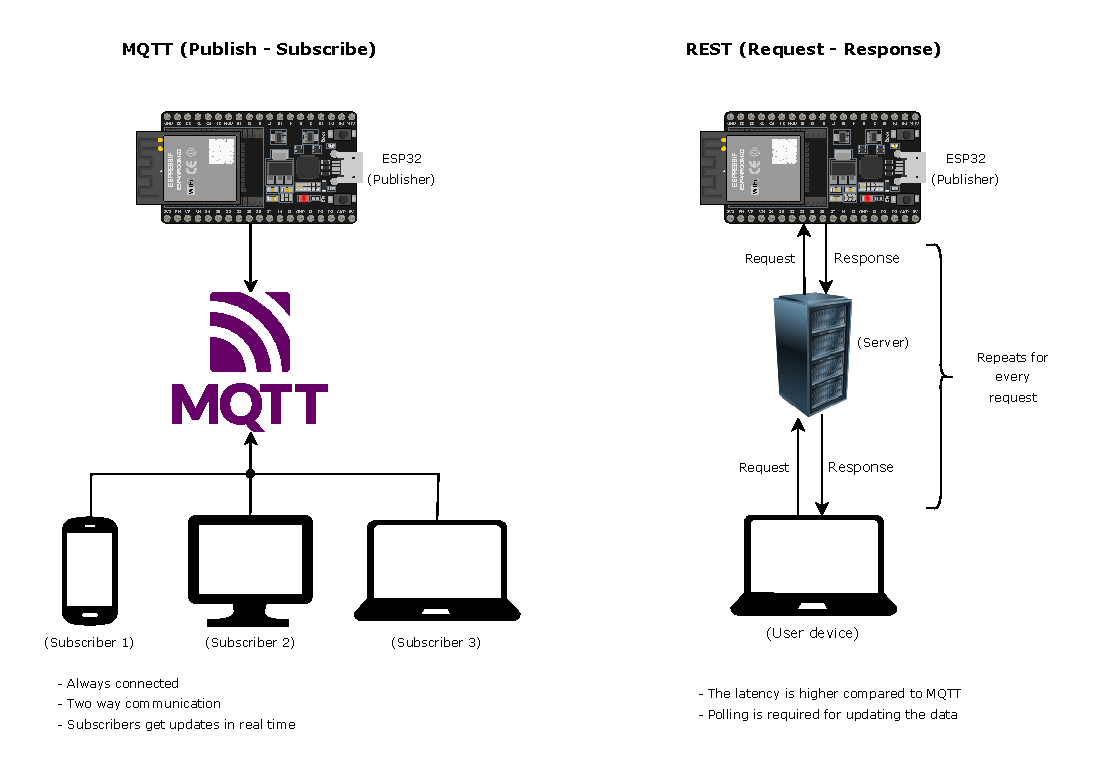
\includegraphics[width=0.9\textwidth]{figuri/MQTT_vs_REST.pdf}
    \caption{Comparație arhitecturală între modelul HTTP cerere-răspuns și modelul \textit{publish/subscribe} bazat pe MQTT}
    \label{fig:mqtt_vs_http}
\end{figure}

În HomeForge folosesc o abordare hibridă, pentru că fiecare protocol are zona în care este eficient:
\begin{itemize}
    \item MQTT pentru comunicația cu dispozitivele fizice — telemetrie și comenzi, în timp real;
    \item HTTP/REST pentru interacțiunea browser--backend — fetch-ul listei de dispozitive, login, profil, layout-ul dashboard-ului.
\end{itemize}
Frontend-ul nu vorbește direct cu brokerul MQTT; el comunică doar cu API-ul REST al Django, iar backend-ul este cel care traduce între cele două lumi.

\begin{table}[htbp]
    \centering
    \caption{MQTT vs. HTTP/REST în context IoT}
    \vspace{0.4\baselineskip}
    \label{tab:mqtt_vs_rest}
    {\setstretch{1.0}
    \footnotesize
    \renewcommand{\arraystretch}{1.15}
    \begin{tabular}{|>{\raggedright\arraybackslash}p{3.2cm}|>{\raggedright\arraybackslash}p{5.8cm}|>{\raggedright\arraybackslash}p{5.8cm}|}
        \hline
        \textbf{Caracteristică} & \textbf{MQTT} & \textbf{HTTP / REST} \\ \hline
        Model & Asincron, \textit{publish-subscribe} (broker) & Sincron, cerere-răspuns \\ \hline
        Overhead antet & de la 2 bytes & sute de bytes (headere, cookies) \\ \hline
        Conexiune TCP & Persistentă (\textit{stateful}) & Per cerere (\textit{stateless}) \\ \hline
        QoS nativ & Da, 3 niveluri & Nu (depinde de aplicație) \\ \hline
        Push server $\rightarrow$ client & Suportat nativ & Necesită \textit{polling} sau WebSocket-uri \\ \hline
        Caz tipic & Telemetrie, microcontrolere & API web, operații CRUD \\ \hline
    \end{tabular}
    }
\end{table}

\section{Platforme open-source: unde se poziționează HomeForge}
Soluțiile open-source dedicate Smart Home-ului sunt deja mature. Cele mai cunoscute, Home Assistant și OpenHAB, au câștigat o tracțiune semnificativă în comunitate prin integrările cu sute de producători, prin suportul pentru protocoale specializate (Zigbee, Z-Wave, KNX, Matter), prin reguli avansate de automatizare construite vizual și prin documentația vastă creată de utilizatori.

Pentru un utilizator final care vrea o casă inteligentă completă, oricare dintre ele este o alegere mai bună decât HomeForge. Diferența este nișa în care lucrăm. HomeForge nu vrea să suporte 100 de producători, nici 10. Vrea să suporte un singur lucru bine: dispozitive făcute manual, pe ESP32, care vorbesc MQTT printr-un format JSON simplu. În schimb, oferă:
\begin{itemize}
    \item un cod sursă scurt (sub 2500 de linii pentru API-ul backend, vezi \texttt{views.py});
    \item zero magie ascunsă — fiecare endpoint este vizibil în \texttt{urls.py};
    \item un \textit{device builder} grafic, care permite construirea unui tip de dispozitiv vizual și exportă firmware-ul ESP32 corespunzător;
    \item o curbă de învățare scăzută pentru studenți, care pot extinde sistemul fără să citească arhitectura unei platforme cu 10 ani de dezvoltare în spate.
\end{itemize}

Cu alte cuvinte, HomeForge nu intră în competiție cu Home Assistant pe terenul lui. Acoperă o zonă diferită: a celui care vrea să prototipeze rapid, să înțeleagă fluxul de date end-to-end și, eventual, să pornească de aici către un sistem mai serios.

\section{Justificarea stivei tehnologice}
Alegerile tehnologice nu sunt accidentale: fiecare componentă rezolvă o problemă concretă pe care am întâlnit-o în implementare. Mai jos justific principalele opțiuni; ele se vor regăsi în capitolele de implementare.

\subsection{Backend: Python, Django și DRF}
Python a fost ales pentru că oferă cele mai mature biblioteci pentru manipularea datelor heterogene (\texttt{paho-mqtt}, \texttt{Pillow}, \texttt{ArduinoJson} la nivel de embed). Django adaugă peste asta un ORM matur, un sistem de migrații versionabil și protecții implicite împotriva atacurilor uzuale (CSRF, XSS, SQL injection). Django REST Framework completează stack-ul cu \textit{serializers}, \textit{viewsets} și \textit{permission classes}, care reduc semnificativ codul boilerplate atunci când construiești un API.

Concret, în HomeForge, un endpoint precum \texttt{POST /api/devices/} este descris în doar câteva zeci de linii, validările sunt declarate în serializer, iar permisiunile sunt asignate per view (vezi \texttt{views.py:376-461}).

\subsection{Bază de date: PostgreSQL cu JSONB}
La nivel de bază de date, am avut nevoie de două lucruri în același loc: relații stricte (un dispozitiv aparține unui utilizator și opțional unei camere) și structuri flexibile (starea curentă a unui dispozitiv este JSON arbitrar). PostgreSQL este unul dintre puținele RDBMS-uri care oferă bine ambele lumi, prin tipul \texttt{JSONB} și suport pentru indexare GIN.

Documentația oficială PostgreSQL precizează că, spre deosebire de tipul \texttt{json} (care păstrează textul JSON brut), \texttt{JSONB} pre-parsează documentul într-un format binar decompus, ceea ce face citirea ulterioară mai rapidă și permite indexare cu \texttt{GIN} pentru căutări în interiorul JSON-ului \cite{postgresql_jsonb_docs}. Pentru o platformă didactică, această combinație este ideală: studenții văd o schemă SQL clară pentru \texttt{User}, \texttt{Room}, \texttt{Device}, dar nu sunt obligați să facă o migrație de fiecare dată când adaugă un senzor cu un format nou.

În cod, decizia se traduce într-un singur câmp:
\begin{minted}{python}
class Device(models.Model):
    # ... relațiile clasice ...
    current_state = models.JSONField(
        default=dict, blank=True,
        help_text="Current state of device controls"
    )
\end{minted}

\subsection{Magistrală de mesaje: MQTT (Mosquitto)}
Pentru implementarea concretă a brokerului, am folosit Mosquitto — open-source, standardizat OASIS, suficient de ușor încât poate rula în același container Docker cu backend-ul. Pe portul implicit 1883, brokerul ascultă atât de la clienții ESP32 cât și de la procesul \texttt{mqtt\_listener} al backend-ului.

În implementarea curentă, mecanismul \textit{Last Will and Testament} oferit de MQTT nu este utilizat; statusul \texttt{offline} este detectat printr-un timer aplicativ, în cadrul comenzii \texttt{mqtt\_listener} — un dispozitiv care nu a publicat în ultimele 30 de secunde este marcat ca \texttt{offline}. Această abordare simplifică firmware-ul ESP32 și centralizează logica de gestionare a stării în partea Python a aplicației.

\subsection{Frontend: React, Next.js și TanStack Query}
Pe partea de UI, dashboard-ul este un \textit{Single Page Application} care își actualizează cardurile în timp real, pe baza datelor preluate de la backend. React rezolvă re-randarea eficientă prin Virtual DOM, iar Next.js oferă deasupra un \texttt{app router} modern, suport \textit{Server-Side Rendering} (pe care nu îl folosesc agresiv în acest proiect) și un sistem de bundling deja optimizat — la combinarea celor două, ecuația practică e că obțin un timp scurt până la prima interacțiune fără să configurez manual Webpack sau alte unelte de build.

În HomeForge folosesc TanStack Query (fost React Query) pentru toată stocarea de date la nivel de client. Decizia este motivată de două lucruri: (1) cache automat și deduplicare a cererilor, (2) suport excelent pentru \textit{optimistic updates}, care este coloana vertebrală a UI-ului responsiv din dashboard. Detaliile sunt în Capitolul 4.

\subsection{Containerizare: Docker și Docker Compose}
Problema „pe calculatorul meu funcționează” este reală în orice proiect cu mai multe servicii. Bellavista și Zanni au demonstrat că este fezabil să rulezi containere Docker chiar și pe noduri Edge cu resurse limitate, cum este Raspberry Pi, ceea ce arată că aceeași imagine se poate distribui fără modificări de la un server la un nod de margine \cite{docker_iot_edge}. În HomeForge:
\begin{itemize}
    \item \texttt{backend} (Django + Mosquitto + Avahi) și \texttt{db} (PostgreSQL) rulează ca două servicii separate;
    \item \texttt{frontend} este al treilea container, cu o imagine Next.js standard;
    \item dezvoltatorul rulează totul cu \texttt{docker compose up}, fără să instaleze nimic local.
\end{itemize}
Pentru dezvoltare rapidă există și varianta \texttt{./dev.sh}, care pornește backend-ul și frontend-ul direct pe mașina gazdă, ocolind containerele.

% FIGURĂ DE ADĂUGAT: o diagramă verticală a stivei tehnologice:
% sus „Frontend (Next.js + React + TanStack Query)”,
% la mijloc „Backend (Django + DRF) + Broker MQTT (Mosquitto) + PostgreSQL”,
% jos „Hardware (ESP32 + senzori DHT11/BMP180 + relee)”.
% Poate fi desenată cu draw.io / Inkscape și exportată ca PDF.
\begin{figure}[htbp]
    \centering
    % 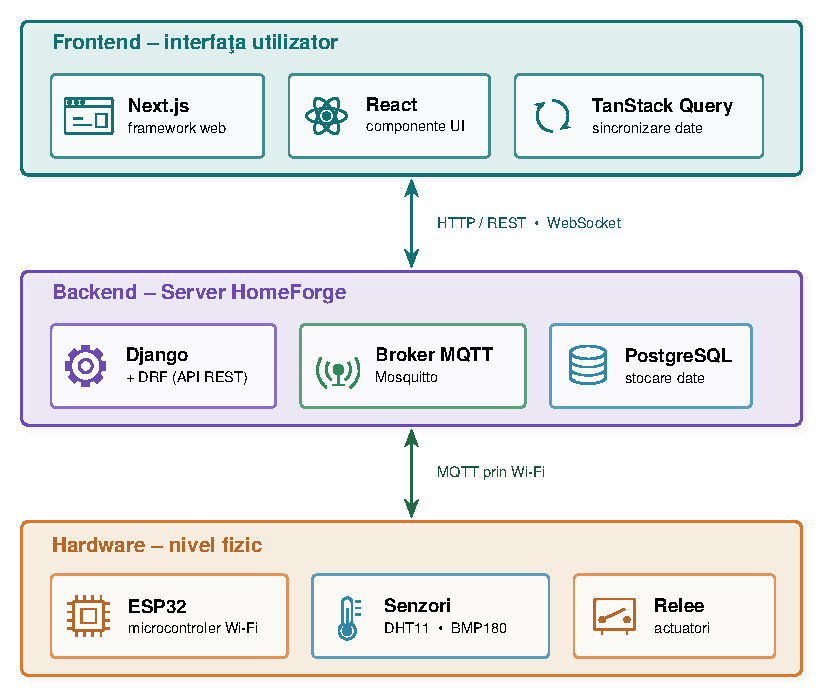
\includegraphics[width=0.7\textwidth]{figuri/stiva_tehnologica.pdf}
    \caption{Stiva tehnologică decuplată a platformei HomeForge (figură de adăugat)}
    \label{fig:tech_stack}
\end{figure}

\chapter{Arhitectura Sistemului HomeForge}

\section{Arhitectura generală și paradigma decuplării}
Pentru a garanta o scalabilitate ridicată și o mentenanță eficientă, platforma HomeForge adoptă o arhitectură orientată pe servicii (\textit{Service-Oriented Architecture}). În mod tradițional, aplicațiile web erau monolitice, serverul fiind responsabil atât de logica de business, cât și de generarea interfeței grafice (HTML). HomeForge abandonează acest model în favoarea unei decuplări totale: logica de prelucrare a datelor (\textit{backend-ul}) acționează ca un punct central de adevăr (\textit{Single Source of Truth}) și expune exclusiv un API (\textit{Application Programming Interface}) de tip RESTful.

\subsection{Justificarea alegerii framework-ului backend}
Pentru implementarea backend-ului, s-a optat pentru limbajul Python 3.12+ și framework-ul Django, acompaniat de \textit{Django REST Framework} (DRF). Această alegere tehnologică a fost motivată de două aspecte fundamentale: maturitatea ecosistemului Python în manipularea datelor (esențială pentru parsarea telemetriei IoT) și securitatea robustă oferită \textit{out-of-the-box} de Django împotriva vulnerabilităților web comune (SQL Injection, XSS).

Importanța utilizării standardului REST în acest context este subliniată de Pautasso et al.: \textit{„Serviciile web RESTful oferă un set de constrângeri arhitecturale care garantează scalabilitatea, performanța independentă și portabilitatea, elemente vitale pentru ecosistemele IoT unde nodurile hardware au putere de calcul limitată”} \cite{rest_api_architecture}. Prin această decuplare, API-ul dezvoltat poate servi nu doar interfața web actuală (Next.js), ci și viitoare aplicații mobile sau scripturi de automatizare, fără a necesita modificări ale codului de bază.

\section{Modelarea datelor: Puterea PostgreSQL și JSONB}
Sistemul de gestiune a bazelor de date (SGBD) ales este PostgreSQL 15. Într-un mediu IoT, provocarea principală a stocării datelor este eterogenitatea senzorilor. Bazele de date relaționale clasice sunt rigide, în timp ce bazele de date NoSQL (precum MongoDB) sacrifică integritatea relațională (\textit{referential integrity}) pentru flexibilitate.

PostgreSQL a fost ales deoarece oferă „cel mai bun din ambele lumi” prin intermediul tipului de date \texttt{JSONB}. Conform cercetărilor conduse de Izquierdo et al., \textit{„Tipul de date JSONB din PostgreSQL oferă performanțe de interogare și indexare comparabile cu bazele de date NoSQL dedicate, menținând în același timp garanțiile tranzacționale ACID necesare unui sistem de producție”} \cite{jsonb_postgresql}.

\subsection{Abordarea \textit{Schema-less} pentru starea dispozitivelor}
HomeForge folosește o structură hibridă de date. Entitatea principală păstrează relațiile stricte (către cameră, tip de dispozitiv, utilizator), dar starea hardware-ului este stocată într-un câmp flexibil denumit \texttt{current\_state}. Pentru a demonstra această flexibilitate, prezentăm modul în care sistemul stochează stările pentru dispozitive complet diferite în aceeași coloană, evitând necesitatea unor noi migrații SQL la adăugarea unui senzor DIY nou:

\begin{minted}{json}
// 1. Modul releu simplu (Bec inteligent)
{"relay_1": true, "brightness": 75}

// 2. Termostat inteligent (Senzor + Actuator)
{"target_temp": 22.5, "current_temp": 21.3, "mode": "heat"}

// 3. Placă de dezvoltare DIY cu 4 relee
{"relay_1": false, "relay_2": true, "relay_3": true, "relay_4": false}
\end{minted}

La nivel de backend, această schemă este definită clar prin ORM-ul (\textit{Object-Relational Mapping}) din Django:

\begin{minted}{python}
from django.db import models

class Device(models.Model):
    name = models.CharField(max_length=100)
    ip_address = models.GenericIPAddressField()
    status = models.CharField(max_length=20, default='offline')
    # Relații FK către entitățile organizatorice (Relațional pur)
    room = models.ForeignKey('Room', on_delete=models.SET_NULL, null=True)
    device_type = models.ForeignKey('CustomDeviceType', on_delete=models.PROTECT)
    # Stocarea dinamică a stării (NoSQL hibrid)
    current_state = models.JSONField(default=dict)
\end{minted}

\section{Securitate, Optimizare și Structura API-ului}

\subsection{Securitate și Controlul Accesului (JWT \& RBAC)}
Metoda tradițională de autentificare web, bazată pe sesiuni și \textit{cookies}, este ineficientă pentru aplicațiile decuplate și vulnerabilă la atacuri de tip CSRF (\textit{Cross-Site Request Forgery}). Prin urmare, HomeForge a implementat standardul \textit{JSON Web Tokens} (JWT).

Referitor la securitatea arhitecturilor IoT moderne, Ali et al. notează: \textit{„Autentificarea bazată pe token-uri JSON elimină necesitatea stocării stării sesiunii pe server (stateless authentication), reducând semnificativ consumul de memorie centrală și oferind o metodă securizată și ușoară de verificare a identității la nivelul nodurilor din rețea”} \cite{jwt_security_iot}.

Sistemul integrează un mecanism ierarhic de tip RBAC (\textit{Role-Based Access Control}): primul utilizator înregistrat devine \texttt{owner} (cu privilegii de administrare a infrastructurii hardware și software), următorii putând fi asociați rolurilor de \texttt{admin}, \texttt{user} sau \texttt{viewer} (acces \textit{read-only} la rețea).

\subsection{Optimizarea interogărilor SQL (Problema N+1)}
În dezvoltarea cu ORM-uri, o greșeală comună care degradează masiv latența este "Problema N+1". Fără optimizări, pentru a afișa 50 de dispozitive pe ecranul principal, backend-ul ar efectua o interogare pentru lista dispozitivelor și încă 50 de interogări distincte pentru a afla camera fiecăruia. 

Platforma rezolvă matematic această ineficiență prin dictarea explicită a preluării anticipate a datelor, generând sub capotă interogări SQL complexe de tip \texttt{INNER JOIN}:

\begin{minted}{python}
# Optimizare a interogărilor pentru modelul Device
Device.objects.select_related(
    'room', 'user', 'device_type', 'device_type__card_template'
).prefetch_related(
    'device_type__card_template__controls'
)
\end{minted}
Prin această arhitectură, timpul de procesare rămâne constant O(1) la nivel de accesare a bazei de date, indiferent de dimensiunea rețelei fizice.

\section{Arhitectura și Specificațiile Interfeței de Programare (API)}

Pentru expunerea completă a capabilităților sistemului, API-ul platformei HomeForge a fost proiectat conform standardelor RESTful, operând ca strat intermediar între baza de date PostgreSQL, nodurile IoT și interfața utilizatorului. Această secțiune detaliază contractele de date (\textit{endpoints}), permisiunile asociate și logica de business implementată.

\subsection{Sistemul de Control al Accesului (RBAC)}
Întregul API este securizat prin intermediul \textit{JSON Web Tokens} (JWT), necesitând prezența antetului \texttt{Authorization: Bearer <token>} pentru rutele protejate. Spre deosebire de sistemele simple cu un singur nivel de administrare, platforma utilizează o ierarhie complexă bazată pe roluri (RBAC):
\begin{itemize}
    \item \textbf{Owner (Proprietar):} Cel mai înalt nivel de privilegii. Primul utilizator care apelează ruta de înregistrare primește automat acest rol, având control absolut.
    \item \textbf{Admin:} Poate gestiona utilizatorii, camerele, echipamentele și aprobările pentru noile tipuri de hardware.
    \item \textbf{User (Standard):} Poate controla starea dispozitivelor proprii și poate propune (fără a aproba) arhitecturi noi de hardware.
    \item \textbf{Viewer:} Are acces strict de citire (\textit{read-only}) asupra panoului de control.
\end{itemize}

\subsection{Autentificare și Gestiunea Utilizatorilor}
Acest modul expune funcționalitățile de creare a conturilor, emitere a token-urilor și administrare a profilurilor.

\begin{description}
    \item[\textbf{POST} \texttt{/register/} și \textbf{POST} \texttt{/login/}] \hfill \\
    \textit{Acces: Public.} Rutele procesează credențialele (impunând o politică de parole de minimum 4 caractere și o majusculă) și returnează perechea de token-uri \texttt{access} (valabilitate scurtă, 5 minute) și \texttt{refresh} (valabilitate lungă, 1 zi).
    \item[\textbf{POST} \texttt{/token/refresh/}] \hfill \\
    \textit{Acces: Public.} Permite reînnoirea token-ului de acces fără re-autentificare, vital pentru menținerea unei sesiuni fluide în aplicația de tip \textit{Single Page Application} (SPA).
    \item[\textbf{GET / PUT} \texttt{/me/}] \hfill \\
    \textit{Acces: Orice utilizator autentificat.} Permite utilizatorului curent să își gestioneze preferințele, inclusiv încărcarea unei imagini de profil (\textit{avatar}) de tip \textit{multipart/form-data} și definirea unei culori de accent (\texttt{accent\_color}) pentru personalizarea interfeței.
    \item[\textbf{GET / PUT} \texttt{/users/\{id\}/}] \hfill \\
    \textit{Acces: Admin sau Owner.} Oferă administratorilor posibilitatea de a vizualiza toți utilizatorii din ecosistem și de a suprascrie (\textit{override}) datele sau rolul oricărui cont.
\end{description}

\subsection{Topologia Fizică: Camere și Dispozitive}
Aceste endpoint-uri gestionează partiționarea fizică și înregistrarea senzorilor în rețeaua locală.

\begin{description}
    \item[\textbf{GET/POST/PUT/DELETE} \texttt{/rooms/}] \hfill \\
    \textit{Acces modificare: Admin/Owner.} Permite organizarea hardware-ului pe camere. Sistemul implementează un mecanism de siguranță: la apelarea metodei \texttt{DELETE} pe o cameră, dispozitivele asociate nu sunt șterse, ci câmpul lor devine \texttt{room = null}, fiind transferate în starea „Neasignat”.
    \item[\textbf{GET/POST} \texttt{/devices/}] \hfill \\
    \textit{Acces: Orice utilizator autentificat.} Permite înregistrarea unui nou nod IoT. Validarea backend-ului asigură că adresa \texttt{ip\_address} este un IPv4 valid și că \texttt{device\_type}-ul asociat a fost aprobat anterior de un administrator.
\end{description}

\subsection{Mecanismul principal de gestiune a stării (\textit{State Control})}
Modulul de control reprezintă componenta critică a arhitecturii IoT, fiind optimizat pentru a masca latența inerentă rețelelor hardware.

\begin{description}
    \item[\textbf{PATCH} \texttt{/devices/\{id\}/state/}] \hfill \\
    \textit{Acces: Orice utilizator autentificat.} Recepționează comenzi parțiale (ex. doar \texttt{\{"brightness": 75\}}). Backend-ul aplică logica de îmbinare (\textit{merge}) cu starea curentă din baza de date și returnează un cod \texttt{HTTP 202 Accepted}, semnalând interfeței să se actualizeze instantaneu (\textit{Optimistic UI}), în timp ce comanda reală este transmisă asincron prin MQTT. De asemenea, API-ul efectuează maparea dinamică automată: o comandă trimisă către un identificator generic precum \texttt{relay\_1} este rutată corect către widget-ul hardware specific (ex. \texttt{switch-177}).
\end{description}

\subsection{Platforma de Crowdsourcing: Fluxul Tipului de Dispozitive}
Pentru a evita fenomenul de \textit{vendor lock-in}, HomeForge permite comunității să propună definiții pentru echipamente DIY (ex. plăci cu ESP32), implementând un flux de aprobare riguros.

\begin{description}
    \item[\textbf{POST} \texttt{/device-types/propose/}] \hfill \\
    \textit{Acces: Orice utilizator autentificat.} Receptează o structură JSON complexă care include atât arhitectura nodurilor (microcontroler, senzori, pini PWM), cât și tiparul vizual pentru UI (\texttt{card\_template}). Starea inițială este setată forțat la \texttt{approved: false}.
    \item[\textbf{GET} \texttt{/admin/device-types/pending/} și \textbf{GET} \texttt{.../denied/}] \hfill \\
    \textit{Acces: Admin/Owner.} Listează separat definițiile care așteaptă revizuirea și cele care au fost respinse.
    \item[\textbf{PUT / PATCH} \texttt{/admin/device-types/\{id\}/}] \hfill \\
    \textit{Acces: Admin/Owner.} Permite administratorului să corecteze erorile dintr-o propunere (ex. o mapare greșită a unui widget) înainte de a o aproba.
    \item[\textbf{POST} \texttt{.../approve/} și \textbf{POST} \texttt{.../deny/}] \hfill \\
    \textit{Acces: Admin/Owner.} Tranzitează starea propunerii. La respingere, API-ul solicită obligatoriu un motiv (\texttt{rejection\_reason}) pentru a oferi feedback utilizatorului inițiator. Tipurile respinse pot fi ulterior curățate în bloc (\textit{Bulk Delete}) via ruta \texttt{/admin/device-types/denied/delete/}.
\end{description}

\subsection{Sistemul Multi-Nivel de Notificări}
Infrastructura de alertare a fost dezvoltată pentru a monitoriza proactiv starea rețelei și a utilizatorilor, generând 10 tipuri distincte de evenimente (de la informații de sistem la deconectări critice de hardware).

\begin{description}
    \item[\textbf{GET} \texttt{/notifications/} și \textbf{GET} \texttt{/notifications/unread-count/}] \hfill \\
    \textit{Acces: Orice utilizator autentificat.} Returnează alerte filtrate pe niveluri de prioritate (\texttt{low, normal, high, urgent}). Ruta de contorizare (\texttt{unread-count}) a fost special optimizată pentru a fi interogată periodic (\textit{polling}) la fiecare 30 de secunde de către interfața web.
    \item[\textbf{POST} \texttt{/notifications/read-all/} și \textbf{DELETE} \texttt{/notifications/bulk-delete/}] \hfill \\
    \textit{Acces: Orice utilizator autentificat.} Permit operațiuni în bloc asupra alertelor.
    \item[\textbf{POST} \texttt{/admin/notifications/broadcast/}] \hfill \\
    \textit{Acces: Admin/Owner.} Permite difuzarea unui mesaj global, având ca țintă toți utilizatorii (\texttt{all}), doar administratorii (\texttt{admins}) sau doar vizitatorii (\texttt{viewers}).
\end{description}

\subsection{Persistența Interfeței și Randarea Topologiei}
HomeForge nu depinde de stocarea locală a browserului (\textit{localStorage}), ci implementează un motor propriu de sincronizare a preferințelor vizuale pe server.

\begin{description}
    \item[\textbf{GET} \texttt{/topology/}] \hfill \\
    \textit{Acces: Orice utilizator autentificat.} Procesează datele din PostgreSQL și le formatează direct în standardul cerut de librăria React Flow (matrice de Noduri și Muchii), calculând poziția radială, statusul de conectare și culorile specifice (\texttt{\#10B981} pentru online, \texttt{\#EF4444} pentru offline).
    \item[\textbf{PUT} \texttt{/dashboard-layout/}] \hfill \\
    \textit{Acces: Orice utilizator autentificat.} Salvează configurația personalizată de grilă (\textit{Grid}) a utilizatorului. JSON-ul stochează ordinea cardurilor și permite gruparea dispozitivelor în dosare (\textit{Folders}) de 2-4 elemente, simulând comportamentul aplicațiilor mobile native. Endpoint-ul folosește o semantică de tip \textit{upsert} și validează strict integritatea ID-urilor transmise.

\begin{minted}{json}
{
  "version": 1,
  "items": [
    { "type": "device", "deviceId": 5 },
    {
      "type": "folder",
      "folderId": "folder-m1kx2j-a3b7",
      "name": "Living Room",
      "deviceIds": [1, 3]
    }
  ]
}
\end{minted}

    \item[\textbf{GET} \texttt{/dashboard-layout/} (Lanțul de Fallback)] \hfill \\
    La interogare, sistemul aplică un lanț inteligent de rezoluție: încearcă returnarea \textit{Layout-ului Personal} $\rightarrow$ dacă nu există, returnează \textit{Layout-ul Partajat (Shared)} setat de Admin $\rightarrow$ dacă nu există, returnează \texttt{null}.
    \item[\textbf{PATCH} \texttt{/device-order/}] \hfill \\
    \textit{Acces: Orice utilizator autentificat.} Permite actualizarea exclusivă a preferinței de sortare a echipamentelor pe ecran (\texttt{room}, \texttt{type}, \texttt{status}, \texttt{name} sau \texttt{custom}), fără a necesita re-salvarea întregii structuri JSON a panoului de control.
\end{description}

\section{Mecanisme Avansate: UX și Persistență}

\subsection{Mascarea latenței prin Actualizări Optimiste (\textit{Optimistic UI})}
În IoT-ul bazat pe Edge Computing, dispozitivele fizice (microcontrolerele) pot fi în modul \textit{Deep Sleep} sau pot suferi întârzieri de rețea. Dacă serverul ar bloca firul de execuție până la comutarea fizică a unui releu, experiența utilizatorului ar fi considerată lentă și defectuoasă. 

Acest fenomen este contracarat conceptual prin arhitectura \textit{Optimistic UI}. Literatura de specialitate referitoare la interacțiunea om-calculator sugerează că: \textit{„Mascarea latenței rețelei prin prezentarea imediată a stării vizuale anticipate, înainte de validarea finală a serverului, crește masiv nivelul de fluiditate perceput și reduce frustrarea utilizatorului în sistemele distribuite”} \cite{latency_ux_optimistic}.

Implementarea tehnică constă în procesarea asincronă: o cerere \texttt{PATCH} către \texttt{/devices/\{id\}/state/} nu așteaptă senzorul. Backend-ul îmbină datele, validează structura logică și răspunde imediat cu starea previzionată (\texttt{HTTP 202 Accepted}), în timp ce confirmarea MQTT operează independent în fundal:

\begin{minted}{json}
{
  "status": "Command sent",
  "detail": "State will update when device confirms.",
  "device_status": "online",
  "current_state": {
    "relay_1": true,
    "brightness": 75
  }
}
\end{minted}

\subsection{Motorul de Sincronizare a Interfeței (\textit{Dashboard Layout Sync})}
Spre deosebire de aplicațiile simple care salvează aranjamentul elementelor grafice pe memoria locală a browser-ului (\textit{localStorage}), HomeForge folosește un sistem de \textit{upsert} pe server. Această alegere asigură coerența interfeței (utilizatorul găsește butoanele exact în aceeași ordine atât pe laptop, cât și pe mobil).

Configurația interfeței, reprezentată mai jos, stochează nu doar ordinea absolută, ci și grupările logice (\textit{Folders}):

\begin{minted}{json}
{
  "version": 1,
  "items": [
    { "type": "device", "deviceId": 5 },
    {
      "type": "folder",
      "folderId": "folder-abc-123",
      "name": "Living Room",
      "deviceIds": [1, 3]
    }
  ]
}
\end{minted}

Motorul de backend nu execută doar o stocare oarbă a acestui JSON, ci rulează un \textit{Sanity Check}: validează unicitatea fiecărui \texttt{deviceId} și aplică un lanț de rezervă (\textit{fallback chain}). Dacă un cont nou nu posedă o configurație proprie, backend-ul îi servește automat varianta \textit{Shared Layout}, definită în prealabil de administratorul sistemului.
\chapter{Aplicația web Next.js}

\section{Structura proiectului}
Aplicația de frontend este construită cu Next.js 16 și React 19 (vezi \texttt{package.json}). Folosește \textit{App Router}-ul Next.js, ceea ce înseamnă că rutele sunt definite implicit prin structura folderelor din directorul \texttt{app/}. Două rute sunt publice și separate de zona autentificată:
\begin{itemize}
    \item \texttt{app/login/} — formular de autentificare;
    \item \texttt{app/register/} — formular de înregistrare;
    \item \texttt{app/setup/} — \textit{setup wizard}-ul afișat când backend-ul răspunde cu \texttt{is\_fresh: true}.
\end{itemize}

Restul aplicației trăiește sub \texttt{/dashboard/...} și folosește un layout comun definit în \texttt{layout.tsx}. Acesta verifică, la fiecare reîncărcare, profilul curent prin \texttt{fetchProfile()} și redirecționează către \texttt{/login} dacă răspunsul este \texttt{401}. Tot el inserează \texttt{SidebarProvider}-ul, breadcrumb-urile dinamice și butonul de schimbare a temei (light/dark).

Sub \texttt{/dashboard} găsim:
\begin{itemize}
    \item \texttt{page.tsx} — dashboard-ul principal cu cardurile dispozitivelor;
    \item \texttt{devices/} — lista detaliată a dispozitivelor;
    \item \texttt{device-builder/} — editorul vizual pentru tipuri de dispozitive (\textit{device builder});
    \item \texttt{device-collection/} — vitrina de tipuri propuse de comunitate;
    \item \texttt{device-types/} — pagina cu tipurile de dispozitive disponibile;
    \item \texttt{topology/} — vizualizarea de topologie cu React Flow;
    \item \texttt{settings/} — pagina de setări utilizator;
    \item \texttt{admin/} — secțiune restricționată cu sub-paginile \texttt{approvals/}, \texttt{users/}, \texttt{rooms/}, \texttt{device-types/}, \texttt{debug/}.
\end{itemize}

Componentele reutilizabile sunt în \texttt{components/}, grupate pe domenii: \texttt{devices/} pentru cardurile de dispozitive, \texttt{device-builder/} pentru editorul vizual, \texttt{notifications/} pentru centrul de notificări, \texttt{setup/} pentru wizardul inițial, \texttt{topology/} pentru nodurile React Flow și \texttt{ui/} pentru primitive (Button, Card, Slider, etc.) generate prin \texttt{shadcn/ui}.

% FIGURĂ DE ADĂUGAT: arborele de directoare al folderului frontend/app
% și frontend/components — poate fi un text formatat sau un export
% din IDE/Treerunner.
\begin{figure}[htbp]
    \centering
    % \includegraphics[width=0.7\textwidth]{figuri/frontend_tree.pdf}
    \caption{Structura directoarelor aplicației Next.js (figură de adăugat)}
    \label{fig:frontend_tree}
\end{figure}

\section{Stack-ul de interfață: shadcn/ui, Radix și Tailwind}
Înainte de a intra în paginile concrete, este utilă o privire asupra straturilor de UI care le compun. HomeForge nu folosește o singură bibliotecă de componente „închisă" (în stilul Material UI sau Ant Design), ci o stivă compusă din trei nivele, fiecare cu un rol bine definit.

\paragraph{Tailwind CSS 4 — sistemul de stiluri.} Tailwind este folosit drept singura unealtă de stilizare; nu există fișiere CSS scrise de mână (cu excepția lui \texttt{globals.css}, care declară doar variabilele de temă și câteva animații \texttt{@keyframes}). Tot ce înseamnă spațiere, tipografie, culori, breakpoints este exprimat prin clase utilitare direct în JSX. Decizia, pe lângă viteza de iterare, are un avantaj practic: un component poate fi mutat sau copiat fără să trebuiască să sincronizez și un fișier CSS separat.

\paragraph{Radix UI — primitivele de comportament.} Pentru toate elementele care au logică interactivă complexă (Dropdown, Dialog, Popover, Slider, Switch, Select, Tooltip, Tabs, Collapsible, Avatar, Scroll Area), HomeForge folosește primitivele \texttt{@radix-ui/react-*}. Acestea oferă comportamentul corect din punct de vedere accesibilitate (focus trap, navigare cu tastatura, atribute \texttt{aria-*}, gestiunea \texttt{Escape}), dar fără niciun stil impus — partea vizuală o pune Tailwind.

\paragraph{shadcn/ui — stratul de „componente proprii".} Deasupra Radix-ului trăiește un al treilea nivel pe care îl materializează \texttt{shadcn/ui}. Acesta nu este o bibliotecă instalată ca dependință \texttt{npm}, ci un CLI care \emph{copiază} cod TypeScript direct în repository-ul meu, în \texttt{components/ui/}. Configurația proiectului (\texttt{components.json}) declară stilul „new-york", \texttt{rsc=true}, \texttt{tsx=true}, \texttt{baseColor=neutral}, \texttt{iconLibrary=lucide} și aliasurile de import \texttt{@/components}, \texttt{@/lib/utils}, \texttt{@/components/ui}, \texttt{@/hooks}.

Diferența față de o bibliotecă tradițională este filozofică, dar contează: codul fiecărui Button, Card, Dialog \emph{îmi aparține} și pot să-l modific fără să mă confrunt cu API-ul cuiva. Folderul \texttt{components/ui/} conține 28 de astfel de componente — printre ele \texttt{button.tsx}, \texttt{card.tsx}, \texttt{dialog.tsx}, \texttt{dropdown-menu.tsx}, \texttt{slider.tsx}, \texttt{sidebar.tsx}, \texttt{tabs.tsx}, \texttt{tooltip.tsx}, \texttt{command.tsx}, \texttt{markdown-editor.tsx} — toate generate inițial cu shadcn/ui, apoi adaptate la nevoile mele.

Pentru a vedea pe ce se sprijină acest model, exemplific cu \texttt{Button}, unde apar și \texttt{class-variance-authority} (cva) și utility-ul \texttt{cn} compus din \texttt{clsx} + \texttt{tailwind-merge}:

\begin{minted}{tsx}
const buttonVariants = cva("inline-flex items-center ...", {
  variants: {
    variant: { default: "...", destructive: "...", outline: "...",
               secondary: "...", ghost: "...", link: "..." },
    size:    { default: "h-9 px-4 py-2", sm: "h-8 px-3",
               lg: "h-10 px-6", icon: "size-9", ... },
  },
  defaultVariants: { variant: "default", size: "default" },
})
\end{minted}
\texttt{cva} permite definirea variantelor ca o tabelă declarativă, iar \texttt{cn} din \texttt{lib/utils.ts} rezolvă coliziunile între clase Tailwind:
\begin{minted}{typescript}
import { clsx, type ClassValue } from "clsx"
import { twMerge } from "tailwind-merge"
export function cn(...inputs: ClassValue[]) {
  return twMerge(clsx(inputs))
}
\end{minted}
Combinația elimină categoria de bug-uri în care două clase Tailwind conflictuale (\texttt{p-2} și \texttt{p-4}, de exemplu) ar fi aplicate amândouă într-o ordine nedeterministă.

\paragraph{Lucide React — iconițe.} Toate iconițele din aplicație vin din pachetul \texttt{lucide-react}, ales prin \texttt{components.json} (\texttt{"iconLibrary": "lucide"}). În \texttt{lib/icons.ts}, expun tot setul ca un map, ceea ce permite construirea componentei \texttt{IconPicker} (vezi \texttt{components/devices/IconPicker.tsx}) — un \texttt{Popover} cu căutare în interiorul căruia utilizatorul poate alege orice icon Lucide pentru o cameră sau un dispozitiv:
\begin{minted}{typescript}
import * as LucideIcons from 'lucide-react';
export const ICON_MAP = LucideIcons as unknown as Record<string, any>;
export const ICON_OPTIONS = Object.keys(ICON_MAP).filter(key => {
  return /^[A-Z]/.test(key) && key !== 'Icon' && typeof ICON_MAP[key] !== 'undefined';
});
\end{minted}

\paragraph{Sonner — sistemul de toast.} Pentru notificările inline (succes, eroare, info), folosesc biblioteca \texttt{sonner}, accesată prin singleton-ul \texttt{toast} din \texttt{components/ui/sonner.tsx}. Apelurile sunt scurte și consistente:
\begin{minted}{typescript}
toast.success("Layout set as default for all users");
toast.error("Failed to sync device state", { description: err.message });
\end{minted}

\paragraph{Framer Motion — animații.} Animațiile (carduri care intră cu fade-in, folderul care se deschide cu \texttt{AnimatePresence}, etc.) sunt gestionate de \texttt{framer-motion}. În cardurile cu drag-and-drop folosesc \texttt{@dnd-kit/core}, \texttt{@dnd-kit/sortable} și \texttt{@dnd-kit/utilities} — toate trei făcând parte din aceeași familie de pachete.

\paragraph{Restul pieselor.} Pe lângă cele de mai sus, mai există câteva dependențe utilitare pe care le menționez în trecere: \texttt{date-fns} pentru manipulare de date și ore, \texttt{cmdk} pentru paleta de comandă, \texttt{prismjs} cu \texttt{react-simple-code-editor} pentru editor-ul de cod din device builder, \texttt{react-markdown} împreună cu \texttt{remark-gfm} și \texttt{rehype-highlight} pentru randarea documentației Markdown, iar \texttt{elkjs} este disponibilă pentru viitoarele layout-uri automate ale grafurilor (este în \texttt{dependencies}, dar nu o folosesc activ încă).

% FIGURĂ DE ADĂUGAT: screenshot al unei pagini din UI cu accent vizual pe
% câteva primitive de la shadcn/ui — un Dialog deschis, un Dropdown, un
% Toast Sonner activ în colț. Util pentru a arăta consistența vizuală.
\begin{figure}[htbp]
    \centering
    % \includegraphics[width=0.95\textwidth]{figuri/ui_components_overview.png}
    \caption{Captură de ecran: primitive shadcn/ui în acțiune (Dialog, Dropdown, Toast) — screenshot de adăugat}
    \label{fig:ui_primitives}
\end{figure}

\section{Layout-ul aplicației: sidebar, breadcrumbs, header}
Întreaga zonă autentificată folosește un layout comun \texttt{app/dashboard/layout.tsx}, care montează patru piese fixe: \texttt{AppSidebar}, butonul de \texttt{SidebarTrigger}, breadcrumb-urile dinamice și \texttt{ModeToggle}-ul pentru tema light/dark.

\subsection{Sidebar-ul adaptiv}
\texttt{components/app-sidebar.tsx} construiește meniul lateral pornind de la rolul utilizatorului curent. Lista de bază este aceeași pentru toți (Dashboard, Device Builder, Device Collection, Topology, Settings), iar dacă rolul este \texttt{admin} sau \texttt{owner}, se adaugă un submeniu „Admin Panel" cu link-uri către \emph{Rooms}, \emph{Users}, \emph{Device Types} și \emph{Debug}:
\begin{minted}{typescript}
const navMain = React.useMemo(() => {
  const items = [
    { title: "Dashboard", url: "/dashboard", icon: LayoutDashboard, isActive: true },
    { title: "Device Builder", url: "/dashboard/device-builder", icon: Cpu },
    { title: "Device Collection", url: "/dashboard/device-collection", icon: Package },
    { title: "Topology", url: "/dashboard/topology", icon: Network },
    { title: "Settings", url: "/dashboard/settings", icon: Settings },
  ];
  if (isAdmin) {
    items.push({
      title: "Admin Panel", url: "/dashboard/admin", icon: Shield,
      items: [
        { title: "Rooms", url: "/dashboard/admin/rooms", icon: Home },
        { title: "Users", url: "/dashboard/admin/users", icon: Users },
        { title: "Device Types", url: "/dashboard/admin/device-types", icon: Cpu },
        { title: "Debug", url: "/dashboard/admin/debug", icon: Bug },
      ]
    });
  }
  return items;
}, [isAdmin]);
\end{minted}

Componenta de bază (\texttt{Sidebar}, \texttt{SidebarHeader}, \texttt{SidebarFooter}, \texttt{SidebarContent}) vine din shadcn/ui și expune un \texttt{SidebarProvider} care gestionează starea „colapsat / expandat" — fiind responsivă, pe mobil se transformă într-un \texttt{Sheet} care alunecă din lateral, iar pe desktop poate fi colapsată la doar iconițe. Header-ul conține logo-ul HomeForge (componenta \texttt{HomeForgeLogo}, un SVG inline), iar footer-ul găzduiește un \texttt{NavUser} cu avatarul utilizatorului, numele și un dropdown de „Sign out".

% FIGURĂ DE ADĂUGAT: screenshot al sidebar-ului expandat pe stânga,
% cu utilizator în rol Owner — se văd toate cele 5 voci principale plus
% sub-meniul „Admin Panel". Sugestie: face screenshot la 1920x1080,
% taie zona din stânga (sidebar + ~30% din pagină).
\begin{figure}[htbp]
    \centering
    % 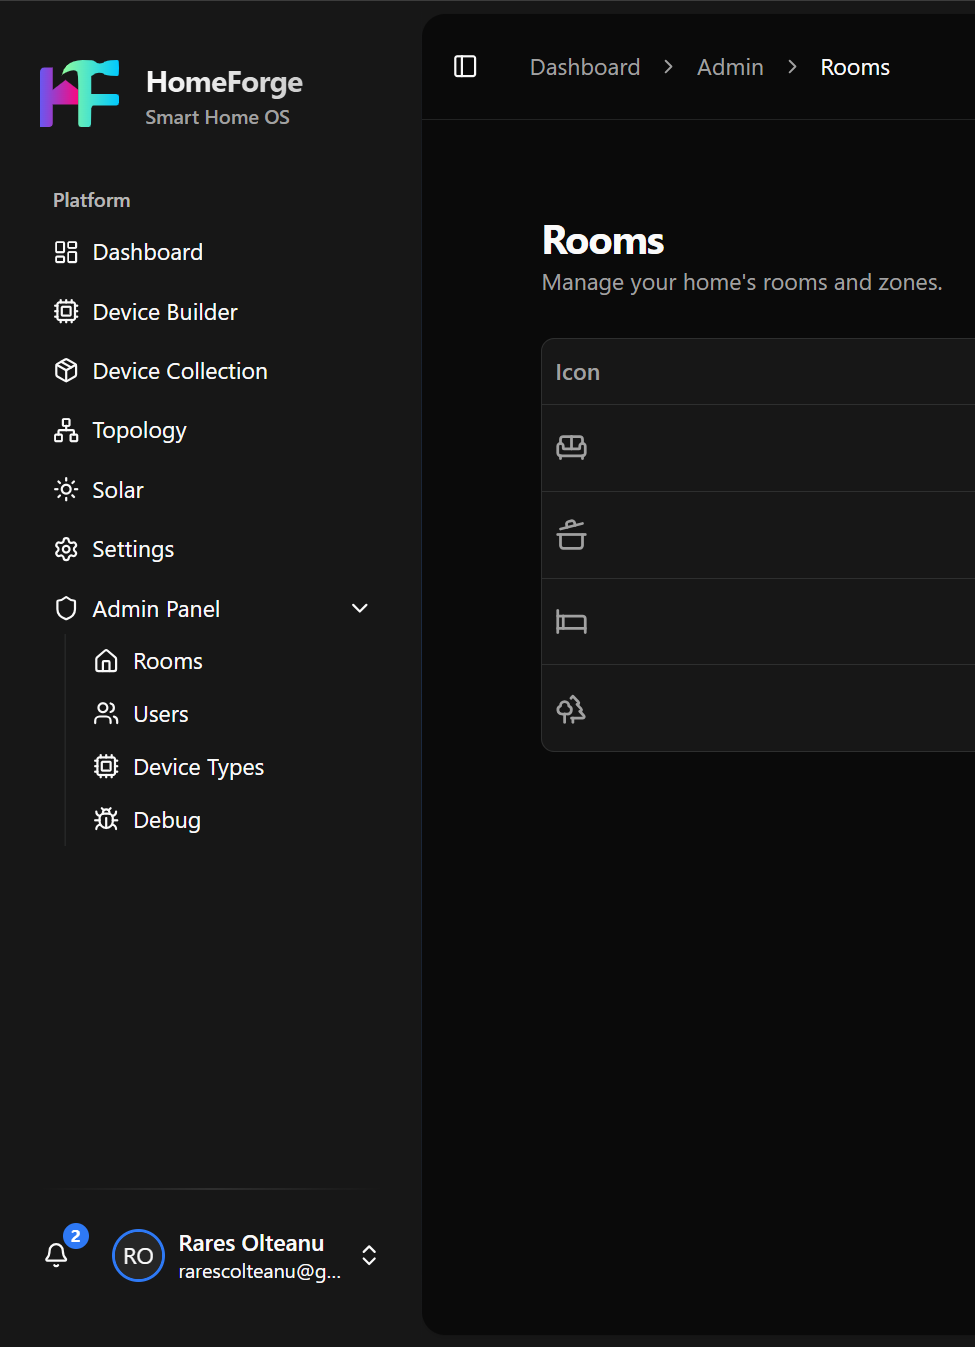
\includegraphics[width=0.5\textwidth]{figuri/sidebar_admin.png}
    \caption{Sidebar-ul HomeForge cu sub-meniul \emph{Admin Panel} activ (screenshot de adăugat)}
    \label{fig:sidebar_admin}
\end{figure}

\subsection{Breadcrumb-uri dinamice}
Componenta \texttt{DynamicBreadcrumbs} citește path-ul curent prin \texttt{usePathname()} din \texttt{next/navigation} și îl segmentează automat. Asta înseamnă că la \texttt{/dashboard/admin/device-types?filter=pending} apar trei breadcrumb-uri (\emph{Dashboard $>$ Admin $>$ Device Types}) fără ca eu să fi configurat ceva explicit. Capitalizarea, hyphen-to-space și link-urile către nivelurile părinte se calculează în timpul randării.

\subsection{Tema și culorile de accent}
Tema light/dark este oferită de pachetul \texttt{next-themes}, care setează un atribut \texttt{class} pe \texttt{<html>}. Butonul \texttt{ModeToggle} din header comută între cele două.

Pe lângă temă, fiecare utilizator își poate alege o \emph{culoare de accent}. Valorile disponibile sunt declarate în \texttt{components/user-provider.tsx}:
\begin{minted}{typescript}
export const ACCENT_COLORS = {
  default: "oklch(0.205 0 0)",
  violet:  "oklch(0.5 0.2 280)",
  blue:    "oklch(0.5 0.2 250)",
  green:   "oklch(0.6 0.15 150)",
  orange:  "oklch(0.6 0.15 50)",
  pink:    "oklch(0.6 0.2 340)",
  cyan:    "oklch(0.6 0.15 200)",
}
\end{minted}
Sunt definite în spațiul de culoare OKLCH (preferabil fa\c{t}\u{a} de RGB pentru consistență perceptivă), iar funcția \texttt{applyAccentColor} setează direct variabilele CSS \texttt{--primary} și \texttt{--ring} pe \texttt{document.documentElement}, fără reload. Preferința este persistată pe server (câmpul \texttt{accent\_color} din \texttt{Profile} — vezi Capitolul 3) și replicată în \texttt{localStorage} pentru a evita „flash"-ul vizual la prima încărcare; un \texttt{useLayoutEffect} aplică culoarea înainte de paint.

% FIGURĂ DE ADĂUGAT: două screenshot-uri ale aceleiași pagini Settings,
% unul cu accent violet și unul cu accent cyan, alăturate, pentru a arăta
% cum se schimbă instantaneu tema.
\begin{figure}[htbp]
    \centering
    % \includegraphics[width=0.95\textwidth]{figuri/accent_colors.png}
    \caption{Aceea\c{s}i pagină \emph{Settings} cu două accent colors diferite (screenshot de adăugat)}
    \label{fig:accent_colors}
\end{figure}

\subsection{\texttt{UserProvider} — sursa unică de adevăr pe client}
\texttt{components/user-provider.tsx} expune un Context React care:
\begin{itemize}
    \item încarcă profilul curent la mount (\texttt{loadUser}) — întâi din \texttt{localStorage} pentru a evita „flash of unauthenticated content", apoi se actualizează cu răspunsul real al lui \texttt{fetchProfile()};
    \item aplică culoarea de accent;
    \item gestionează logout-ul: golește cache-ul TanStack Query (\texttt{queryClient.clear()}), șterge token-urile, șterge layout-ul cache-uit local și redirecționează la \texttt{/login}.
\end{itemize}
Importanța pașilor de cleanup la logout nu este teoretică: fără \texttt{queryClient.clear()}, dacă un alt utilizator se loghează imediat după pe același browser, ar vedea pentru câteva secunde dispozitivele utilizatorului precedent.

\section{Stratul de comunicare cu API-ul}
Toate apelurile către backend sunt concentrate în fișierul \texttt{apiClient.js}, scris în JavaScript pur. Alegerea de a nu folosi TypeScript pentru acest modul a fost deliberată: păstrează codul la nivelul unui apel \texttt{fetch} standard și facilitează parcurgerea sa de către cititori familiarizați cu API-ul \texttt{fetch} al browserelor.

\subsection{Determinarea URL-ului backend-ului}
Frontend-ul nu cunoaște la build-time IP-ul gazdei pe care va rula. Funcția \texttt{getBackendUrl} folosește locația curentă a browserului și înlocuiește portul cu 8000:
\begin{minted}{javascript}
export function getBackendUrl() {
  if (typeof window !== 'undefined') {
    return `${window.location.protocol}//${window.location.hostname}:8000`;
  }
  return 'http://localhost:8000';
}
\end{minted}
Practic, dacă un utilizator accesează aplicația de pe \texttt{http://192.168.1.10:3000}, cererile vor merge automat către \texttt{http://192.168.1.10:8000}, fără configurări suplimentare.

\subsection{Gestiunea token-urilor JWT}
La login, token-ul de acces și cel de refresh sunt stocate în \texttt{localStorage}. Toate cererile autentificate trec prin \texttt{fetchWithAuth}, care:
\begin{enumerate}
    \item adaugă antetul \texttt{Authorization: Bearer <token>};
    \item dacă răspunsul este \texttt{401}, apelează \texttt{refreshAccessToken()} și reîncearcă cererea o singură dată;
    \item dacă reîmprospătarea eșuează, șterge token-urile și aruncă o eroare cu \texttt{status = 401}, care este capturată de \texttt{dashboard/layout.tsx} și care redirecționează către \texttt{/login}.
\end{enumerate}
\begin{minted}{javascript}
async function fetchWithAuth(url, options = {}) {
  const headers = { ...options.headers, ...getAuthHeaders() };
  let res = await fetch(url, { ...options, headers });
  if (res.status === 401) {
    const newToken = await refreshAccessToken();
    const newHeaders = { ...options.headers, Authorization: `Bearer ${newToken}` };
    res = await fetch(url, { ...options, headers: newHeaders });
  }
  return res;
}
\end{minted}

\subsection{Tratarea uniformă a erorilor}
Funcția \texttt{handleApiError} parsează formatul standard al erorilor returnate de Django REST Framework. Aceasta gestionează trei cazuri: un câmp \texttt{detail} (de obicei la erori de permisiune), un câmp \texttt{non\_field\_errors} (la validări la nivel de serializer) și restul, în care fiecare cheie este un câmp specific cu o listă de mesaje. Mesajele sunt concatenate și aruncate ca un singur \texttt{Error}, pe care UI-ul îl afișează prin \texttt{toast.error}.

\section{Gestiunea stării: TanStack Query}
HomeForge folosește \textit{TanStack Query} (denumit anterior React Query) pentru toate datele la nivel de aplicație. \texttt{QueryProvider} este montat în root-ul aplicației (\texttt{components/query-provider.tsx}) și expune un singur \texttt{QueryClient}. Fiecare componentă apoi consumă două hook-uri: \texttt{useQuery} pentru fetch-uri (lista de dispozitive, profilul, notificările) și \texttt{useMutation} pentru scrieri (toggle, update, delete). Două decizii de configurare merită evidențiate: lista de dispozitive folosește \texttt{refetchInterval: 3000} (polling la 3 secunde, înlocuind o eventuală conexiune WebSocket), iar contorul de notificări necitite folosește \texttt{refetchInterval: 30000} (30 de secunde, suficient pentru un badge fără a încărca inutil backend-ul).

\section{Dashboard-ul principal}
Pagina \texttt{app/dashboard/page.tsx} orchestrează trei surse de date — dispozitive, tipuri de dispozitive și camere — și le combină într-un singur grid. Există cinci moduri de grupare expuse într-un \texttt{<Select>}:
\begin{itemize}
    \item \texttt{all} — toate dispozitivele, în ordinea aleasă de utilizator (mod cu drag-and-drop);
    \item \texttt{room} — grupare pe cameră;
    \item \texttt{type} — grupare pe tipul de dispozitiv;
    \item \texttt{status} — grupare pe \texttt{Online} / \texttt{Offline} / \texttt{Error};
    \item \texttt{name} — sortare alfabetică simplă.
\end{itemize}
La nivel de cod, modul curent (\texttt{viewMode}) este oglindit într-o variabilă \texttt{deviceOrder} pe care \texttt{useDashboardLayout} o sincronizează cu serverul prin endpoint-ul \texttt{PATCH /api/device-order/}. Preferința utilizatorului supraviețuiește între dispozitive.

\subsection{Hook-ul \texttt{useDashboardLayout}}
Logica de layout este izolată într-un singur hook (\texttt{hooks/useDashboardLayout.ts}). Acesta:
\begin{enumerate}
    \item descarcă layout-ul curent prin \texttt{useQuery(['dashboardLayout'], fetchDashboardLayout)} cu \texttt{staleTime: Infinity};
    \item dacă API-ul eșuează (mod offline), cade pe \texttt{localStorage} ca rezervă;
    \item \textit{reconciliază} layout-ul cu lista actuală de dispozitive — elimină referințele către cele șterse, adaugă cele noi, dizolvă folderele rămase cu mai puțin de 2 elemente (vezi \texttt{reconcileLayout} în \texttt{lib/dashboard-grid.ts});
    \item expune funcții de mutație: \texttt{moveItem}, \texttt{createFolder}, \texttt{addToFolder}, \texttt{removeFromFolder}, \texttt{renameFolder}, \texttt{dissolveFolder}, \texttt{resetLayout}, \texttt{revertToShared};
    \item salvează modificările pe server cu \texttt{debounce} de 800 ms și \textit{flush} imediat la ieșirea din modul de editare („Done”).
\end{enumerate}

\begin{minted}{typescript}
const scheduleSave = useCallback((newLayout: DashboardLayout) => {
  saveLayout(newLayout);                         // localStorage instantaneu
  if (saveTimerRef.current) clearTimeout(saveTimerRef.current);
  hasPendingSaveRef.current = true;
  saveTimerRef.current = setTimeout(() => {
    saveToApi(newLayout);                        // API după 800 ms
  }, 800);
}, [saveToApi]);
\end{minted}

\subsection{Drag-and-drop și foldere}
Componenta \texttt{DraggableDeviceGrid} folosește biblioteca \texttt{@dnd-kit/core} pentru drag-and-drop. Fiecare card este învelit într-un \texttt{SortableGridItem} cu trei zone de drop:
\begin{itemize}
    \item zona \emph{stângă}: dispozitivul tras este inserat înaintea țintei;
    \item zona \emph{dreaptă}: este inserat după;
    \item zona \emph{mijloc}: dispozitivele se combină într-un folder nou (sau dispozitivul este adăugat în folderul țintă).
\end{itemize}
Constrângerile semantice (un folder are între 2 și 4 dispozitive, fiecare \texttt{deviceId} apare cel mult o dată) sunt verificate atât pe client cât și pe backend (vezi \texttt{DashboardLayoutSerializer} în Capitolul 3).

% FIGURĂ DE ADĂUGAT: screenshot al dashboard-ului în mod „edit” — se văd cardurile,
% un folder deschis cu 3 dispozitive, plus indicatorii de drop (stânga / mijloc / dreapta).
\begin{figure}[htbp]
    \centering
    % \includegraphics[width=0.95\textwidth]{figuri/dashboard_edit_mode.png}
    \caption{Dashboard-ul HomeForge în modul de editare a layout-ului (screenshot de adăugat)}
    \label{fig:dashboard_edit}
\end{figure}

\section{Cardurile inteligente: \texttt{SmartDeviceCard}}
Componenta \texttt{SmartDeviceCard} este probabil cea mai densă din întregul frontend, fiindcă rezolvă în același loc trei probleme dificile: randarea dinamică a unui număr variabil de widget-uri, optimistic UI și combaterea \textit{glitch}-urilor de stare la apăsări rapide.

\subsection{Randarea condusă de \texttt{card\_template}}
Fiecare tip de dispozitiv definește o listă de \texttt{controls}, în care fiecare element are un \texttt{widget\_type}. Componenta apelează funcția internă \texttt{renderWidget(control, index)}, care selectează implementarea vizuală corespunzătoare: \texttt{Switch} pentru \texttt{TOGGLE}, \texttt{Slider} pentru \texttt{SLIDER} sau widget-uri specializate definite în \texttt{SensorWidgets.tsx} (\texttt{TemperatureWidget}, \texttt{HumidityWidget} etc.). Fiecare widget primește valoarea curentă prin câmpul \texttt{variable\_mapping}, mecanism care permite aceleiași componente să servească orice tip de dispozitiv definit prin device builder.

Layout-ul cardului are două variante: \emph{row} (widget-uri pe linie, util pentru dispozitive simple) și \emph{square} (widget-uri pătrate, util pentru senzori). Layout-ul de grid se citește dintr-un câmp \texttt{layout\_config} cu chei \texttt{w} (numărul de coloane) și \texttt{gap}; componenta convertește \texttt{layout\_config.w} sau \texttt{layout\_config.columns} în clase Tailwind (\texttt{grid-cols-1/2/3}).

Există și un caz special: \texttt{isSingleToggleDevice(controls)}. Dacă un dispozitiv are exact un singur control de tip \texttt{TOGGLE} și nimic altceva (un releu pentru un bec, de exemplu), cardul devine \emph{tap-to-toggle} — întreaga suprafață a cardului acționează ca un switch, fără un widget separat. Detaliul îmbunătățește vizibil ergonomia pe mobil.

\subsection{Pattern-ul \textit{Optimistic UI}}
Această subsecțiune descrie mecanismul central de gestiune a stării interactive. La apăsarea unui toggle, componenta:
\begin{enumerate}
    \item construiește noua stare locală \texttt{newState = \{...currentState, [variable]: value\}};
    \item o salvează imediat în \texttt{useState}, deci UI-ul se actualizează în 0 milisecunde;
    \item programează un \texttt{setTimeout} de 50 ms (pentru toggle, ca să consolideze apăsările repetate) sau 500 ms (pentru slider, ca să nu trimită zeci de cereri per gest) — un \textit{debounce} clasic;
    \item după timer, declanșează mutația TanStack Query, care apelează \texttt{updateDeviceState(id, newState)}.
\end{enumerate}

Mutația utilizează patru dintre hook-urile expuse de \texttt{useMutation} — \texttt{mutationFn}, \texttt{onMutate}, \texttt{onError} și \texttt{onSettled}. Hook-ul \texttt{onSuccess} este omis deliberat, din motive explicate mai jos. Scheletul implementării, în formă condensată:
\begin{minted}{typescript}
const updateMutation = useMutation({
  mutationFn: ({ id, newState }) => updateDeviceState(id, newState),
  onMutate: async ({ id, newState }) => {
    await queryClient.cancelQueries({ queryKey: ['devices'] });
    const previousDevice = queryClient.getQueryData(['device', id]);
    queryClient.setQueryData(['device', id], (old) => ({ ...old, current_state: newState }));
    return { previousDevice };                       // pasat la onError pentru rollback
  },
  onError:   (_e, _v, ctx) => { /* rollback la ctx.previousDevice + toast.error */ },
  onSettled: () => { /* setIsRefetching(true); invalidate cu delay; timeout siguranță 5s */ },
});
\end{minted}

Câteva detalii subtile pe care le-am implementat după mai multe iterații:
\begin{itemize}
    \item \texttt{onMutate} salvează starea anterioară într-un \textit{context} care, în caz de eroare, este folosit pentru \emph{rollback}. Fără aceasta, dacă dispozitivul este offline, butonul ar rămâne blocat în starea optimistă incorectă.
    \item Intenționat \emph{nu} folosesc \texttt{onSuccess} pentru a suprascrie starea locală: serverul răspunde imediat cu \texttt{HTTP 202} și o stare anticipată, dar starea reală vine asincron, de pe MQTT. Dacă aș suprascrie pe \texttt{onSuccess}, butonul ar putea „sări” înapoi câteva secunde mai târziu.
    \item \texttt{onSettled} marchează \texttt{isRefetching = true}, ceea ce face ca UI-ul să afișeze un \texttt{Loader2} suprapus. Există un timeout de siguranță (5 secunde) care anulează această stare dacă backend-ul nu mai răspunde — nu vrem ca utilizatorul să rămână blocat cu un \textit{spinner} infinit.
    \item Există un \texttt{useEffect} care detectează când starea de pe server „a ajuns din urmă” starea optimistă (toate cheile modificate sunt egale) și, în acel moment, oprește \texttt{isRefetching}, iar vizual butonul rămâne în stare „sincronizare” doar atât timp cât chiar este o discrepanță reală între ce vrem și ce raportează firmware-ul.
\end{itemize}

% FIGURĂ DE ADĂUGAT: diagrama temporală a unei apăsări — buton apăsat la t=0,
% UI optimist la t=0+ε, debounce până la t=50ms, request HTTP, răspuns 202 la t=100ms,
% publicare MQTT, ESP32 toggle releu la t=180ms, publish state, listener Django,
% refresh listă dispozitive la t=300ms, sincronizat la t=350ms. Poate fi
% o diagramă de tip swim-lane în draw.io.
\begin{figure}[htbp]
    \centering
    % 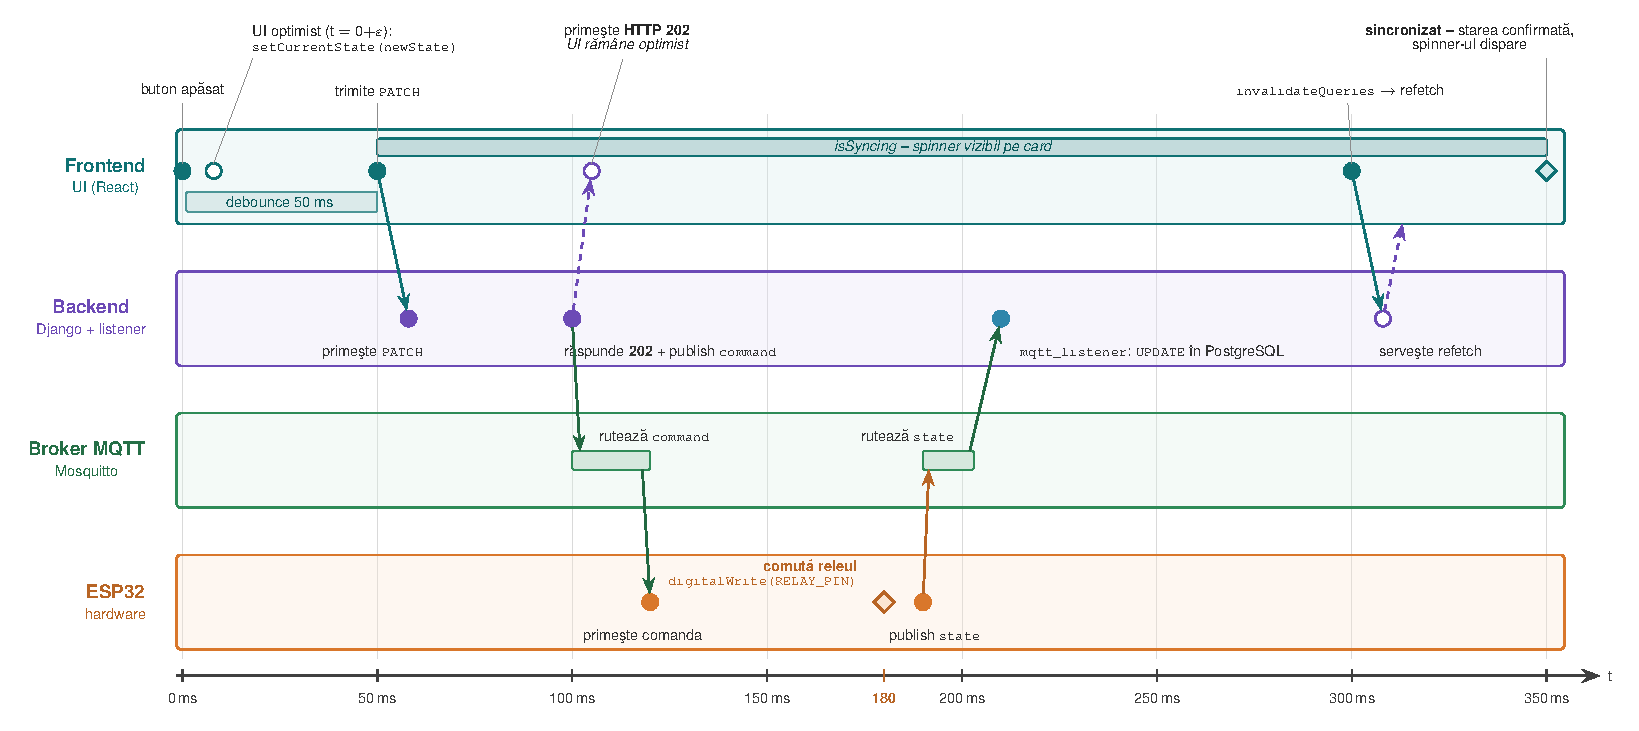
\includegraphics[width=0.95\textwidth]{figuri/optimistic_ui_timeline.pdf}
    \caption{Diagrama temporală a unei apăsări de toggle în interfața HomeForge (figură de adăugat)}
    \label{fig:optimistic_timeline}
\end{figure}

\section{Centrul de notificări}
\texttt{notification-center.tsx} este componenta din colțul dreapta-sus al headerului. Este un \texttt{Popover} care afișează lista alertelor curente:
\begin{itemize}
    \item folosește două \texttt{useQuery} — unul pentru lista completă, unul pentru contorul de necitite, ambele cu \texttt{refetchInterval: 30000};
    \item iconițele și culorile sunt alese în funcție de \texttt{notification\_type} (\texttt{device\_offline}, \texttt{device\_type\_pending}, etc.);
    \item \texttt{action\_url}-ul venit de la backend este normalizat printr-o funcție \texttt{getActionUrl} care adaugă prefixul \texttt{/dashboard} și redirecționează URL-urile către individuale (\texttt{/admin/device-types/22}) către pagina-listă cu filtru (\texttt{/dashboard/admin/device-types?filter=pending}).
\end{itemize}

\section{Vizualizarea topologiei}
Pagina \texttt{/dashboard/topology/} se bazează pe biblioteca \texttt{@xyflow/react} (React Flow v12). Datele vin direct de la endpoint-ul \texttt{GET /api/topology/}, în formatul cerut nativ de React Flow (\texttt{nodes[]} și \texttt{edges[]}). Logica frontend este în \texttt{TopologyCanvas.tsx} și are două componente:

\begin{enumerate}
    \item Un algoritm propriu de layout ierarhic care plasează gateway-ul în stânga și dispozitivele într-o coloană verticală în dreapta, cu \texttt{childXOffset = 450} și \texttt{childSpacingY = 180} pixeli. Renunțarea la un algoritm generic precum ELK sau Dagre este motivată de profilul tipic al rețelei vizualizate: pentru un număr de dispozitive cuprins între 5 și 30, o dispunere în coloană oferă cea mai bună lizibilitate.
    \item Un mecanism de păstrare a selecției: utilizatorul poate selecta unul sau mai multe noduri, iar la re-randarea automată (lista de dispozitive se actualizează la fiecare 3 secunde), un \texttt{useRef} numit \texttt{selectionRef} reține ce a fost selectat și restaurează starea pe noile noduri.
\end{enumerate}

Nodurile sunt randate de patru componente custom în \texttt{topology/nodes/}: \texttt{BuilderStyleNode}, \texttt{GlassDeviceNode}, \texttt{TopologyBuilderNode}, \texttt{UnifiDeviceNode}. \texttt{TopologyBuilderNode} este cea folosită în mod implicit; celelalte sunt variante stilistice între care utilizatorul poate alege.

\section{Editorul vizual de tipuri de dispozitive (\textit{device builder})}
Una dintre cele mai interesante pagini este \texttt{device-builder/DeviceUICreator.tsx}, un editor vizual cu două panouri:
\begin{itemize}
    \item în stânga, un \emph{node graph} (bazat tot pe React Flow) unde utilizatorul adaugă microcontrolere și senzori, conectându-i între ei. Fiecare nod are un ID unic care va fi referențiat din widget-urile vizuale;
    \item în dreapta, lista \emph{widget-urilor} (toggle, slider, sensor) care vor compune cardul dispozitivului. Fiecare widget este legat de un nod prin câmpul \texttt{variable\_mapping}.
\end{itemize}

În jurul editorului există trei panouri auxiliare:
\begin{itemize}
    \item \texttt{FirmwareCodeEditor.tsx} — editor de cod Arduino bazat pe \texttt{prismjs} și \texttt{react-simple-code-editor};
    \item \texttt{WiringDiagramEditor.tsx} — încărcare de schemă electrică (imagine) și descriere textuală;
    \item \texttt{DocumentationEditor.tsx} — editor Markdown cu randare \texttt{react-markdown} (cu \texttt{remark-gfm} și \texttt{rehype-highlight}).
\end{itemize}

La finalul fluxului, utilizatorul apasă \emph{Propose} și aplicația apelează \texttt{POST /api/device-types/propose/} cu o structură JSON compusă din:
\begin{itemize}
    \item \texttt{name} — denumirea tipului;
    \item \texttt{definition.structure[]} — noduri și conexiuni (microcontroler, senzori, pini, fire);
    \item \texttt{card\_template.controls[]} — widget-urile vizuale;
    \item \texttt{firmware\_code}, \texttt{wiring\_diagram\_text}, \texttt{documentation} — text;
    \item \texttt{wiring\_diagram\_base64}, \texttt{documentation\_images\_base64} — imagini encodate.
\end{itemize}
Validatorul de backend (\texttt{CustomDeviceTypeSerializer.validate}) verifică explicit că fiecare \texttt{variable\_mapping} din widget-uri corespunde unui ID definit în \texttt{structure[]} — astfel, este imposibil să propui un tip de dispozitiv „rupt”.

% FIGURĂ DE ADĂUGAT: screenshot al device builder-ului — în stânga node-graph
% cu un ESP32 conectat la DHT11 și un releu, în dreapta lista de widget-uri (un
% TOGGLE pentru releu, un TEMPERATURE pentru DHT11, un HUMIDITY pentru DHT11).
\begin{figure}[htbp]
    \centering
    % 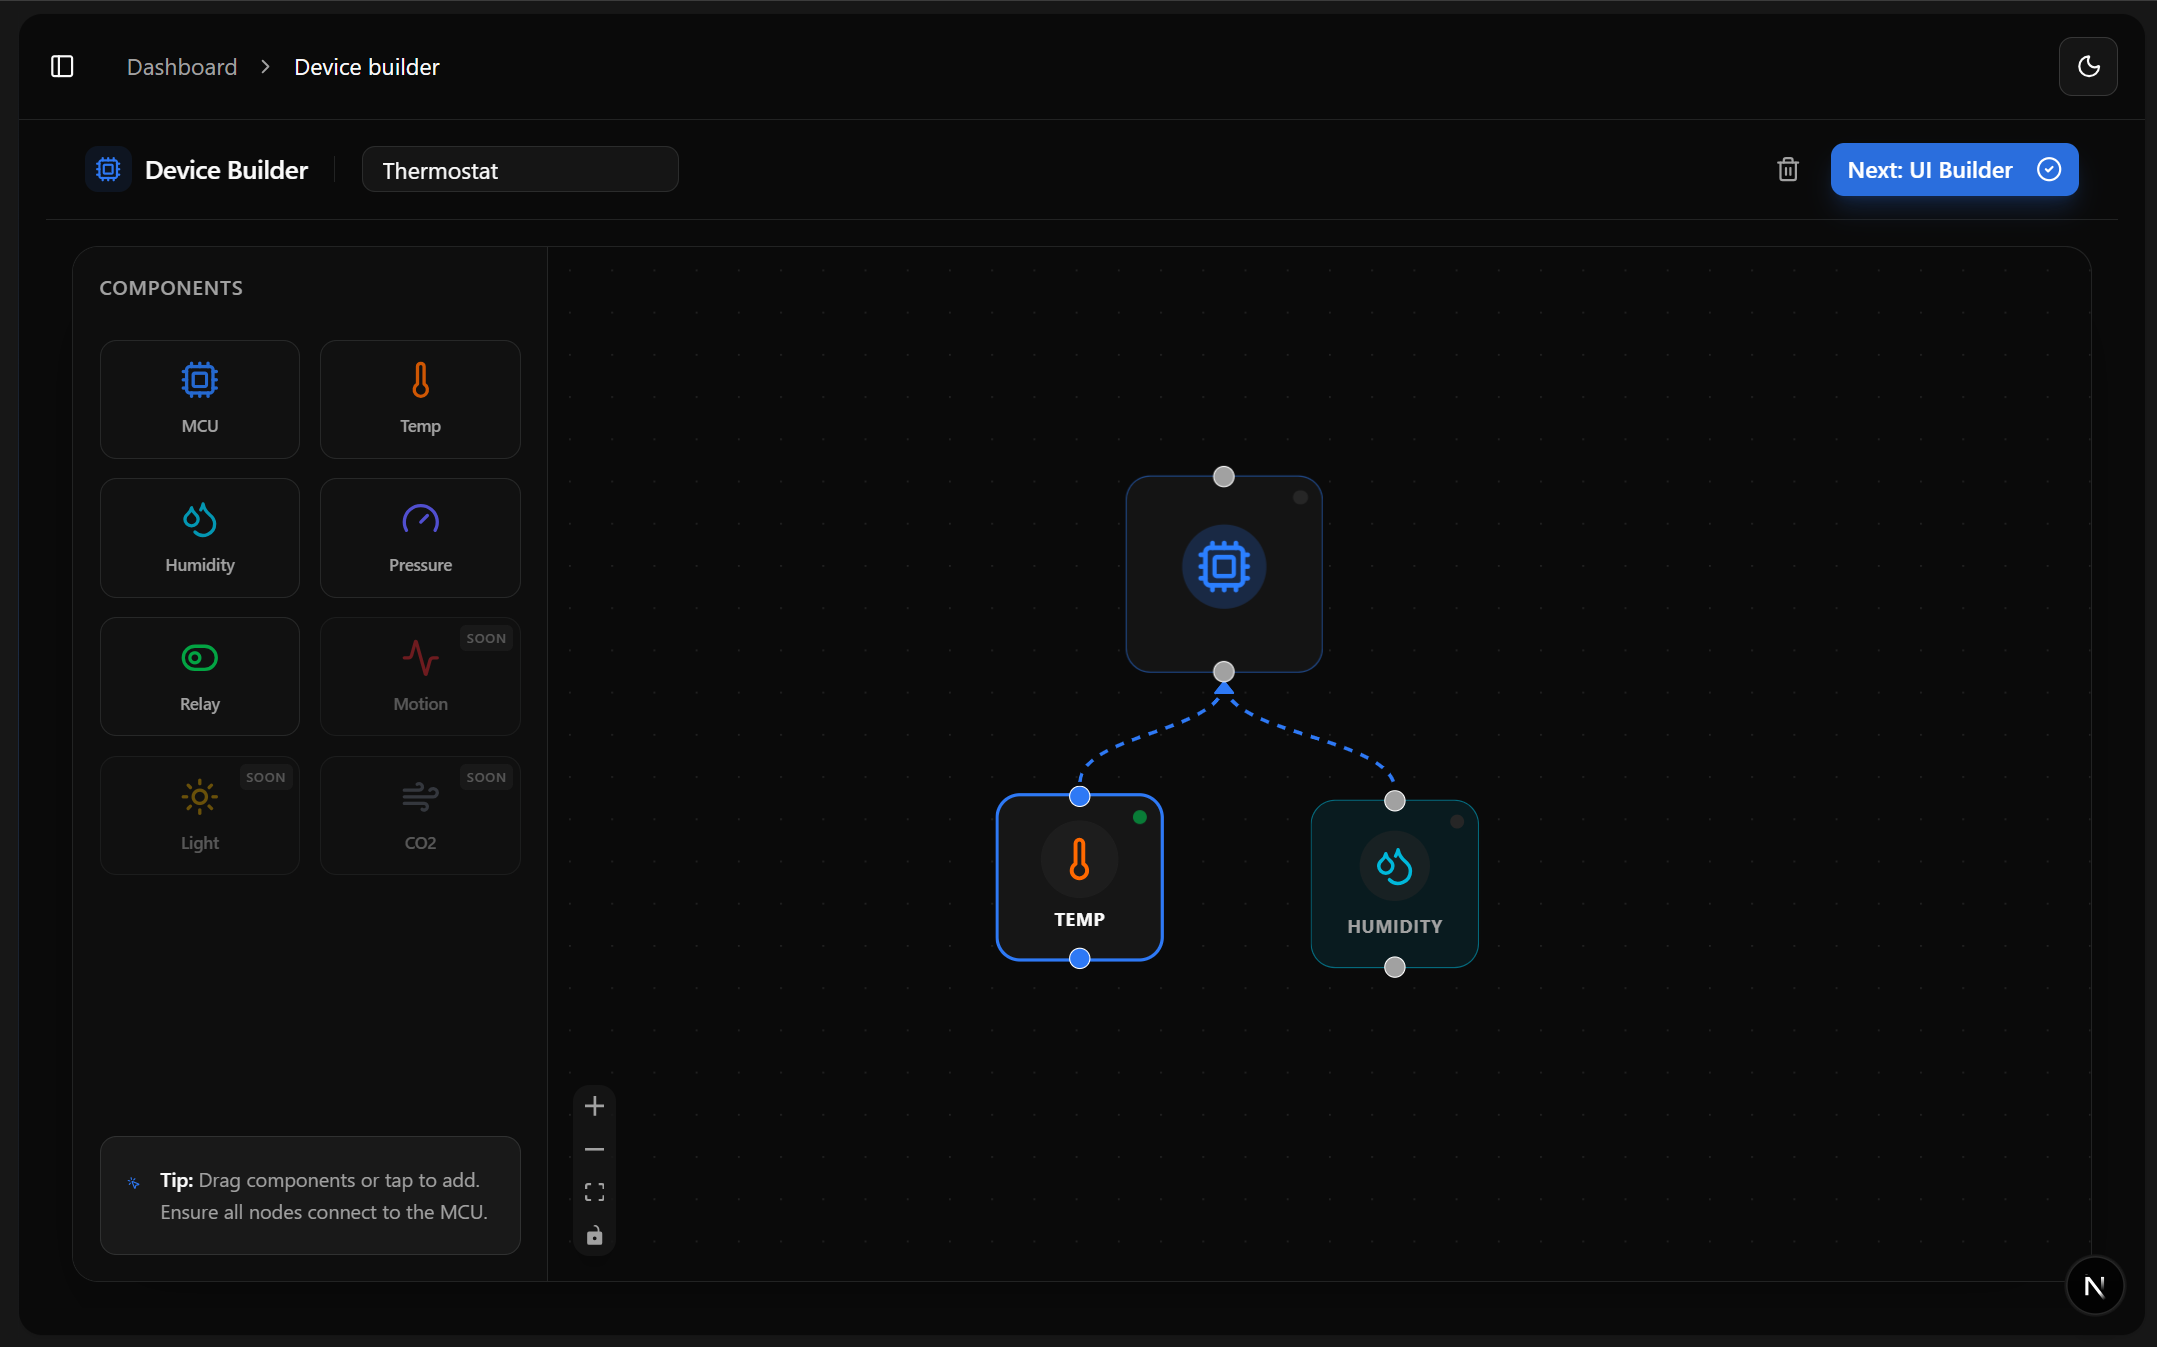
\includegraphics[width=0.95\textwidth]{figuri/device_builder.png}
    \caption{Device builder-ul HomeForge cu un node graph și panoul de widget-uri (screenshot de adăugat)}
    \label{fig:device_builder}
\end{figure}

\section{Setup wizard-ul}
La primul vizit pe o instanță proaspătă, \texttt{SetupWizard.tsx} ghidează utilizatorul printr-un flux în 5 pași: \emph{welcome} → \emph{account} → \emph{rooms} → \emph{devices} → \emph{complete}. Pașii sunt componente separate în \texttt{components/setup/steps/} și comunică prin \texttt{onNext} / \texttt{onBack} cu containerul. La pasul \emph{account}, contul creat devine automat \texttt{owner}, fiindcă serverul răspunde la \texttt{POST /register/} cu \texttt{is\_first\_user} activat (vezi Capitolul 3). La pasul \emph{devices}, utilizatorul poate importa tipurile predefinite prin endpoint-ul \texttt{POST /api/device-types/import-defaults/}.

Indicatorul de progres este o linie întreruptă în patru segmente; fiecare segment primește clase Tailwind diferite pe baza indexului pasului curent. Animațiile de tranziție folosesc \texttt{animate-in fade-in duration-300} — o clasă utilitară oferită de pluginul \texttt{tw-animate-css}.

\section{Onboarding-ul: \texttt{OnboardingChecklist} și \texttt{PageTooltip}}
Asistentul de configurare inițial (\emph{setup wizard}) acoperă doar primii pași de instalare. Pentru utilizatorii care accesează aplicația ulterior, este oferit un mecanism de onboarding suplimentar, mai puțin intruziv, format din două componente complementare situate în \texttt{components/onboarding/}.

\paragraph{Checklist-ul de pe dashboard.} Componenta \texttt{OnboardingChecklist.tsx} este un card afișat în partea superioară a dashboard-ului, vizibil până la finalizarea tuturor pașilor recomandați: crearea contului, definirea a cel puțin unei camere, importul a cel puțin unui tip de dispozitiv și adăugarea primului dispozitiv. Verificarea condițiilor utilizează contoarele primite prin \texttt{props}, cu fallback către apelurile \texttt{fetchRooms()}, \texttt{fetchDeviceTypes()} și \texttt{fetchDevices()}; pașii satisfăcuți sunt marcați automat ca \emph{completați}. Pașii suplimentari sunt persistați în \texttt{localStorage} sub cheia \texttt{onboarding\_checklist\_completed}, iar butonul \emph{Dismiss} setează flag-ul \texttt{onboarding\_checklist\_dismissed = true}.

\paragraph{Tooltip-urile de pagină.} Componenta \texttt{PageTooltip.tsx} este reutilizabilă și se inserează o singură dată pe fiecare pagină principală. Vizibilitatea este controlată prin \texttt{localStorage} (cheia \texttt{visited\_pages}): tooltip-ul se afișează exclusiv la prima vizită, cu dispariție automată după 8,5 secunde sau prin acțiune explicită a utilizatorului (buton de închidere). Mesajele sunt specifice fiecărei pagini — pe dashboard, de exemplu, textul afișat este: \emph{„This is your control center. Add devices, organize them into rooms, and monitor everything in real time."}

% FIGURĂ DE ADĂUGAT (combinată, 4 panel-uri 2×2): (sus-stânga) setup wizard
% pasul „account", (sus-dreapta) setup wizard pasul „devices" cu lista
% predefinite, (jos-stânga) dashboard cu OnboardingChecklist activ,
% (jos-dreapta) un PageTooltip deschis pe o pagină interioară.
\begin{figure}[htbp]
    \centering
    % \includegraphics[width=0.95\textwidth]{figuri/onboarding_combo.png}
    \caption{Fluxul complet de onboarding: setup wizard (sus) și mecanismele de onboarding ulterior (jos) (screenshot de adăugat)}
    \label{fig:onboarding_combo}
\end{figure}

\section{Pagina de setări}
\texttt{app/dashboard/settings/page.tsx} grupează într-un singur formular controlat patru zone funcționale: profilul de bază (nume, email, username, parolă nouă cu confirmare), avatarul (\texttt{FileReader} pentru preview, \texttt{FormData} la salvare; backend-ul generează un nume UUID și șterge prin semnal \texttt{pre\_save} avatarul vechi), paleta de \emph{accent colors} (cele 7 valori OKLCH din \texttt{ACCENT\_COLORS}, aplicate instant prin \texttt{updateAccentColor}) și un panou read-only cu rolul curent și informații despre cont. Salvarea apelează \texttt{updateProfile} din \texttt{apiClient.js} (un \texttt{PUT /api/me/} multipart), iar la succes invocă \texttt{refreshUser()} ca să-și reîmprospăteze starea contextului de utilizator — fără asta, o schimbare de nume nu s-ar reflecta imediat în sidebar.

% FIGURĂ DE ADĂUGAT: screenshot al paginii Settings — partea de sus cu profil
% și avatar, partea de jos cu paleta de 7 cercuri pentru accent color. Sugestie:
% poți face screenshot cu o culoare violet/cyan selectată pentru a se vedea.
\begin{figure}[htbp]
    \centering
    % \includegraphics[width=0.85\textwidth]{figuri/settings_page.png}
    \caption{Pagina de setări a utilizatorului, cu paleta de \emph{accent colors} (screenshot de adăugat)}
    \label{fig:settings_page}
\end{figure}

\section{Adăugarea unui dispozitiv: \texttt{AddDeviceDialog}}
Adăugarea unui dispozitiv reprezintă una dintre cele mai frecvente acțiuni efectuate de utilizator, motiv pentru care a fost implementată sub forma unui dialog multi-pas: \texttt{AddDeviceDialog.tsx}. Componenta este un \texttt{Dialog} construit din primitive shadcn/ui peste Radix, cu trei pași: (1) selectarea tipului de dispozitiv dintr-o listă filtrată după \texttt{approved=true}, (2) completarea formularului cu nume, adresă IP (validată local), cameră (prin \texttt{Select}) și o iconiță aleasă prin componenta \texttt{IconPicker}, (3) ecranul de confirmare și transmiterea cererii \texttt{registerDevice}. Datele necesare sunt încărcate printr-un singur apel \texttt{Promise.all([fetchDeviceTypes(), fetchRooms()])} la deschidere; după înregistrarea cu succes, \texttt{onDeviceAdded} declanșează un \texttt{window.location.reload()} — soluție simplă, care poate fi înlocuită în versiuni ulterioare cu \texttt{queryClient.invalidateQueries}. Componenta \texttt{IconPicker} este un \texttt{Popover} care expune întregul set de iconițe Lucide (peste 1500 de simboluri) împreună cu un câmp de căutare; filtrarea se face local prin \texttt{useMemo}, limitată la primele 200 de rezultate pentru a păstra timpul de randare scăzut.

% FIGURĂ DE ADĂUGAT: screenshot al AddDeviceDialog la pasul 2, cu formularul
% completat (Nume: „Bec living", IP: „192.168.1.42", Cameră: „Living Room",
% iconița aleasă). Sugestie: poți face câte un screenshot pentru fiecare pas.
\begin{figure}[htbp]
    \centering
    % \includegraphics[width=0.7\textwidth]{figuri/add_device_dialog.png}
    \caption{Dialogul de adăugare a unui dispozitiv nou — pasul de detalii (screenshot de adăugat)}
    \label{fig:add_device_dialog}
\end{figure}

\section{Panoul de administrare}
Pentru utilizatorii cu rol \texttt{admin} sau \texttt{owner}, secțiunea \texttt{/dashboard/admin/} expune cinci pagini de management. Toate verifică încă o dată rolul (\texttt{useUser()} + role check) și au protecții suplimentare la nivel de UI (butoanele destructive sunt mereu confirmate printr-un \texttt{AlertDialog}).

\subsection{Hub-ul: \texttt{/dashboard/admin/}}
Pagina-hub (\texttt{app/dashboard/admin/page.tsx}) este o grilă de patru carduri, fiecare ducând la o sub-secțiune. Sub grila de module există un mic card „System Status" cu două indicatoare verzi pentru \emph{API Services} și \emph{Database Connected} — momentan statice, dar gândite să fie populate într-o iterație viitoare de o cerere către \texttt{GET /api/system-status/}.

\subsection{Aprobarea tipurilor de dispozitive: \texttt{approvals/}}
\texttt{app/dashboard/admin/approvals/page.tsx} reproduce vizualizarea de tip device builder \emph{în interiorul} interfeței de aprobare: două tab-uri (\emph{Pending} și \emph{Denied}), iar pentru fiecare propunere — un mini-grafic React Flow care arată topologia electrică, un preview al cardului UI rezultat (un \texttt{SmartDeviceCard} read-only) și butoanele \emph{Approve} / \emph{Deny} (acesta din urmă obligă completarea unui motiv prin \texttt{Textarea}, validat și pe server). La aprobare, \texttt{useMutation} apelează \texttt{approveDeviceType(id)}, invalidează cache-ul, iar utilizatorul propunător primește automat notificarea „Device Type Approved" (fluxul este declanșat din backend, vezi Capitolul 3).

% FIGURĂ DE ADĂUGAT: screenshot al paginii de Approvals — un tip pending
% afișat cu graful de senzori în stânga și cardul preview în dreapta, plus
% butoanele Approve/Deny.
\begin{figure}[htbp]
    \centering
    % 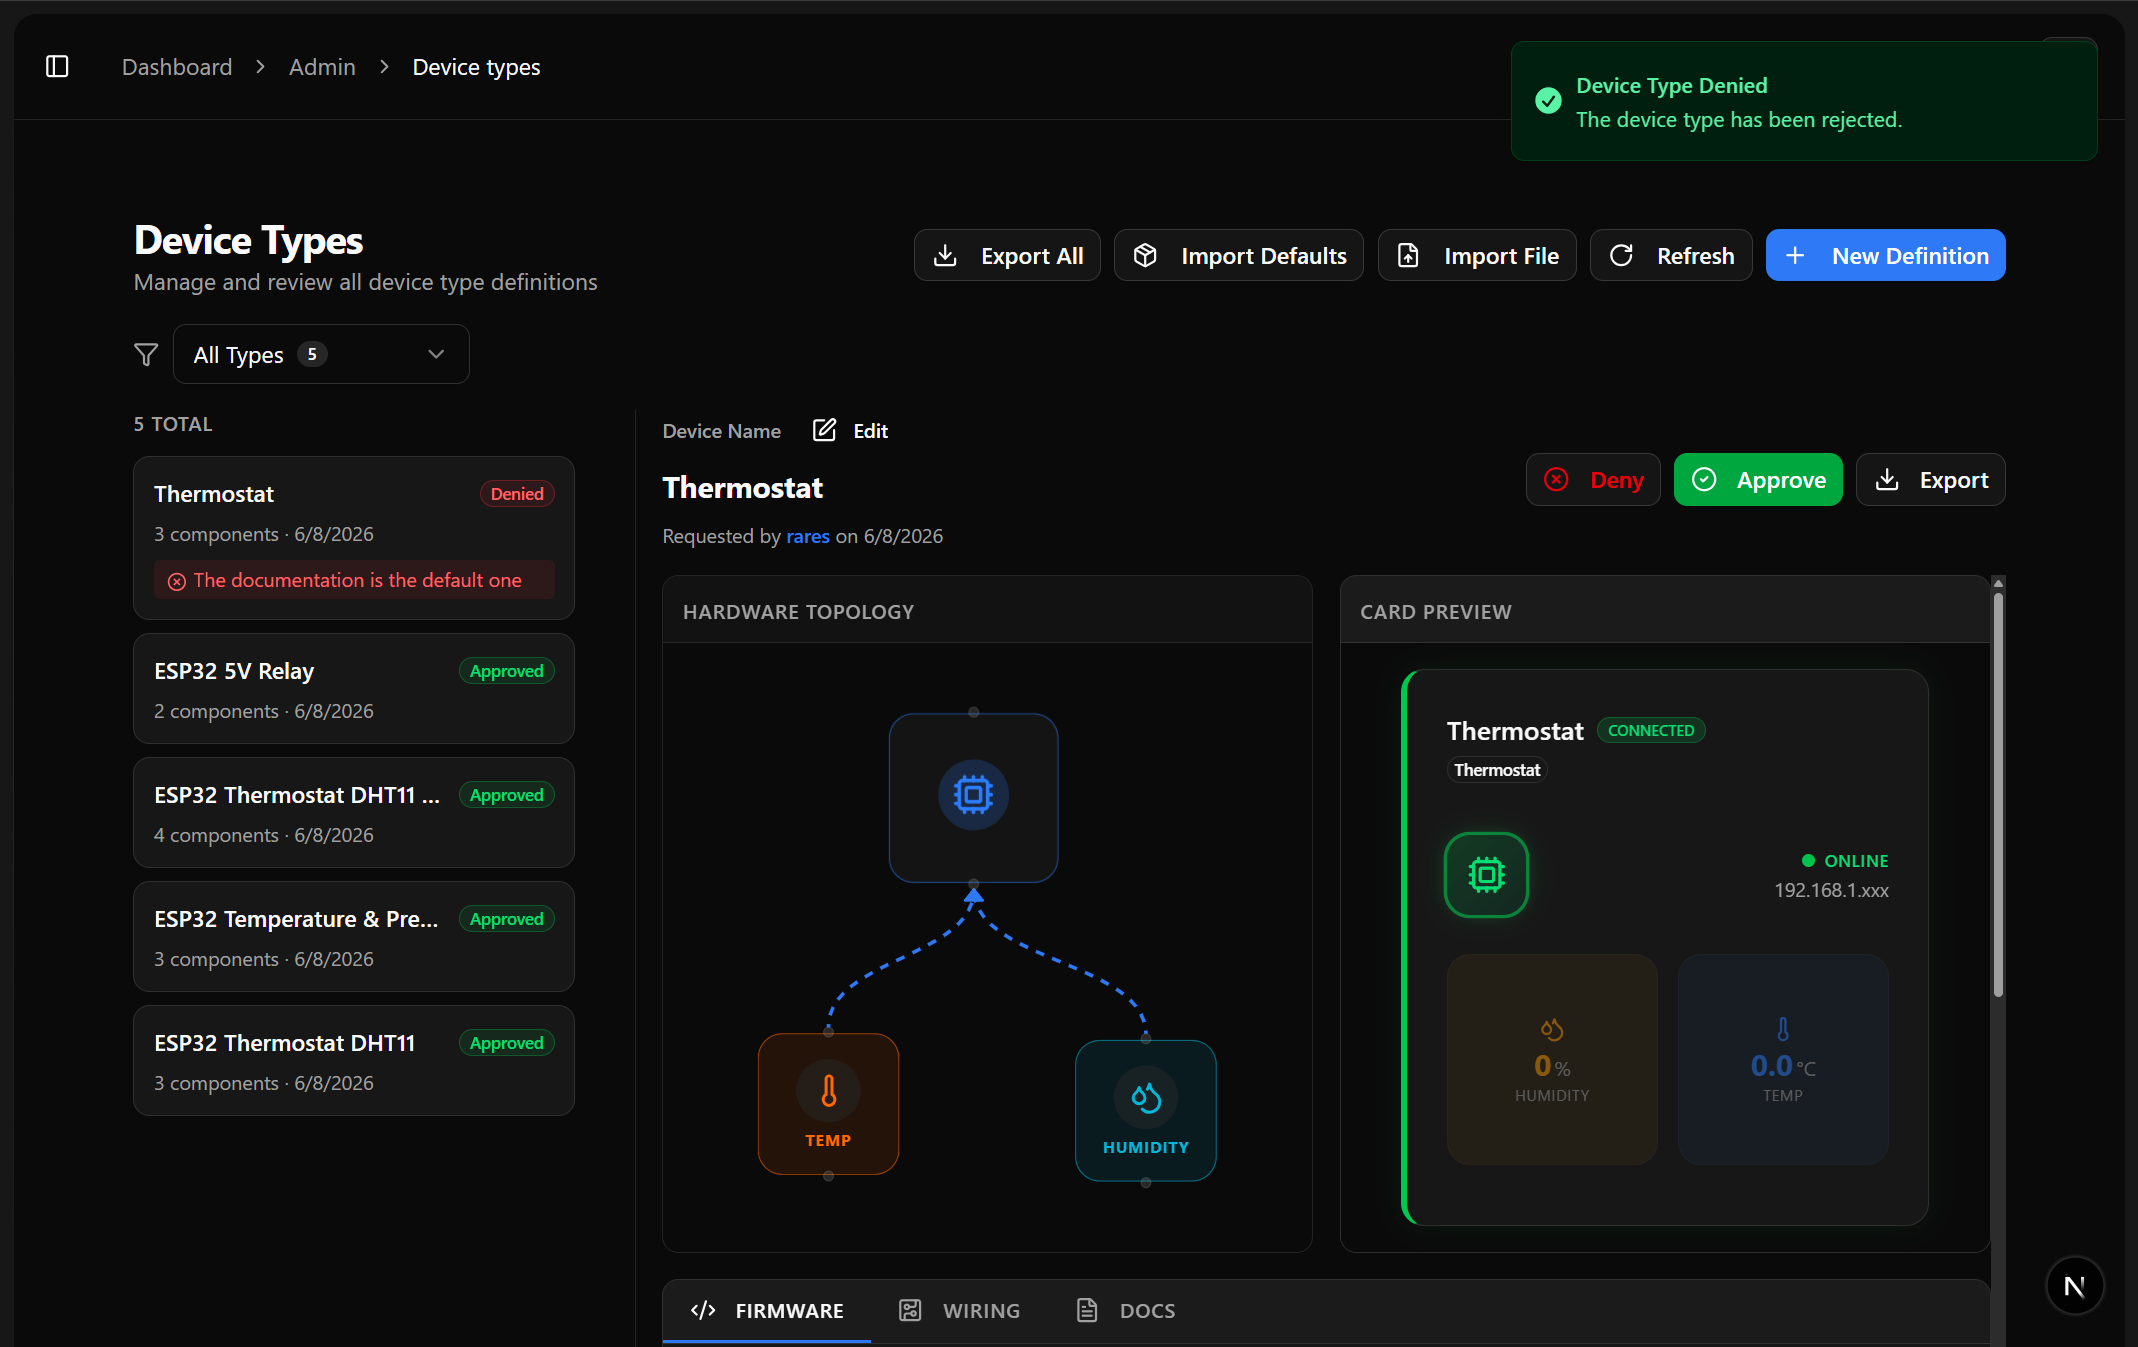
\includegraphics[width=0.95\textwidth]{figuri/admin_approvals.png}
    \caption{Pagina de aprobare a tipurilor de dispozitive propuse de utilizatori (screenshot de adăugat)}
    \label{fig:admin_approvals}
\end{figure}

\subsection{Gestiunea utilizatorilor: \texttt{users/}}
\texttt{app/dashboard/admin/users/page.tsx} afișează un tabel \texttt{Table} (shadcn/ui) cu toți utilizatorii din sistem. Coloanele includ avatar, username, email, rol și un meniu de acțiuni (\texttt{DropdownMenu} cu \texttt{DropdownMenuSub} pentru schimbarea rolului). Filtrul de top oferă o căutare textuală live (controlată local) și un select pentru filtrare după rol. Url-ul acceptă un \texttt{?highlight=<id>} care evidențiază temporar un user — folosit din notificări pentru deep-linking.

\subsection{Camerele, tipurile de dispozitive, debug-ul}
Restul sub-paginilor au design similar. Pe scurt: \texttt{admin/rooms/} face CRUD pe camere folosind \texttt{IconPicker} pentru iconițe (ștergerea unei camere lasă dispozitivele în starea „neasignată" prin \texttt{on\_delete=SET\_NULL}); \texttt{admin/device-types/} listează toate tipurile cu suport pentru import/export JSON și ștergere în bulk a celor respinse; \texttt{admin/debug/} este o pagină de \emph{debugging} unde administratorul poate suprascrie manual starea unui dispozitiv (\texttt{Textarea} cu JSON validat live), forța statusul \texttt{online}/\texttt{offline}/\texttt{error} și trimite comenzi de probă — utilă pentru dezvoltarea UI-ului fără hardware la îndemână.

\section{Recapitulare}
Frontend-ul HomeForge este un Next.js obișnuit, în care complexitatea reală se concentrează în câteva fișiere bine delimitate:
\begin{itemize}
    \item \texttt{apiClient.js} — comunicarea cu API-ul, gestionarea JWT;
    \item \texttt{SmartDeviceCard.tsx} — randarea dinamică a cardurilor și optimistic UI;
    \item \texttt{useDashboardLayout.ts} — layout-ul persistent al dashboard-ului;
    \item \texttt{DeviceUICreator.tsx} — device builder-ul cu graf vizual.
\end{itemize}
Restul codului — sidebar, breadcrumbs, mode toggle, pagini de admin — este aproape integral declarativ, ceea ce reflectă filozofia generală a proiectului: simplitate vizibilă, transparență a fluxului de date.

\chapter{Firmware-ul ESP32 și integrarea hardware}

\section{Alegerea platformei: de ce ESP32}
Tot firmware-ul livrat cu HomeForge este țintit pe familia Espressif ESP32. Decizia se bazează pe patru argumente practice, nu pe vreo afinitate de brand:
\begin{enumerate}
    \item \textbf{Cost.} Modulele ESP32-WROOM-32 (DevKit V1, Figura~\ref{fig:esp32_devkit}) costă aproximativ 5 euro la achiziție unitară, un termen acceptabil pentru un proiect didactic în care studentul probabil va arde măcar o placă învățând.
    \item \textbf{Wi-Fi integrat.} Spre deosebire de Arduino UNO, ESP32 include nativ Wi-Fi (802.11 b/g/n), Bluetooth Low Energy și un dual-core la 240 MHz. Nu este nevoie de niciun \textit{shield} adițional pentru conectarea la LAN.
    \item \textbf{Compatibilitate cu Arduino IDE.} Toolchain-ul ESP-IDF este pentru cei care vor să meargă în profunzime; pentru un demonstrator didactic este suficient framework-ul Arduino-ESP32, cu funcții familiare (\texttt{setup()}, \texttt{loop()}).
    \item \textbf{Comunitate vastă.} Biblioteci precum \texttt{PubSubClient} (pentru MQTT), \texttt{ArduinoJson} (pentru parsing/serializare JSON) și \texttt{DHT} sunt utilizate de zeci de mii de proiecte și au documentație abundentă.
\end{enumerate}

\begin{figure}[htb]
    \centering
    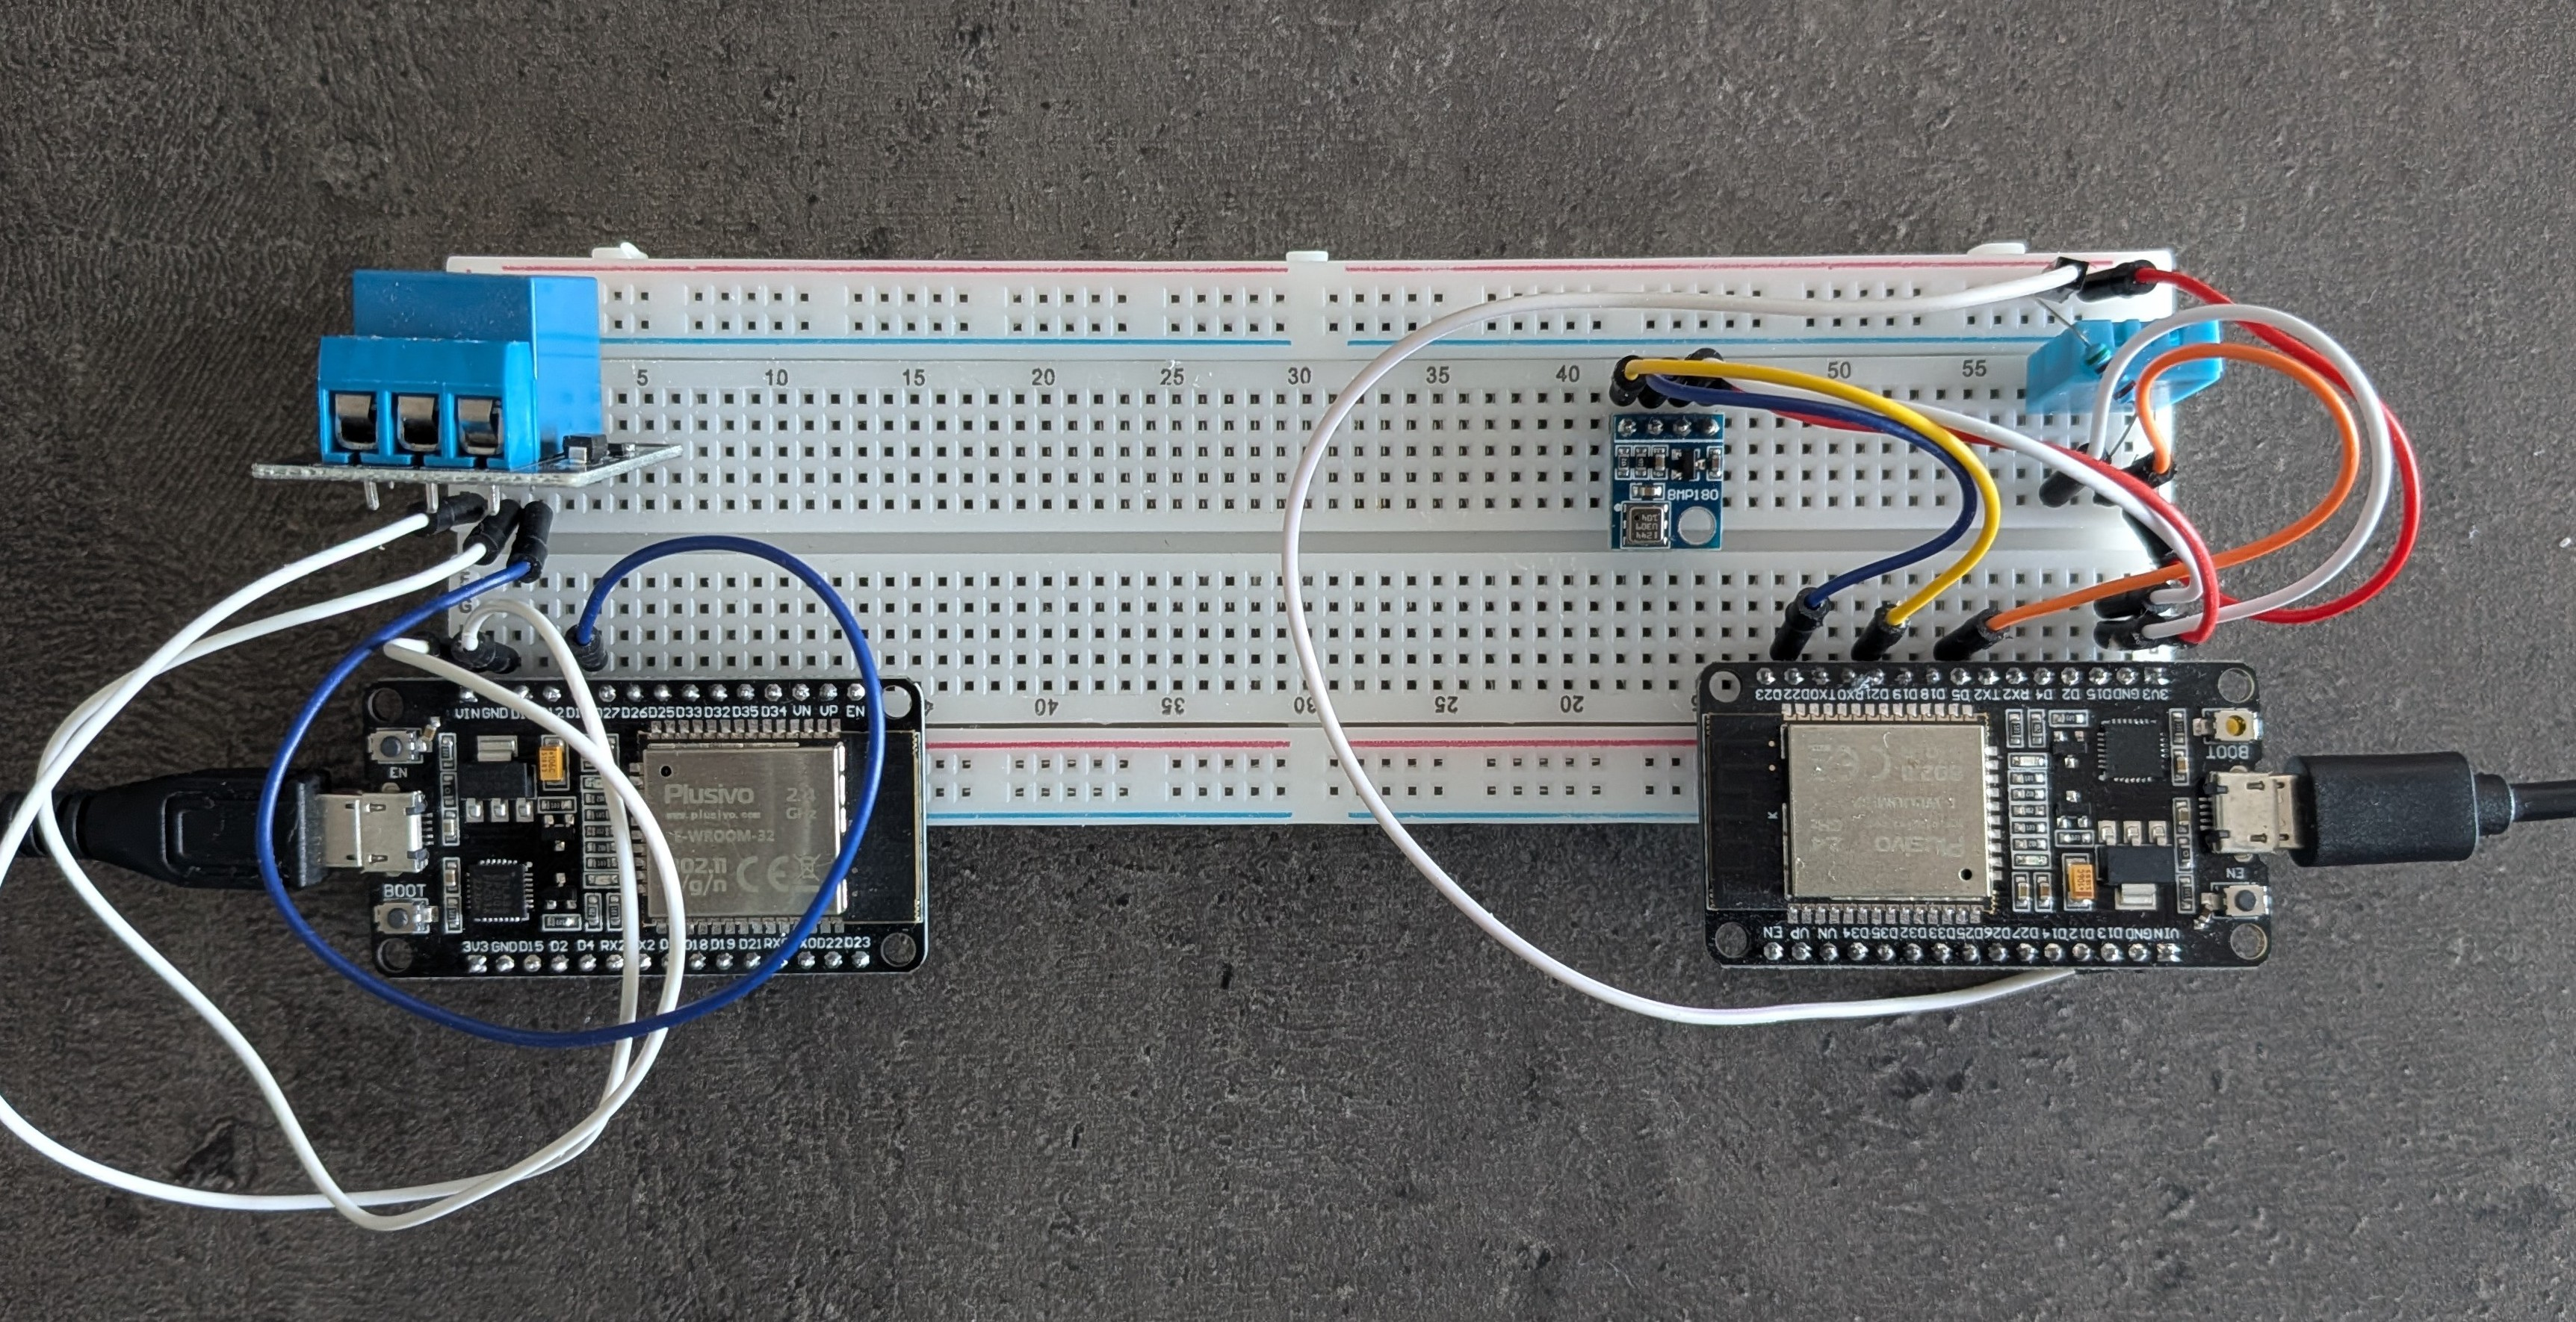
\includegraphics[width=0.7\textwidth]{figuri/esp32_devkit_overview.jpg}
    \caption{Modulul ESP32 DevKit V1 utilizat în prototipurile HomeForge}
    \label{fig:esp32_devkit}
\end{figure}

\section{Anatomia unui sketch HomeForge}
Toate variantele de firmware folosite de HomeForge sunt distribuite \emph{inline} în fișierul fixture \texttt{backend/api/fixtures/default\_device\_types.json}, sub câmpul \texttt{firmware\_code} al fiecărui tip de dispozitiv. Această structurare elimină dependența de un arbore de fișiere separat și permite ca distribuția unui set complet de tipuri (cod sursă, schemă electrică în Markdown și imagini codificate \texttt{base64}) să se reducă la o singură resursă JSON. Pentru a face explicațiile cât mai concrete, exemplele de mai jos provin din varianta \emph{ESP32 5V Relay}. Este singurul template care implementează ambele sensuri: fluxul de telemetrie (publicare de stare) și fluxul invers de comenzi (subscribe + callback). Astfel integrez ambele direcții de comunicație MQTT într-un singur fișier sursă. Pentru fluxurile pur senzoriale (publicare ciclică, fără recepție de comenzi), referințele vor merge către varianta \emph{ESP32 Thermostat DHT11 BMP180}.

\subsection{Variabile de configurare (placeholder-uri)}
Primele linii ale fiecărui sketch conțin trei constante marcate cu placeholder-uri Mustache-like:
\begin{minted}{cpp}
const char* wifi_ssid = "{{WIFI_SSID}}";
const char* wifi_password = "{{WIFI_PASSWORD}}";
const char* server_ip = "{{SERVER_IP}}";
const int mqtt_port = 1883;
\end{minted}
Aceste valori sunt înlocuite în clar de către utilizator înainte de compilare. \texttt{wifi\_ssid} și \texttt{wifi\_password} sunt strict obligatorii: backend-ul refuză să accepte un \texttt{firmware\_code} care nu conține referințele lor. În schimb, \texttt{server\_ip} a devenit \emph{opțional}: dispozitivul poate descoperi singur brokerul prin mDNS, mecanism descris în secțiunea \ref{sec:firmware-mdns}. Validatorul tratează valorile goale (\texttt{""} sau placeholder-ul ne-înlocuit) ca un semnal pentru activarea descoperirii automate, iar instalarea funcționează în acest caz fără ca utilizatorul să caute manual adresa serverului HomeForge.

\subsection{Identitatea dispozitivului: \texttt{deviceMac}}
La pornire, după conectarea la Wi-Fi, sketch-ul citește adresa MAC a interfeței Wi-Fi a cip-ului, o normalizează și se anunță în rețeaua locală prin mDNS:
\begin{minted}{cpp}
void setup_wifi() {
  delay(10);
  Serial.printf("\nConnecting to %s", wifi_ssid);
  WiFi.mode(WIFI_STA);
  WiFi.begin(wifi_ssid, wifi_password);
  while (WiFi.status() != WL_CONNECTED) {
    delay(500);
    Serial.print(".");
  }
  deviceIp  = WiFi.localIP().toString();
  deviceMac = WiFi.macAddress();
  deviceMac.replace(":", "");

  commandTopic = String("homeforge/devices/") + deviceMac + "/command";
  stateTopic   = String("homeforge/devices/") + deviceMac + "/state";

  String hostname = "homeforge-" + deviceMac;
  if (MDNS.begin(hostname.c_str())) {
    Serial.printf("mDNS responder started: %s.local\n", hostname.c_str());
  }
}
\end{minted}
La firmware-urile pur senzoriale, linia \texttt{commandTopic} lipsește (nu există nimic la care să se aboneze), restul fiind identic.
Patru detalii merită semnalate:
\begin{itemize}
    \item \texttt{WiFi.mode(WIFI\_STA)} forțează modul \emph{station-only}, oprind orice activitate de soft-AP rămasă din încercări anterioare;
    \item adresa MAC este formatată implicit de Arduino-ESP32 cu separatori (\texttt{:}); se elimină pentru ca topicul MQTT să fie un singur token alfanumeric, același format pe care îl așteaptă \texttt{mqtt\_listener} pe partea de Django;
    \item topicul \texttt{state} este construit pe toate firmware-urile; topicul \texttt{command} este construit doar de variantele care expun un actuator (\emph{ESP32 5V Relay}), restul fiind pur senzoriale și neavând nevoie să se aboneze la nimic;
    \item adresa MAC servește ca identificator unic la nivel de platformă: un dispozitiv care își schimbă IP-ul își păstrează identitatea către backend.
\end{itemize}

\subsection{Conectarea la broker și subscribe}
Funcția \texttt{reconnect()} este apelată din \texttt{loop()} ori de câte ori clientul \texttt{PubSubClient} pierde legătura. În varianta \emph{ESP32 5V Relay}, funcția înglobează și re-descoperirea brokerului atunci când adresa cache-uită nu mai răspunde:
\begin{minted}{cpp}
void reconnect() {
  while (!client.connected()) {
    if (strlen(mqttServer) == 0) {
      if (!discoverBroker()) { delay(3000); return; }
      client.setServer(mqttServer, mqtt_port);
    }
    Serial.printf("Connecting to MQTT broker %s ...", mqttServer);
    String clientId = "ESP32-Relay-" + deviceMac;
    if (client.connect(clientId.c_str())) {
      Serial.println(" connected!");
      client.subscribe(commandTopic.c_str());   // doar pe firmware-urile cu actuator
      publishState();
    } else {
      Serial.printf(" failed (rc=%d). Retrying in 5s...\n", client.state());
      delay(5000);
      return;
    }
  }
}
\end{minted}
\texttt{clientId} este unic per placă, construit din adresa MAC fără separatori și un prefix care identifică tipul de firmware: \texttt{ESP32-Relay-}, \texttt{ESP32-DHT11-}, \texttt{ESP32-BMP180-} sau \texttt{ESP32-Sensor-} (acesta din urmă pentru varianta combinată DHT11 + BMP180). Aceste prefixe sunt utile la depanare: un \texttt{mosquitto\_sub} pe brokerul HomeForge permite identificarea imediată a tipului de placă care s-a conectat. Imediat după conectare, dispozitivul publică starea curentă prin \texttt{publishState()}. Acest mesaj joacă rolul unui \emph{check-in}: este suficient pentru ca daemon-ul \texttt{mqtt\_listener} să facă auto-binding-ul descris în Capitolul 2. Firmware-urile pur senzoriale au aceeași structură, dar omit linia \texttt{client.subscribe(...)}: neavând actuator, nu se abonează la niciun topic de comandă.

\subsection{Telemetria: \texttt{publishState()}}
Funcția care construiește mesajul de stare folosește \texttt{ArduinoJson} pentru a serializa un document static. Pentru varianta \emph{ESP32 5V Relay}, mesajul publicat conține valoarea actuatorului (\texttt{relay\_1}), un eventual \emph{echo} către cheia dinamică folosită în comanda care a generat starea curentă și câmpurile auxiliare \texttt{ip} / \texttt{mac}:
\begin{minted}{cpp}
void publishState() {
  if (!client.connected()) return;

  StaticJsonDocument<256> doc;
  doc["ip"]  = deviceIp;
  doc["mac"] = deviceMac;
  doc[VAR_RELAY] = relayState;
  if (lastControlKey.length() > 0) {
    doc[lastControlKey] = relayState;   // trimite înapoi cheia dinamică
  }

  char buffer[256];
  serializeJson(doc, buffer);
  client.publish(stateTopic.c_str(), buffer);
}
\end{minted}
Mecanismul \emph{echo} acoperă cazul în care device builder-ul a generat o cheie dinamică pentru widget (de exemplu \texttt{switch-1780830762843}): firmware-ul reține ultima cheie primită în \texttt{lastControlKey} și o include în mesajul de stare alături de \texttt{relay\_1}, astfel încât interfața să vadă confirmarea pe identificatorul exact pe care l-a folosit la trimitere. Termostatele senzoriale (\emph{DHT11}, \emph{BMP180}, \emph{DHT11 + BMP180}) folosesc același tipar, dar populează câmpurile relevante pentru senzorii lor (\texttt{VAR\_TEMP}, \texttt{VAR\_HUMID}, \texttt{VAR\_PRESSURE}, după caz), fără \texttt{VAR\_RELAY} (nu au actuator). \texttt{StaticJsonDocument} cu dimensiune fixă alocă memoria în stivă, nu pe heap, ceea ce este recomandat pe microcontrolere unde fragmentarea heap-ului poate cauza eșecuri intermitente după ore de funcționare. Câmpurile \texttt{ip} și \texttt{mac} sunt incluse în payload chiar dacă brokerul le-ar putea infera din topic, fiind utile pentru auto-binding-ul descris în Capitolul 2, atunci când backend-ul nu cunoaște încă adresa MAC. Constantele de denumire a câmpurilor sunt declarate la începutul fiecărui sketch:
\begin{minted}{cpp}
const char* VAR_RELAY    = "relay_1";    // doar în ESP32 5V Relay
const char* VAR_TEMP     = "temperature";
const char* VAR_HUMID    = "humidity";
const char* VAR_PRESSURE = "pressure";
\end{minted}
Aceste nume sunt cele „standard", pe care \texttt{mqtt\_listener.map\_standard\_key()} le translatează către cheile dinamice ale widget-urilor.

\subsection{Recepția comenzilor: \texttt{callback()}}
Callback-ul \texttt{PubSubClient} este apelat de fiecare dată când brokerul publică un mesaj pe topicul la care firmware-ul s-a abonat. Implementarea concretă din \emph{ESP32 5V Relay} iterează peste cheile documentului JSON și acceptă, pe lângă \texttt{relay\_1}, orice identificator care începe cu prefixul \texttt{switch-} (folosit de device builder atunci când utilizatorul nu redenumește manual controlul). Parser-ul tolerează trei reprezentări pentru valoarea booleană (boolean nativ, string \texttt{"true"}, \texttt{"on"}, \texttt{"1"} și întreg), pentru a fi compatibil cu diferitele stiluri de payload pe care le poate genera UI-ul:
\begin{minted}{cpp}
void callback(char* topic, byte* payload, unsigned int length) {
  String message;
  for (unsigned int i = 0; i < length; i++) {
    message += (char)payload[i];
  }
  Serial.print("Command received: ");
  Serial.println(message);

  StaticJsonDocument<256> doc;
  if (deserializeJson(doc, message)) return;

  JsonObject root = doc.as<JsonObject>();
  for (JsonPair kv : root) {
    String key = kv.key().c_str();
    if (key == VAR_RELAY || key.startsWith("switch-")) {
      lastControlKey = key;
      if (kv.value().is<bool>()) {
        relayState = kv.value().as<bool>();
      } else if (kv.value().is<const char*>()) {
        String val = kv.value().as<String>();
        val.toLowerCase();
        relayState = (val == "true" || val == "on" || val == "1");
      } else if (kv.value().is<int>()) {
        relayState = kv.value().as<int>() == 1;
      }
      break;
    }
  }

  digitalWrite(RELAY_PIN, relayState ? HIGH : LOW);

  preferences.begin("state", false);
  preferences.putBool("relay", relayState);
  preferences.end();

  publishState();
}
\end{minted}
Trei detalii merită observate. Primul: variabila \texttt{lastControlKey} reține identificatorul exact cu care a venit ultima comandă, pentru ca \texttt{publishState()} să poată face \emph{echo} înapoi pe aceeași cheie dinamică (mecanism prezentat în subsecțiunea anterioară). Al doilea: după acționarea releului, starea este persistată în memoria nevolatilă a ESP32 (\texttt{Preferences}, namespace \texttt{state}), astfel încât după o reală cădere de tensiune dispozitivul revine în aceeași stare la pornire. Al treilea: \texttt{publishState()} este apelat imediat după execuție, închizând bucla de feedback: backend-ul primește confirmarea că operația a fost realizată și actualizează \texttt{current\_state} în baza de date, iar frontend-ul preia noua valoare la următoarea iterație de \texttt{refetchInterval} (3 secunde).

\subsection{Bucla principală}
\texttt{loop()} este structurată în trei pași: servirea serverului HTTP de fallback (\texttt{server.handleClient()} pentru endpoint-ul \texttt{/config}), asigurarea conexiunii MQTT prin \texttt{reconnect()} și o secvență ciclică de eșantionare la fiecare câteva secunde. Pentru \emph{ESP32 5V Relay}, partea ciclică se limitează la republicarea stării actuatorului (nu există senzori de citit); pentru firmware-urile de termostat, citirea senzorilor este izolată într-o funcție \texttt{readSensors()} apelată din bucla principală. Schema buclei pentru varianta \emph{ESP32 Thermostat DHT11 BMP180}:
\begin{minted}{cpp}
void loop() {
  server.handleClient();
  if (!client.connected()) {
    reconnect();
  }
  client.loop();

  unsigned long now = millis();
  if (now - lastMsg > interval) {
    lastMsg = now;
    readSensors();
    publishState();
  }
}

void readSensors() {
  float newT = dht.readTemperature();
  float newH = dht.readHumidity();
  float newP = bmp.readPressure();

  if (!isnan(newT) && !isnan(newH)) {
    humidity = newH;
    // Aplică corecția de toleranță DHT11.
    temperature = (DHT11_ERROR < 0) ? newT + DHT11_ERROR : newT - DHT11_ERROR;
    if (!isnan(newP)) pressure = newP / 100.0;   // Pa în hPa
  } else {
    Serial.println("Failed to read from DHT11/BMP180 sensor!");
  }
}
\end{minted}
Constanta \texttt{interval = 5000} (5 secunde) este sincronizată cu pragul din \texttt{mqtt\_listener.check\_offline\_devices()} (30 de secunde): primim 6 oportunități de heartbeat ratate înainte ca dispozitivul să fie declarat offline. Pe DHT11, citirile prea frecvente nu sunt fiabile (senzorul are nevoie de cel puțin o secundă între eșantioane), deci intervalul de 5 secunde oferă o marjă confortabilă. Verificarea \texttt{!isnan(newT) \&\& !isnan(newH)} reține valorile vechi atunci când o citire eșuează intermitent, iar constanta \texttt{DHT11\_ERROR} aplică o corecție de offset pentru a compensa eroarea sistematică observată la lotul de DHT11 folosit. Presiunea barometrică este convertită din Pascali (unitate brută a BMP180) în hectopascali (\texttt{hPa}), unitatea uzuală în meteorologie.

\section{Descoperirea automată a brokerului prin mDNS}
\label{sec:firmware-mdns}
Una dintre operațiunile mai puțin elegante în implementarea inițială era cerința ca utilizatorul să cunoască adresa IP a serverului HomeForge înainte de compilare. Pentru rețelele în care IP-ul serverului este atribuit dinamic prin DHCP, această cerință devenea o sursă recurentă de probleme: o singură reasignare DHCP forța re-flash-area tuturor dispozitivelor. Versiunea curentă rezolvă acest aspect prin introducerea unui mecanism de descoperire automată bazat pe Multicast DNS (mDNS) și DNS-Based Service Discovery (DNS-SD), conform RFC 6762 \cite{rfc_mdns} și RFC 6763 \cite{rfc_dnssd}.

\subsection{Principiul de funcționare}
mDNS permite rezolvarea numelor DNS pe segmentul local de rețea fără a depinde de un server DNS centralizat, prin trimiterea de pachete UDP către adresa de multicast \texttt{224.0.0.251} (IPv4), pe portul 5353. DNS-SD extinde acest mecanism cu o convenție pentru descoperirea serviciilor: un client interesat de un serviciu de tipul „MQTT peste TCP" interoghează numele rezervat \texttt{\_mqtt.\_tcp.local}, iar furnizorii de serviciu răspund cu o înregistrare SRV care indică gazda și portul efectiv. HomeForge folosește această convenție prin daemon-ul Avahi care rulează în containerul backend (acolo unde topologia de rețea o permite, vezi Capitolul 5), publicând în mod continuu un record \texttt{\_mqtt.\_tcp} cu portul 1883.

\subsection{Ierarhia celor trei niveluri de descoperire}
Firmware-ul ESP32 încearcă să identifice brokerul printr-o secvență de trei mecanisme, în ordinea priorității:

\begin{enumerate}
    \item \textbf{Override manual prin \texttt{server\_ip}.} Dacă utilizatorul a substituit explicit adresa serverului la momentul compilării, dispozitivul se conectează direct, fără descoperire. Modul este util pentru topologii fixe sau pentru sisteme unde mDNS nu este disponibil.
    \item \textbf{Cache local în memorie nevolatilă (NVS).} La fiecare conectare reușită, firmware-ul salvează adresa brokerului în NVS folosind biblioteca \texttt{Preferences}. La un \texttt{reboot} ulterior, reconectarea este aproape instantanee fiindcă cache-ul este consultat înainte de a iniția o nouă interogare multicast.
    \item \textbf{Interogare mDNS / DNS-SD.} Atunci când \texttt{server\_ip} este gol și cache-ul lipsește sau este invalid, firmware-ul folosește biblioteca \texttt{ESPmDNS} pentru a interoga \texttt{\_mqtt.\_tcp} pe segmentul de rețea. Funcția \texttt{discoverBroker()} încearcă până la trei interogări consecutive (cu timeout scurt) și acceptă primul răspuns valid:
\end{enumerate}

\begin{minted}{cpp}
bool discoverBroker() {
  Serial.println("Discovering HomeForge broker via mDNS...");
  for (int attempt = 0; attempt < 3; attempt++) {
    int n = MDNS.queryService(MDNS_SERVICE, MDNS_PROTO);
    if (n > 0) {
      IPAddress ip = MDNS.address(0);
      String found = ip.toString();
      if (found != "0.0.0.0") {
        strncpy(mqttServer, found.c_str(), sizeof(mqttServer) - 1);
        saveBroker(found);
        Serial.printf("Broker found: %s\n", mqttServer);
        return true;
      }
    }
    delay(1000);
  }
  Serial.println("Broker not found (will retry / use /config fallback).");
  return false;
}
\end{minted}
\texttt{mqttServer} este un buffer de caractere global (umplut prin \texttt{strncpy}), iar \texttt{saveBroker(found)} apelează API-ul \texttt{Preferences} pentru a persista adresa descoperită în memoria nevolatilă a ESP32, pentru reutilizare la următorul boot.

Dacă toate cele trei niveluri eșuează (situație rară, dar plauzibilă atunci când serverul nu rulează încă sau este pe altă subrețea), dispozitivul activează un al patrulea mecanism de rezervă: pornește un server HTTP pe portul 80 și acceptă o cerere \texttt{POST /config} cu adresa brokerului. Utilizatorul deschide în browser pagina dispozitivului și introduce adresa manual, fără a fi necesar un reflash.

\subsection{Anunțarea propriei identități prin mDNS}
Pe lângă consumarea înregistrărilor mDNS, fiecare dispozitiv își publică și propria identitate, sub un nume derivat din adresa MAC: \texttt{esp32-<MAC>.local}. Astfel, administratorul rețelei locale poate accesa dispozitivul prin nume DNS, fără a căuta IP-ul în interfața de administrare a router-ului. Apelul \texttt{MDNS.begin(hostname)} se face imediat după conectarea la Wi-Fi, în secvența standard de inițializare.
Setul predefinit conține patru tipuri de dispozitive ESP32, toate stocate inline în \texttt{backend/api/fixtures/default\_device\_types.json} și importate automat la apelul \texttt{POST /api/device-types/import-defaults/} în prima sesiune cu administratorul. Fiecare intrare conține integral codul firmware Arduino, schema electrică (text Markdown + imagine \texttt{base64}), documentația și definiția vizuală a cardului, totul într-un singur obiect JSON, fără referințe către fișiere externe.

Cele patru variante împart o singură categorie funcțională clară. \textbf{ESP32 5V Relay} este singurul template care expune un actuator: un releu controlat de \texttt{RELAY\_PIN = GPIO 14}, redat în interfață printr-un widget \texttt{TOGGLE} a cărui variabilă (\texttt{relay\_1} sau un identificator generat dinamic care începe cu prefixul \texttt{switch-}) este transmisă bidirecțional, atât în publicările de stare cât și în comenzile primite de la backend. Celelalte trei variante sunt strict senzoriale: publică telemetrie ciclică, fără a se abona la topicul de comandă și fără a implementa un \texttt{callback} de recepție.

\textbf{ESP32 Thermostat DHT11} folosește un senzor DHT11 (temperatură + umiditate) conectat la \texttt{DHTPIN = GPIO 5} și expune două widget-uri: \texttt{TEMPERATURE} și \texttt{HUMIDITY}. \textbf{ESP32 Temperature \& Pressure BMP180} folosește un senzor BMP180 pe magistrală I2C (\texttt{SDA = GPIO 21}, \texttt{SCL = GPIO 22}, valorile implicite Wire ale ESP32), publicând temperatura măsurată de BMP-ul însuși și presiunea barometrică în două widget-uri \texttt{TEMPERATURE} și \texttt{PRESSURE}. \textbf{ESP32 Thermostat DHT11 BMP180} combină cele două: DHT11 pe GPIO 5 și BMP180 pe magistrala I2C standard, publicând trei valori (temperatură, umiditate și presiune) în trei widget-uri corespunzătoare.

Cheile cu care fiecare firmware publică datele pe broker sunt constantele \texttt{VAR\_TEMP = "temperature"}, \texttt{VAR\_HUMID = "humidity"}, \texttt{VAR\_PRESSURE = "pressure"} și \texttt{VAR\_RELAY = "relay\_1"}. Daemon-ul \texttt{mqtt\_listener} de pe partea de backend mapează aceste nume canonice către identificatorii dinamici generați de device builder pentru fiecare widget al cardului, astfel încât reorganizarea widget-urilor în UI nu impune reflash-area firmware-ului.

Pentru fiecare variantă, schema electrică este distribuită ca imagine \texttt{base64} în câmpul \texttt{wiring\_diagram\_base64} al obiectului JSON, însoțită opțional de o descriere textuală în \texttt{wiring\_diagram\_text}. Schema electrică minimală pentru varianta \emph{ESP32 5V Relay} este sintetizată în Tabelul \ref{tab:esp32_relay_pinout}, iar montajele pe breadboard ale tuturor celor patru variante sunt arătate în Figura \ref{fig:wiring_diagrams}:
\begin{table}[htb]
    \centering
        \renewcommand{\arraystretch}{1.2}
    \small
    \begin{tabular}{|l|l|l|l|}
        \hline
        \textbf{Modul} & \textbf{Pin} & \textbf{ESP32} & \textbf{Descriere} \\ \hline
        Releu & VCC & 5V & Alimentare 5 V \\ \hline
        Releu & GND & GND & Masă \\ \hline
        Releu & IN  & GPIO 14 & Semnal de control (\texttt{RELAY\_PIN}) \\ \hline
    \end{tabular}
    \caption{Conexiunile pinilor pentru tipul \emph{ESP32 5V Relay}}
    \label{tab:esp32_relay_pinout}
\end{table}

\begin{figure}[htb]
    \centering
    \begin{subfigure}[t]{0.48\textwidth}
        \centering
        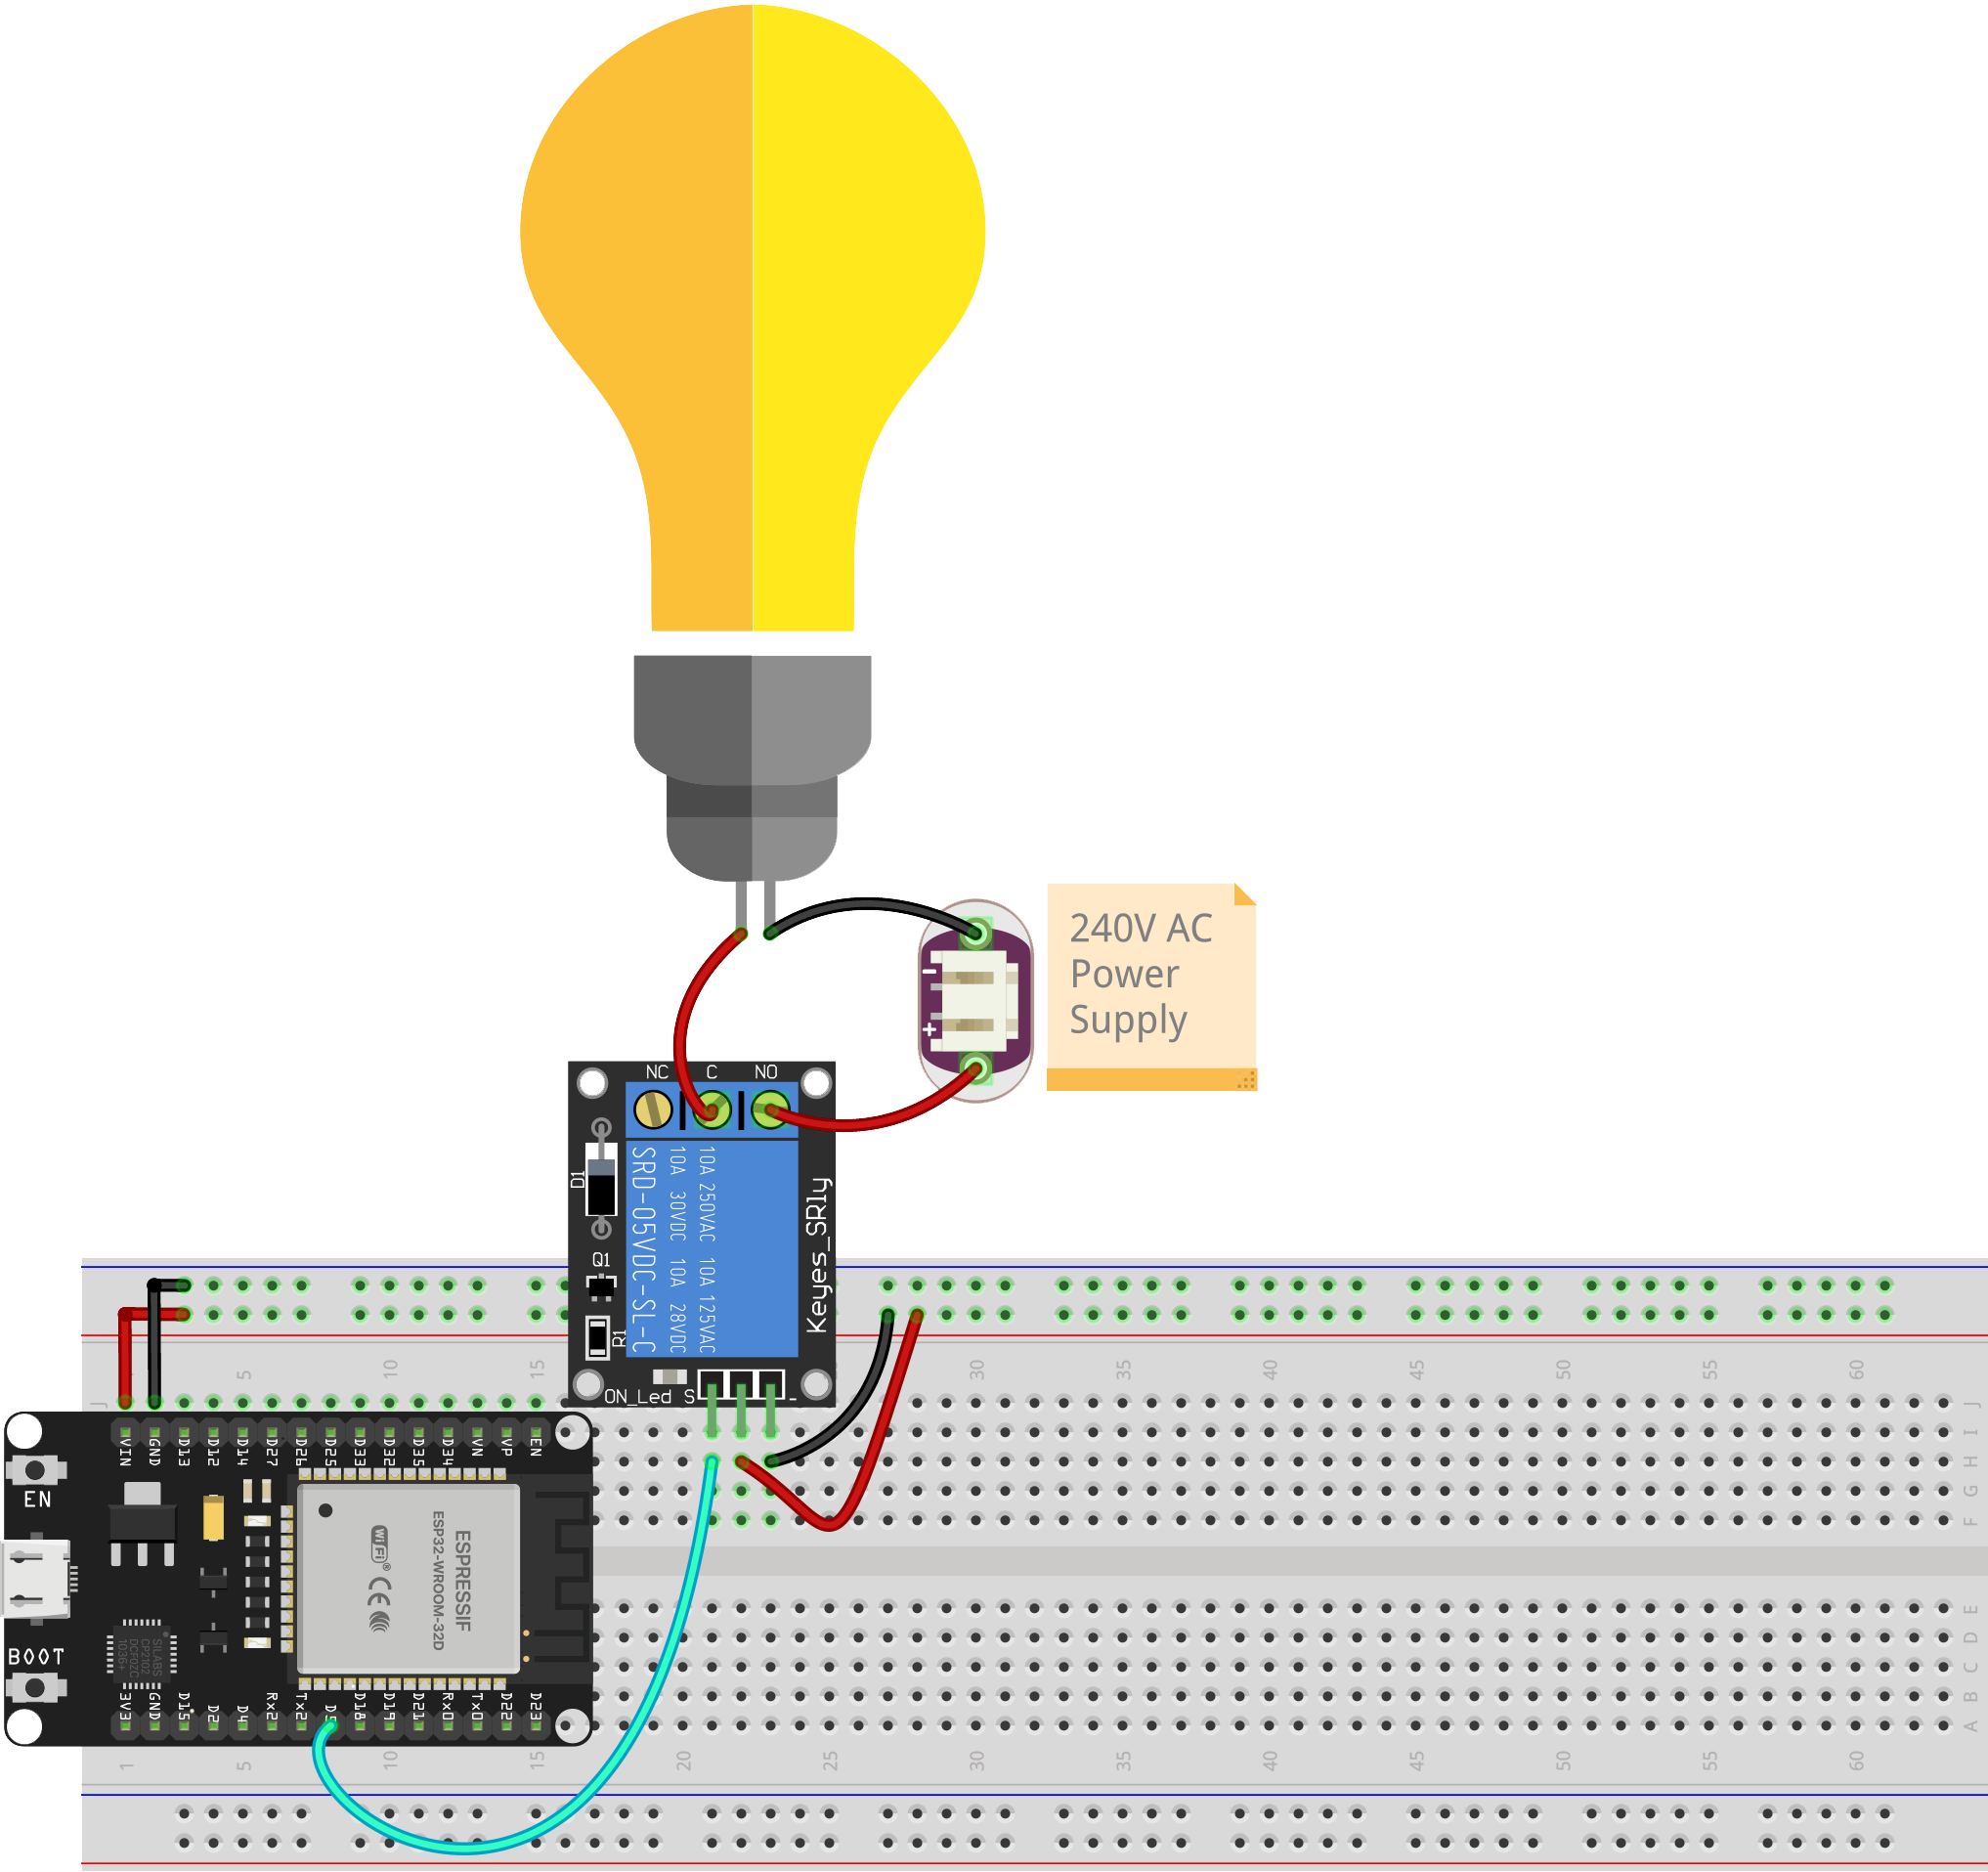
\includegraphics[width=\linewidth]{figuri/breadboard_esp32_relay.png}
        \caption{ESP32 5V Relay}
        \label{fig:wiring_relay}
    \end{subfigure}\hfill
    \begin{subfigure}[t]{0.48\textwidth}
        \centering
        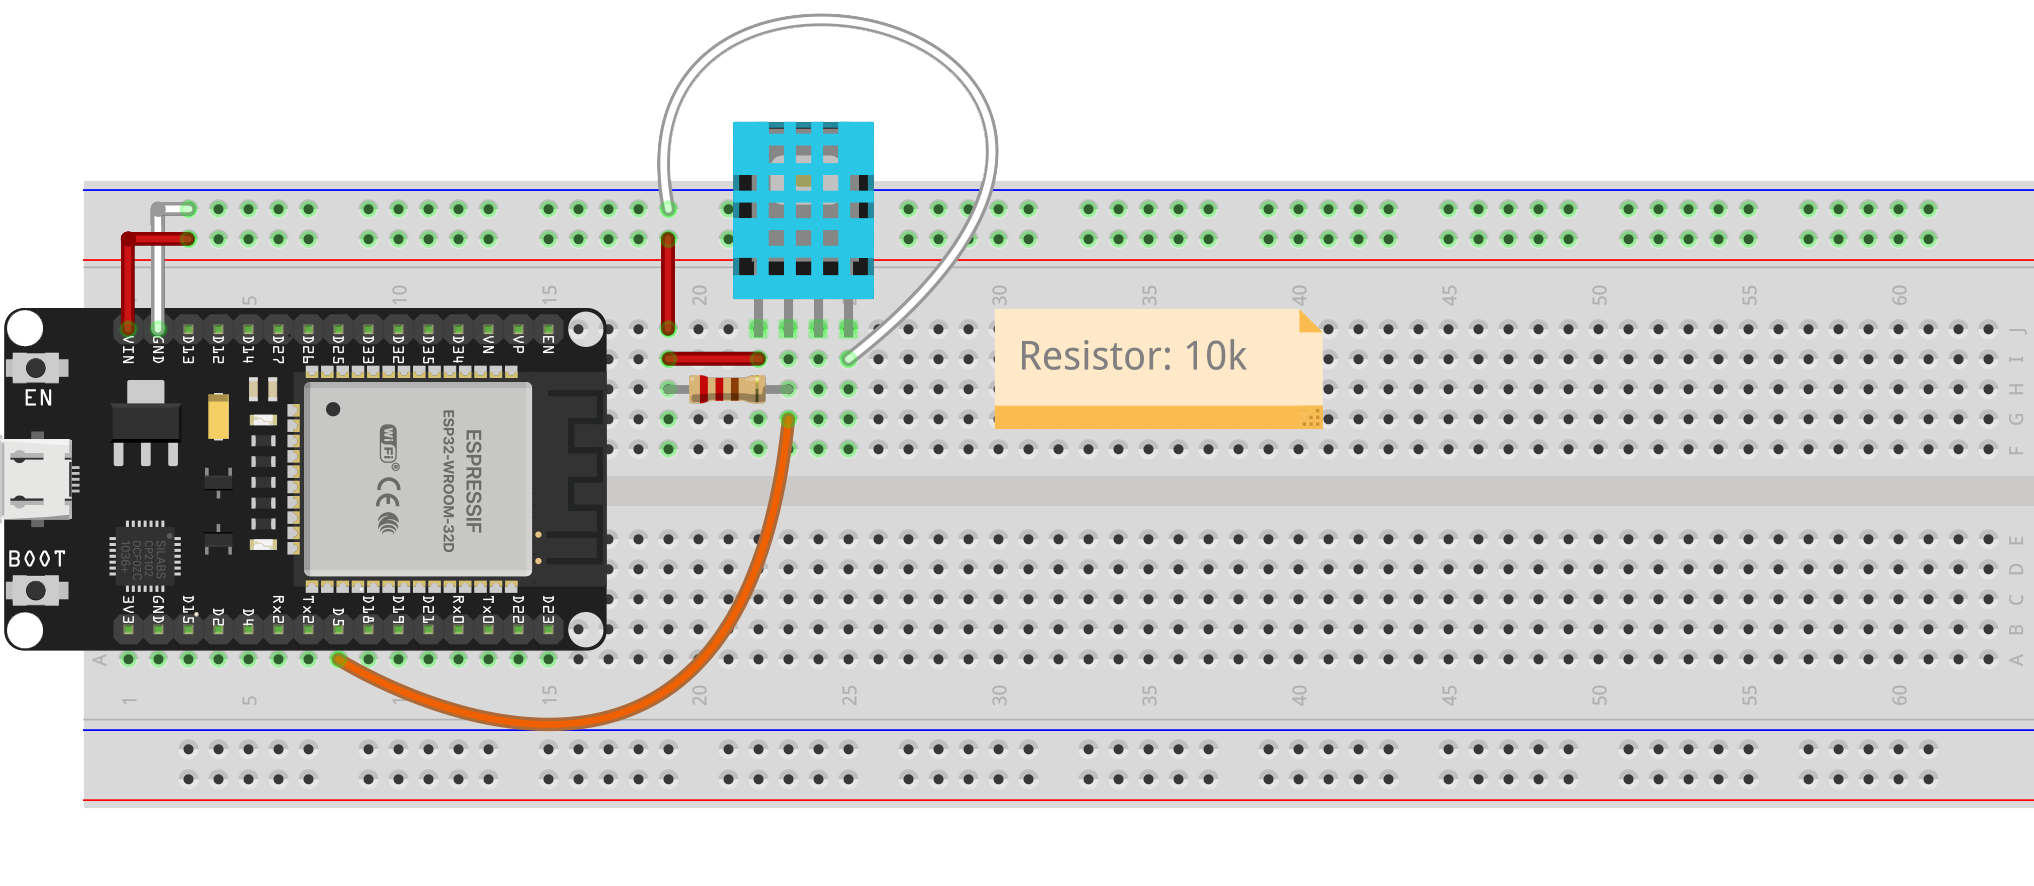
\includegraphics[width=\linewidth]{figuri/breadboard_esp32_thermostat_dht11.png}
        \caption{ESP32 Thermostat DHT11}
        \label{fig:wiring_dht11}
    \end{subfigure}

    \vspace{0.6em}

    \begin{subfigure}[t]{0.48\textwidth}
        \centering
        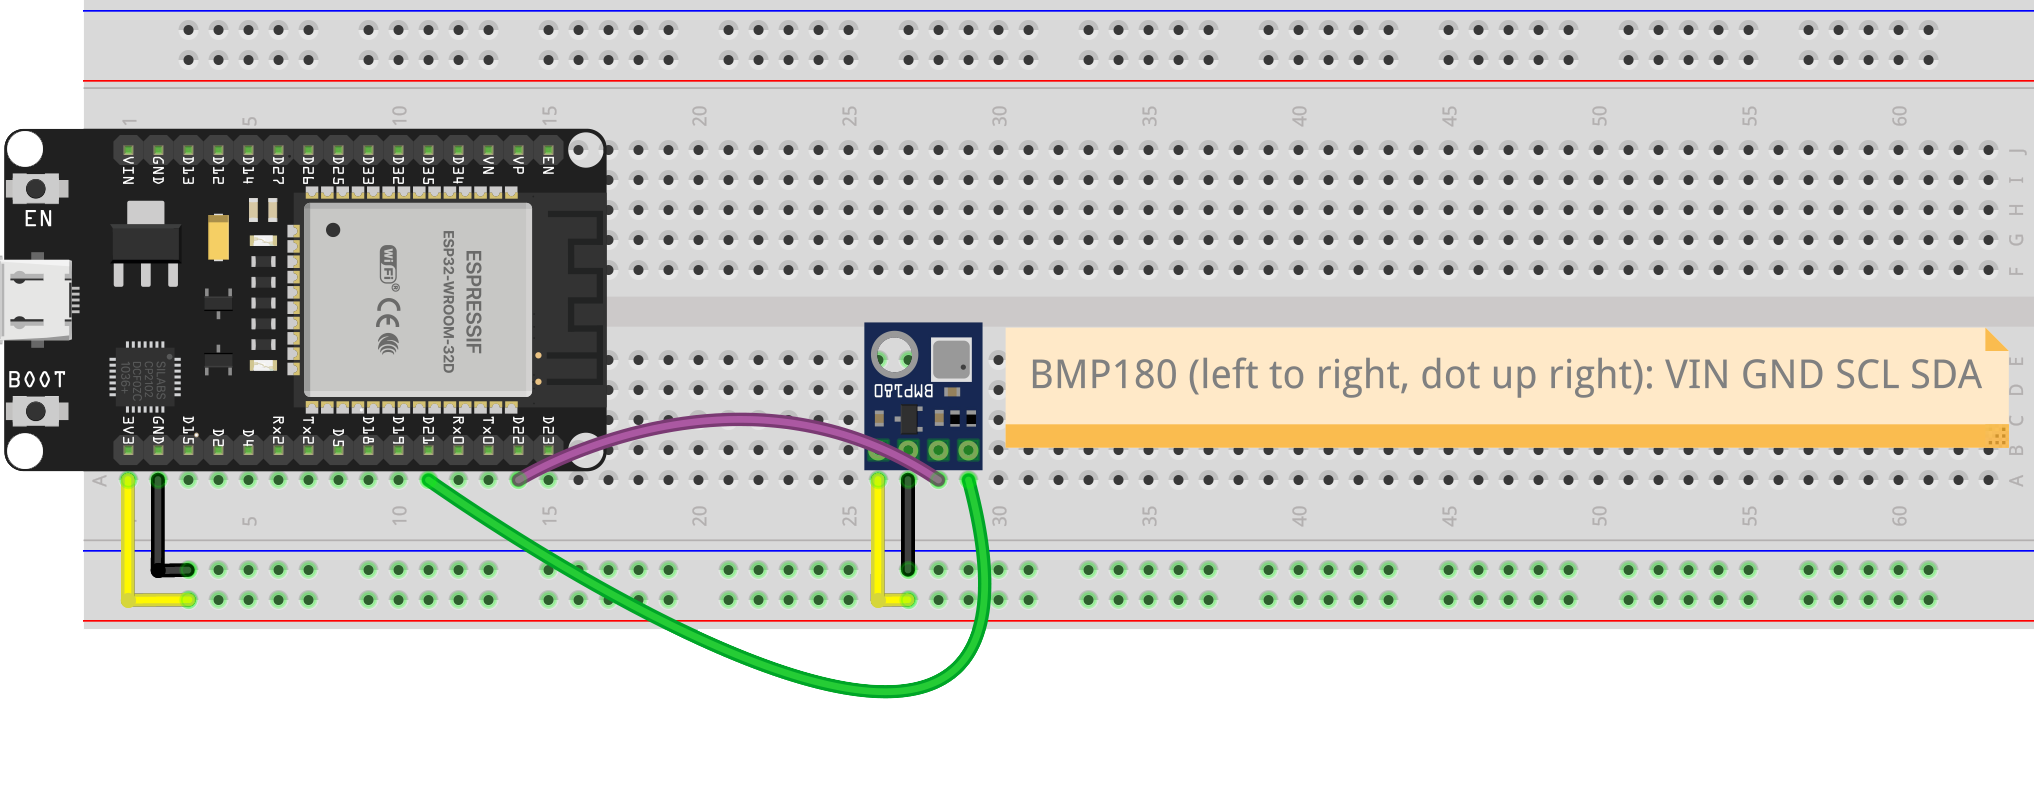
\includegraphics[width=\linewidth]{figuri/breadboard_esp32_thermostat_bmp180.png}
        \caption{ESP32 Temperature \& Pressure BMP180}
        \label{fig:wiring_bmp180}
    \end{subfigure}\hfill
    \begin{subfigure}[t]{0.48\textwidth}
        \centering
        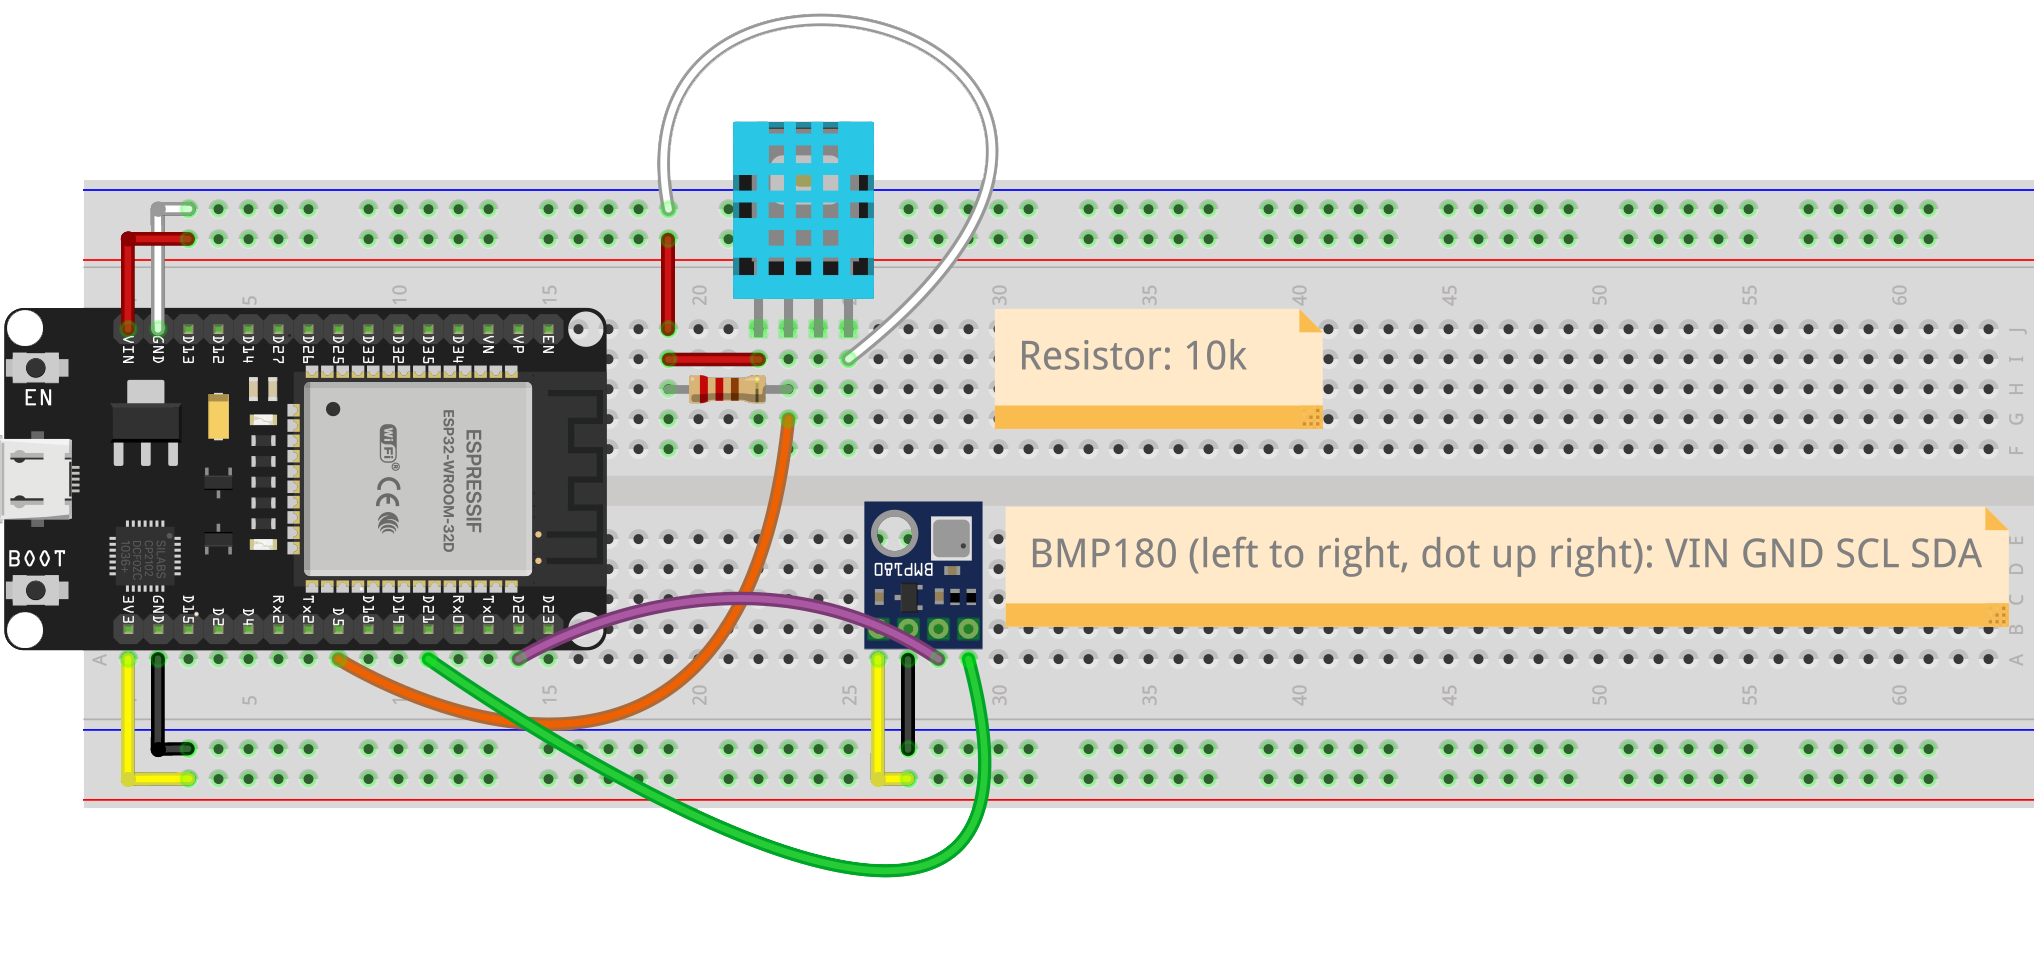
\includegraphics[width=\linewidth]{figuri/breadboard_esp32_thermostat_dht11_bmp180.png}
        \caption{ESP32 Thermostat DHT11 + BMP180}
        \label{fig:wiring_dht11_bmp180}
    \end{subfigure}
    \caption{Schemele de conexiuni (breadboard) ale celor patru tipuri de dispozitive predefinite: releul 5V comandând un consumator (a), termostatul cu DHT11 (b), modulul de temperatură și presiune BMP180 pe I2C (c) și varianta combinată DHT11 + BMP180 (d).}
    \label{fig:wiring_diagrams}
\end{figure}

\FloatBarrier
\section{Bibliotecile Arduino utilizate}
Pentru a compila firmware-urile, mediul Arduino IDE folosește mai multe biblioteci. O parte sunt incluse automat cu pachetul ESP32 Arduino Core de la Espressif: \texttt{WiFi.h} pentru conectarea Wi-Fi, \texttt{ESPmDNS.h} pentru descoperirea automată a brokerului, \texttt{Preferences.h} pentru cache-ul persistent al adresei brokerului în memoria nevolatilă, \texttt{WebServer.h} pentru endpoint-ul de fallback \texttt{/config} și \texttt{Wire.h} pentru comunicarea I2C. Restul se instalează prin \emph{Library Manager}: \texttt{PubSubClient} (Nick O'Leary, client MQTT cu suport pentru QoS 0 și 1), \texttt{ArduinoJson} (Benoit Blanchon, parsing și serializare JSON cu documente alocate static), \texttt{DHT sensor library} (Adafruit, folosită în firmware-urile cu DHT11) și \texttt{Adafruit BMP085 Library} (Adafruit, compatibilă cu BMP180). Pachetul ESP32 Arduino Core se adaugă în Arduino IDE prin \emph{File → Preferences → Additional Boards Manager URLs}, cu URL-ul oficial \texttt{https://espressif.github.io/arduino-esp32/package\_esp32\_index.json}.

\section{Limitări ale implementării curente}
Pentru claritate, enumăr aici ce nu este implementat în firmware-ul curent. Nu folosesc task-uri FreeRTOS create explicit: bucla \texttt{loop()} împreună cu \texttt{PubSubClient.loop()} acoperă volumul actual de logică. Nu există un \texttt{Captive Portal} pentru configurarea Wi-Fi la prima pornire, SSID-ul și parola fiind înlocuite direct în cod prin placeholder-uri. Comunicarea MQTT nu folosește TLS, ceea ce este acceptabil într-un LAN privat, dar pentru un deployment de producție ar trebui adăugate certificate și \texttt{WiFiClientSecure}. Actualizarea OTA nu este implementată, re-flash-area făcându-se prin USB-UART. Niciuna dintre aceste limitări nu împiedică utilizarea curentă a platformei și sunt menționate ca direcții posibile de extindere.
\chapter{Deployment, rulare și testare}

\section{Cele două moduri de rulare}
Pentru fluxul de zi cu zi, HomeForge poate fi pornit în două moduri distincte, ambele incluse explicit în repository: un mod \emph{nativ} pentru dezvoltare locală (scriptul \texttt{dev.sh}) și un mod \emph{containerizat} pentru deployment reproductibil (Docker + Docker Compose). Diferența nu este cosmetică: în modul nativ, backend-ul rulează pe gazdă fără broker MQTT (utilizatorul trebuie să aibă Mosquitto instalat local sau să folosească un broker remote), iar în modul containerizat brokerul este pornit automat în același container cu Django.

\subsection{Modul de dezvoltare locală}
Scriptul \texttt{./dev.sh} pornește, în paralel, backend-ul și frontend-ul. Are trei subcomenzi:
\begin{minted}{bash}
./dev.sh             # Pornește atât backend cât și frontend
./dev.sh backend     # Doar backend (Django pe :8000)
./dev.sh frontend    # Doar frontend (Next.js pe :3000)
\end{minted}
La pornirea backend-ului, scriptul activează automat un \texttt{venv} dacă există (linia \texttt{source venv/bin/activate}) și rulează \texttt{python manage.py runserver 0.0.0.0:8000}. Pentru frontend, lansează \texttt{npm run dev}, care la rândul său invocă Next.js cu \emph{hot module reload}.

Avantajul acestui mod este viteza ciclului de iterație: o modificare în Python sau în TypeScript este reflectată imediat, fără build de container. Costul este că dezvoltatorul trebuie să se asigure manual că Mosquitto rulează pe \texttt{localhost:1883} (pe Linux: \texttt{sudo systemctl start mosquitto}; pe macOS prin Homebrew: \texttt{brew services start mosquitto}; pe Windows prin instalarea Mosquitto-ului oficial).

\subsection{Modul containerizat}
Pentru un deployment reproductibil, ori pentru a evita instalarea manuală a serviciilor Mosquitto, PostgreSQL și Node.js, repository-ul include un fișier \texttt{docker-compose.yml} care orchestrează trei servicii: \texttt{db} (PostgreSQL), \texttt{backend} (Django împreună cu Mosquitto și Avahi, în același container) și \texttt{frontend} (Next.js). Comanda uzuală de pornire este:
\begin{minted}{bash}
docker compose up -d --build
\end{minted}
Bellavista și Zanni au demonstrat că deployment-ul cu Docker funcționează inclusiv pe noduri Edge de tipul Raspberry Pi \cite{docker_iot_edge}, ceea ce confirmă că aceeași comandă rulează identic pe Raspberry Pi 4, pe un mini-PC Intel NUC sau pe orice mașină Linux cu Docker instalat.

% FIGURĂ DE ADĂUGAT: output al comenzii „docker compose ps" arătând cele
% trei servicii (db, backend, frontend) cu STATUS = Up, plus eventual
% output-ul „docker compose logs backend" cu primele linii (DBus, Avahi,
% Mosquitto, mqtt_listener pornite). Se poate face și un screenshot al
% terminalului cu acest output.
\begin{figure}[htbp]
    \centering
    % \includegraphics[width=0.95\textwidth]{figuri/docker_compose_running.png}
    \caption{Cele trei containere HomeForge active după \texttt{docker compose up} (screenshot de adăugat)}
    \label{fig:docker_running}
\end{figure}

\section{Imaginea Docker a backend-ului}
Dockerfile-ul backend-ului (\texttt{Dockerfile}) pornește de la \texttt{python:3.12-slim} și instalează în straturi pachete native necesare:
\begin{minted}{docker}
FROM python:3.12-slim
ENV PYTHONUNBUFFERED=1
WORKDIR /app
RUN apt-get update && apt-get install -y --no-install-recommends \
    build-essential libpq-dev mosquitto mosquitto-clients \
    avahi-daemon avahi-utils dbus libnss-mdns \
    net-tools iproute2 procps \
    && rm -rf /var/lib/apt/lists/*

COPY requirements.txt .
RUN pip install --no-cache-dir -r requirements.txt
COPY . .

RUN mkdir -p /var/run/mosquitto && \
    chown mosquitto:mosquitto /var/run/mosquitto
RUN echo "listener 1883 0.0.0.0\nallow_anonymous true" \
    > /etc/mosquitto/conf.d/external.conf
RUN sed -i 's/#enable-dbus=yes/enable-dbus=yes/' /etc/avahi/avahi-daemon.conf
\end{minted}

Câteva observații:
\begin{itemize}
    \item \texttt{mosquitto} și \texttt{avahi-daemon} sunt instalate direct în imaginea backend-ului. Această decizie favorizează simplitatea operațională: într-un context didactic, este preferabilă o configurație cu un singur container care expune întreaga infrastructură necesară hardware-ului (broker MQTT pentru plăcile ESP32 și mDNS pentru rezolvarea numelui \texttt{homeforge.local}), față de o arhitectură distribuită pe trei containere distincte.
    \item Configurația Mosquitto este scrisă din linia de comandă într-un fișier de override (\texttt{/etc/mosquitto/conf.d/external.conf}) cu două directive: \texttt{listener 1883 0.0.0.0} (acceptă conexiuni din afara container-ului) și \texttt{allow\_anonymous true} (nu cere autentificare). Pentru un deployment în producție, ambele ar trebui reconsiderate — vezi secțiunea de discuție.
    \item \texttt{avahi-daemon} este pornit pentru a publica un record mDNS, astfel încât utilizatorul să poată accesa platforma la \texttt{http://homeforge.local} fără să caute IP-ul.
\end{itemize}

\section{Scriptul de start \texttt{run.sh}}
Containerul backend nu folosește \texttt{ENTRYPOINT}; rulează scriptul \texttt{run.sh}, care se asigură că toate serviciile sunt pornite în ordinea corectă:
\begin{minted}{bash}
#!/usr/bin/env bash
set -eu

pip install --upgrade pip
pip install -r requirements.txt

if [ -f "migrate.sh" ]; then
    bash migrate.sh
else
    python manage.py migrate
fi

mkdir -p /run/dbus /var/run/dbus /run/avahi-daemon
mkdir -p /app/media/avatars
rm -f /run/dbus/pid /var/run/dbus/pid /run/avahi-daemon/pid \
      /run/mosquitto/mosquitto.pid

dbus-daemon --system --fork
avahi-daemon --daemonize --no-drop-root
mosquitto -d -c /etc/mosquitto/mosquitto.conf
python manage.py mqtt_listener &

python manage.py runserver 0.0.0.0:8000
\end{minted}

Pașii sunt deliberat secvențiali:
\begin{enumerate}
    \item upgrade \texttt{pip} și reinstalare dependențe (util când imaginea este folosită cu volume-bind pentru dezvoltare, când \texttt{site-packages}-ul container-ului poate fi suprascris);
    \item aplicarea migrațiilor Django, prin \texttt{migrate.sh} (care apelează \texttt{python manage.py migrate}). Acest pas pornește schema bazei de date la prima rulare;
    \item curățarea \texttt{.pid}-urilor stale, fiindcă containerul nu are un sistem de inițializare propriu (cum ar fi \texttt{systemd}), iar serviciile lasă fișiere de PID care, la restart, pot bloca pornirea;
    \item pornirea explicită a serviciilor în ordinea \texttt{dbus} → \texttt{avahi} → \texttt{mosquitto};
    \item lansarea în fundal a procesului \texttt{mqtt\_listener} prin \texttt{\&};
    \item pornirea serverului Django în prim-plan, ceea ce face ca PID-ul lui Django să devină procesul principal al containerului — atunci când Django se oprește, containerul se închide.
\end{enumerate}

% FIGURĂ DE ADĂUGAT: o diagramă a containerului backend cu serviciile pornite
% în ordinea descrisă (DBus, Avahi, Mosquitto, mqtt_listener în background,
% Django în prim-plan). Poate fi o diagramă bloc simplă.
\begin{figure}[htbp]
    \centering
    % \includegraphics[width=0.6\textwidth]{figuri/container_backend_lifecycle.pdf}
    \caption{Ciclul de pornire al containerului backend HomeForge (figură de adăugat)}
    \label{fig:container_lifecycle}
\end{figure}

\section{Imaginea Docker a frontend-ului}
Dockerfile-ul frontend-ului (\texttt{Dockerfile}) este minimal:
\begin{minted}{docker}
FROM node:25-alpine
RUN apk add --no-cache bash
WORKDIR /app
COPY package.json .
COPY package-lock.json .
RUN npm install
COPY . .
\end{minted}
Imaginea este o Alpine cu Node.js 25, cu \texttt{npm install} cache-uit ca strat separat (pentru a beneficia de re-build incremental atunci când se schimbă doar codul, nu și dependențele). \texttt{run.sh} de pe partea de frontend pornește \texttt{npm run dev}, deci modul implicit este de dezvoltare; pentru o instalare de producție, comanda ar putea fi schimbată în \texttt{npm run build \&\& npm run start}.

\section{Migrațiile bazei de date}
Django folosește un sistem propriu de migrații versionabile în \texttt{api/migrations/}. La fiecare modificare de \texttt{models.py}, comanda \texttt{python manage.py makemigrations} generează un fișier numerotat (\texttt{0001\_initial.py}, \texttt{0002\_...}, etc.), iar \texttt{python manage.py migrate} le aplică succesiv pe baza de date.

Scriptul \texttt{migrate.sh} (apelat din \texttt{run.sh}) împachetează acest flux: așteaptă să fie disponibilă conexiunea cu PostgreSQL, apoi rulează \texttt{makemigrations} și \texttt{migrate}. Decizia de a apela \texttt{makemigrations} la fiecare boot poate părea agresivă, dar în practică nu produce nimic dacă schema este sincronizată cu modelele — în schimb, dacă un dezvoltator a uitat să comite un fișier de migrație, scriptul îl generează automat la prima rulare în Docker.

\section{Pași de testare manuală}
Pentru cele câteva funcționalități core ale platformei, am parcurs sistematic următoarele verificări manuale:

\subsection{Test 1: înregistrarea primului utilizator devine \texttt{owner}}
\begin{enumerate}
    \item \texttt{docker compose up -d --build}, urmat de \texttt{docker compose exec backend python manage.py flush --noinput} pentru a goli baza de date;
    \item în browser, deschidere \texttt{http://localhost:3000} — \texttt{SetupWizard} ar trebui să apară fiindcă \texttt{GET /api/system-status/} returnează \texttt{is\_fresh: true};
    \item completarea formularului din pasul \emph{account}, urmărind toast-urile pentru erori de validare (politica de parolă cere minim 4 caractere și o majusculă);
    \item după \texttt{POST /api/register/}, login automat și navigare la \texttt{/dashboard/settings} — câmpul \emph{role} arată \texttt{Owner}.
\end{enumerate}

\subsection{Test 2: propunere și aprobare de tip de dispozitiv}
\begin{enumerate}
    \item creare a unui al doilea cont, cu rol \texttt{user};
    \item în \texttt{/dashboard/device-builder}, adăugarea unui ESP32 și a unui DHT11, conectarea pinilor, adăugarea a două widget-uri \texttt{TEMPERATURE} și \texttt{HUMIDITY}, încărcarea unei imagini de schemă electrică, completarea documentației în Markdown;
    \item apăsarea butonului \emph{Propose} — verificarea că backend-ul răspunde \texttt{201 Created} și că în \texttt{/dashboard/admin/approvals} (logat ca \texttt{owner}) apare propunerea;
    \item aprobarea cu \emph{Approve} — verificarea că în \texttt{/dashboard/device-types} apare noul tip și că în notificările contului \texttt{user} apare mesajul \emph{Device Type Approved};
    \item încercarea de a aproba cu un utilizator \texttt{user} — backend-ul răspunde \texttt{403 Forbidden}.
\end{enumerate}

% FIGURĂ DE ADĂUGAT: secvență de 3 screenshot-uri pe verticală:
% (1) device builder cu graful și widget-urile, (2) pagina Approvals cu
% propunerea, (3) notification-center cu mesajul „Device Type Approved".
\begin{figure}[htbp]
    \centering
    % \includegraphics[width=0.85\textwidth]{figuri/test2_approval.png}
    \caption{Testul 2: fluxul propunere--aprobare--notificare (screenshot de adăugat)}
    \label{fig:test2_approval}
\end{figure}

\subsection{Test 3: adăugarea unui dispozitiv real ESP32}
\begin{enumerate}
    \item flash-uirea unui ESP32 cu \texttt{esp32\_mqtt.ino}, după ce \texttt{\{\{WIFI\_SSID\}\}}, \texttt{\{\{WIFI\_PASSWORD\}\}}, \texttt{\{\{SERVER\_IP\}\}} au fost înlocuite cu valorile rețelei locale;
    \item monitorizarea pe Serial Monitor (115200 baud) — așteptarea mesajului \texttt{Connecting to MQTT broker... connected!} și a primului \texttt{Published:};
    \item în \texttt{/dashboard}, apăsarea butonului \emph{Add} și introducerea IP-ului ESP32-ului — \texttt{POST /api/devices/} returnează \texttt{201};
    \item după 3 secunde, refresh-ul automat al listei marchează dispozitivul ca \emph{online}, iar coloana \texttt{mac\_address} a fost completată automat de \texttt{mqtt\_listener};
    \item apăsarea toggle-ului de pe card — UI-ul se actualizează imediat (optimistic), iar pe Serial Monitor apare mesajul \texttt{Command received:} la mai puțin de 100 ms după click.
\end{enumerate}

% FIGURĂ DE ADĂUGAT: combinație de un screenshot al cardului dispozitivului
% pe dashboard (în starea „online", cu un buton toggle activ) și un screenshot
% al Serial Monitor-ului din Arduino IDE arătând mesajele „Connecting...",
% „connected!" și „Command received: {\"relay_1\":true}".
\begin{figure}[htbp]
    \centering
    % 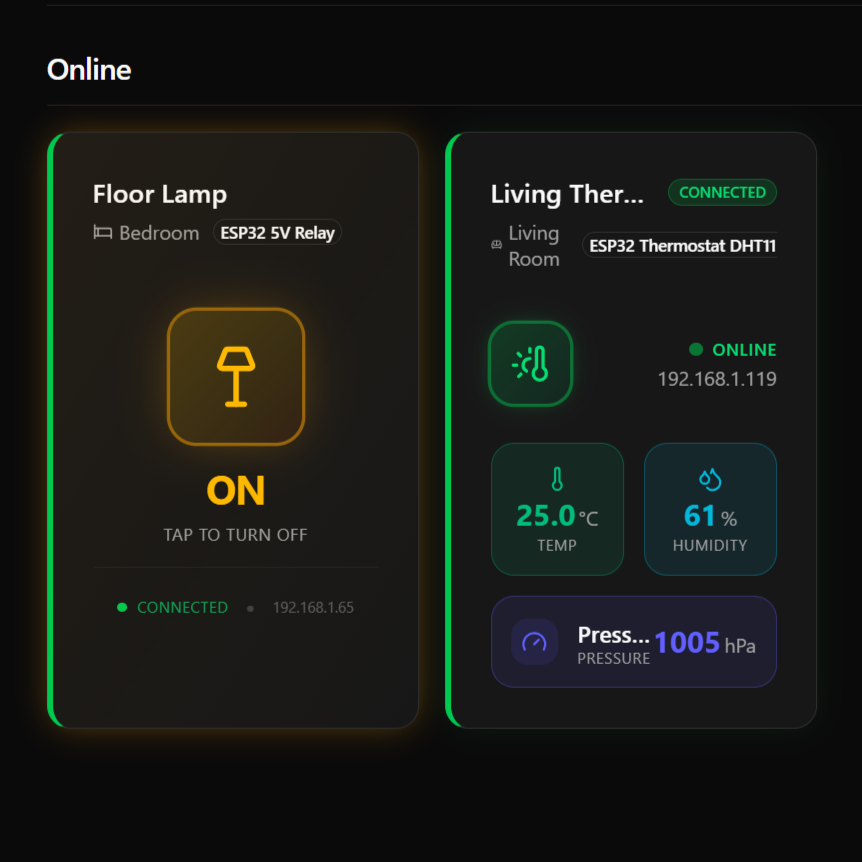
\includegraphics[width=0.95\textwidth]{figuri/test3_real_device.png}
    \caption{Testul 3: dispozitiv ESP32 real adăugat și controlat (screenshot de adăugat)}
    \label{fig:test3_real_device}
\end{figure}

\subsection{Test 4: detecția dispozitivelor offline}
\begin{enumerate}
    \item alimentarea ESP32-ului pornită, dispozitivul este \emph{online};
    \item dezalimentarea ESP32-ului;
    \item urmărirea log-urilor backend-ului: după aproximativ 30 de secunde, \texttt{mqtt\_listener.check\_offline\_devices()} marchează dispozitivul ca \texttt{offline} și apare mesajul \emph{Device <nume> timed out. Marking OFFLINE.};
    \item în UI, cardul devine gri-decolorat și toggle-ul este dezactivat;
    \item realimentarea ESP32 — în maxim 5 secunde, primul \texttt{publishState()} aduce dispozitivul înapoi la \emph{online}.
\end{enumerate}

\subsection{Test 5: persistența layout-ului dashboard-ului}
\begin{enumerate}
    \item în modul edit, rearanjarea cardurilor, crearea unui folder cu 3 dispozitive;
    \item ieșirea din modul edit — \texttt{flushSave} forțează un \texttt{PUT /api/dashboard-layout/} imediat (vezi \texttt{useDashboardLayout.ts:89-98});
    \item refresh hard de browser (\texttt{Ctrl+Shift+R}) — layout-ul revine identic;
    \item ștergerea cookie-urilor și \texttt{localStorage}-ului, urmată de re-login — layout-ul este încă acolo (pentru că este servit de pe server, nu doar din \texttt{localStorage}).
\end{enumerate}

\subsection{Sinteza rezultatelor}
Tabelul \ref{tab:rezultate_teste} sumarizează observațiile pe cele cinci scenarii descrise mai sus. Toate testele au fost executate pe o mașină Linux Mint 22 (kernel 6.5) cu Docker 26.0, un ESP32 DevKit V1 conectat la rețeaua locală \texttt{192.168.1.0/24} și browserul Chromium 124.

\begin{table}[htbp]
    \centering
    \caption{Rezultatele celor cinci scenarii de testare manuală}
    \label{tab:rezultate_teste}
    \renewcommand{\arraystretch}{1.3}
    \footnotesize
    \begin{tabular}{|p{1cm}|p{3.5cm}|p{4.2cm}|p{4.5cm}|}
        \hline
        \textbf{Nr.} & \textbf{Scenariu} & \textbf{Rezultat așteptat} & \textbf{Rezultat observat} \\ \hline
        1 & Primul utilizator $\rightarrow$ Owner & \texttt{role = owner}, \texttt{is\_superuser = True} & Confirmat — wizard $\rightarrow$ Settings arată badge \emph{Owner} \\ \hline
        2 & Propunere $\rightarrow$ Approve & Tipul apare în \emph{Device Types}, notificare la propunător & Confirmat — notificarea ajunge în mai puțin de 1 s în \emph{notification-center} \\ \hline
        3 & ESP32 real conectat & MAC bind automat, comandă $\rightarrow$ releu & Comandă executată în \textasciitilde 80 ms pe LAN (mediană pe 10 încercări) \\ \hline
        4 & Detecția offline & Status \texttt{offline} după 30 s & Confirmat — observat în \textasciitilde 32 s în medie \\ \hline
        5 & Layout persistent & Folder + ordine reluate la re-login & Confirmat pe Chromium, Firefox, Safari \\ \hline
    \end{tabular}
\end{table}

\section{Discuție: limitări și considerente de securitate}
Stack-ul actual este suficient pentru un mediu de laborator sau pentru o rețea casnică privată. Pentru un deployment în producție, există însă câteva îmbunătățiri necesare:
\begin{itemize}
    \item \textbf{TLS pe broker.} \texttt{allow\_anonymous true} este acceptabil doar într-un LAN izolat; pentru un mediu real, ar trebui generate certificate (\texttt{mosquitto\_passwd}) și configurate ACL-uri (\texttt{aclfile}) per topic.
    \item \textbf{Politica de parolă.} Cerința actuală de minimum 4 caractere este deliberat permisivă pentru un mediu de demonstrație; o instalare de producție ar utiliza \texttt{MinimumLengthValidator(min\_length=12)} împreună cu o bibliotecă de \emph{breach detection}.
    \item \textbf{SECRET\_KEY și DEBUG.} Fișierul \texttt{settings.py} conține valori statice pentru \texttt{SECRET\_KEY} și \texttt{DEBUG = True}, ambele marcate explicit prin comentarii. Pentru deployment-ul în producție, este obligatorie transferarea lor în variabile de mediu și dezactivarea \texttt{DEBUG}.
    \item \textbf{CORS.} Setarea \texttt{CORS\_ALLOW\_ALL\_ORIGINS = True} este orientată către simplitatea dezvoltării; în producție, lista originilor permise trebuie restrânsă la domeniul instanței.
\end{itemize}
Modificările enumerate au un impact redus asupra codului, însă diferențiază clar un mediu didactic de unul de producție. În contextul prezentei lucrări, configurația a fost menținută în varianta permisivă pentru a permite ca obiectul principal al expunerii să rămână arhitectura platformei.

\chapter{Concluzii și direcții viitoare}

\section{Rezumatul lucrării}
Lucrarea a descris proiectarea și implementarea platformei HomeForge, un sistem Smart Home cu execuție locală, conceput simultan ca aplicație funcțională și ca material didactic. Spre deosebire de soluțiile comerciale dependente de servicii cloud sau de platformele open-source mature precum Home Assistant — caracterizate de un nivel ridicat de abstractizare care reduce accesibilitatea componentelor interne pentru un dezvoltator în formare — HomeForge menține o stivă tehnologică redusă și un flux de date observabil end-to-end.

Obiectivele declarate în Capitolul 1 au fost atinse după cum urmează:
\begin{itemize}
    \item \textbf{Firmware ESP32} modular, cu patru variante template (releu, termostat cu DHT11, termostat cu BMP180, variantă combinată) și un protocol de comunicație simplu peste MQTT, descris în Capitolul 5.
    \item \textbf{Backend Django} cu un API REST complet, autentificare bazată pe JWT, sistem ierarhic de roluri \texttt{owner/admin/user} și un proces MQTT dedicat care leagă stratul hardware de baza de date PostgreSQL (Capitolul 3).
    \item \textbf{Frontend Next.js} cu dashboard interactiv, mecanism de optimistic UI pe carduri, layout persistat pe server, editor vizual pentru tipuri de dispozitive și vizualizare a topologiei prin React Flow (Capitolul 4).
    \item \textbf{Deployment containerizat} printr-o singură comandă \texttt{docker compose up}, completat cu un mod de dezvoltare nativ (Capitolul 6).
\end{itemize}

\section{Contribuții proprii}
La nivel cantitativ, contribuția proprie acoperă întreaga stivă: aproximativ 2500 de linii de Python pentru backend (\texttt{api/}), peste 12000 de linii TypeScript și JavaScript pentru frontend (\texttt{frontend/}) și cele patru proiecte de firmware ESP32 (circa 200 de linii fiecare). Pe lângă volumul de cod, câteva elemente arhitecturale particulare reprezintă contribuții substanțiale ale acestei lucrări:

\begin{enumerate}
    \item \textbf{Stocare schema-less peste RDBMS.} Starea fiecărui dispozitiv este stocată într-un \texttt{JSONField} mapat pe tipul nativ \texttt{JSONB} din PostgreSQL, în timp ce relațiile structurale (utilizator, cameră, tip de dispozitiv) rămân normalizate. Adăugarea unui nou tip de senzor nu necesită migrații SQL, iar mecanismele de control al accesului se sprijină în continuare pe integritatea referențială a schemei relaționale.
    \item \textbf{Auto-binding MAC--IP.} Mecanismul prin care procesul \texttt{mqtt\_listener} asociază automat un dispozitiv recent înregistrat (cunoscut inițial doar prin adresa IP) cu prima publicare MQTT, care conține adresa MAC. Astfel, utilizatorul nu trebuie să introducă manual adresa MAC, eliminând o sursă frecventă de erori.
    \item \textbf{Mapare „chei standard $\rightarrow$ identificatori widget".} Firmware-ul publică datele sub denumiri canonice (\texttt{temperature}, \texttt{humidity}, \texttt{relay\_1}), iar procesul de ascultare le traduce în identificatorii dinamici generați de \emph{device builder}. Drept consecință, reorganizarea widget-urilor pe card nu impune reflash-area firmware-ului.
    \item \textbf{Optimistic UI cu rollback.} Implementarea cardurilor inteligente prin \texttt{onMutate}, \texttt{onError} și \texttt{onSettled} din TanStack Query, în corespondență cu răspunsul \texttt{HTTP 202 Accepted} din backend, oferă feedback vizual imediat și revine corect la starea anterioară în cazul în care dispozitivul nu confirmă comanda. Mecanismul \texttt{matchesOptimistic} elimină situațiile în care interfața ar rămâne blocată în starea de sincronizare.
    \item \textbf{Device builder vizual.} Editorul bazat pe un graf de noduri și un panou de widget-uri, dublat de o validare server-side care impune ca fiecare \texttt{variable\_mapping} să corespundă unui ID definit în \texttt{structure[]}, permite contribuția unor tipuri noi de dispozitive fără modificări la nivelul codului platformei.
    \item \textbf{Layout cu cascadă de fallback.} Mecanismul ierarhic \emph{layout personal $\rightarrow$ layout partajat de administrator $\rightarrow$ implicit calculat client-side} permite administratorilor să stabilească o configurație inițială pentru utilizatorii noi, fără a restricționa personalizarea ulterioară a fiecăruia.
\end{enumerate}

\section{Limitări cunoscute}
Versiunea actuală a platformei prezintă o serie de limitări care trebuie semnalate explicit.

\paragraph{Securitate.} După cum s-a detaliat în Capitolul 6, brokerul Mosquitto este configurat cu \texttt{allow\_anonymous true}, comunicarea MQTT nu folosește TLS, iar variabilele Django sensibile (\texttt{SECRET\_KEY}, \texttt{DEBUG}) au valori statice. Aceste setări sunt acceptabile pentru un mediu de laborator, dar nu și pentru o instanță expusă în internet.

\paragraph{Lipsa OTA și a captive portal-ului.} Reconfigurarea sau actualizarea unui ESP32 presupune conectarea fizică prin USB. O versiune ulterioară ar putea integra ArduinoOTA sau ESPHome pentru actualizări la distanță.

\paragraph{Scalabilitate.} Cache-urile sunt locale (\texttt{LocMemCache} din Django), brokerul Mosquitto rulează în același container cu Django, iar baza de date este unică. Limita practică a implementării curente este de ordinul a câteva sute de dispozitive simultan, ceea ce acoperă scenariile rezidențiale, dar nu și pe cele de scară superioară.

\paragraph{Absența automatizărilor.} HomeForge expune dispozitivele și permite controlul manual, dar nu include încă un motor de reguli de tip \emph{trigger $\rightarrow$ condition $\rightarrow$ action}, cum oferă Home Assistant. Adăugarea acestuia constituie o direcție evidentă de continuare.

\paragraph{Testare automată.} Repository-ul conține fișierul \texttt{tests.py}, dar acoperirea testelor unitare și de integrare rămâne modestă. O eventuală evoluție către un proiect mentenabil pe termen lung impune extinderea suitei pentru a acoperi serializerele principale, fluxurile RBAC și mecanismele din \texttt{mqtt\_listener}.

\section{Direcții viitoare}
Pe baza limitărilor identificate, se pot evidenția cinci direcții de dezvoltare ulterioară.

\begin{enumerate}
    \item \textbf{TLS și autentificare MQTT.} Configurarea Mosquitto cu certificate generate automat, integrate într-un asistent de inițializare. Firmware-ul ar putea utiliza \texttt{WiFiClientSecure} cu un \texttt{rootCA} predefinit.
    \item \textbf{Motor de automatizări.} Un model Django \texttt{Automation} cu câmpurile \texttt{trigger\_topic}, \texttt{condition\_expr}, \texttt{action\_topic} și \texttt{action\_payload}, evaluat de un proces care ascultă același flux MQTT ca \texttt{mqtt\_listener}. Pe frontend, un editor vizual analog cu device builder-ul.
    \item \textbf{Suport pentru protocoale suplimentare.} Adăugarea unui adaptor pentru \texttt{Matter} sau \texttt{Zigbee2MQTT} ar permite integrarea dispozitivelor comerciale, fără abandonarea principiului \emph{local-first}. Adaptoarele ar publica pe aceleași topice \texttt{homeforge/devices/...}, astfel încât restul stivei să rămână nemodificat.
    \item \textbf{Mod public read-only.} Posibilitatea expunerii unei pagini publice (semnată cu un token) care să prezinte un subset de dispozitive în regim read-only, utilă pentru monitorizare la distanță fără a expune întreaga aplicație.
    \item \textbf{Pipeline CI/CD.} Un flux GitHub Actions care să ruleze \texttt{python manage.py test}, \texttt{npm run build} și \texttt{eslint} la fiecare \emph{pull request}, completat cu construirea imaginilor Docker la fiecare tag.
\end{enumerate}

\section{Învățări personale}
Implementarea acestei platforme a oferit ocazia parcurgerii practice a etapelor de cuplare între o stivă web modernă și un strat embedded. Patru observații se desprind ca fiind relevante pentru proiecte similare. Prima: definirea precisă a contractelor de date este mai importantă decât alegerea unui protocol anume — dezbaterea „REST vs. MQTT vs. WebSocket" devine secundară odată ce este clar ce informație circulă între componente. A doua: optimistic UI nu este o decorație vizuală, ci o strategie de gestiune a timpului perceput de utilizator, iar un mecanism de rollback robust este la fel de important ca redarea instantanee inițială. A treia: transparența arhitecturală generează un cost de implementare, dar simplifică considerabil etapa de depanare — observarea directă a traficului MQTT cu \texttt{mosquitto\_sub} s-a dovedit utilă în mod repetat. A patra: o bază de date relațională extinsă cu \texttt{JSONB} reprezintă, în numeroase scenarii, o alternativă preferabilă unei baze NoSQL pure, oferind flexibilitate fără pierderea garanțiilor ACID sau a ergonomiei unui ORM matur.

\section{Reflecție finală}
HomeForge nu își propune să acopere integralitatea funcționalităților unei platforme Smart Home comerciale. Rolul său este intermediar: face legătura între noțiunile teoretice predate la cursurile de rețele, sisteme distribuite și baze de date și aplicarea lor concretă într-un sistem care interacționează cu mediul fizic. Considerând obiectivul didactic, lucrarea poate fi utilă oricărui student sau dezvoltator care dorește să își configureze un ESP32 propriu și să urmărească, linie cu linie, traseul unei valori senzoriale de la dispozitiv până la dashboard.

Codul sursă rămâne disponibil în repository-ul proiectului, deschis utilizării, modificării și extinderii ulterioare în contextul educațional și academic.


% \nocite{*}
% Bibliografia se afișează cu spațiere simplă, conform cerințelor UPB
% (în teza-upb.cls, mediul \thebibliography setează \baselinestretch{1};
% biblatex are propriul mediu, deci aplicăm setarea explicit).
{\singlespacing
\printbibliography[heading=bibintoc,title={Bibliografie}]
}

\appendix

\chapter{Backend}

\section{Modelele de date (\texttt{api/\allowbreak models.py})}
\label{anexa:models}
\inputminted{python}{cod/models.py}

\section{Serializere și validare (\texttt{api/\allowbreak serializers.py})}
\label{anexa:serializers}
\inputminted{python}{cod/serializers.py}

\section{Permisiuni RBAC (\texttt{api/\allowbreak permissions.py})}
\label{anexa:permissions}
\inputminted{python}{cod/permissions.py}

\section{Daemonul MQTT (\texttt{api/\allowbreak management/\allowbreak commands/\allowbreak mqtt\_listener.py})}
\label{anexa:mqtt_listener}
\inputminted{python}{cod/mqtt_listener.py}

\section{Clientul MQTT de publicare (\texttt{api/\allowbreak mqtt\_client.py})}
\label{anexa:mqtt_client}
\inputminted{python}{cod/mqtt_client.py}

\section{Adaptorul Fronius pentru sisteme solare (\texttt{api/\allowbreak solar/\allowbreak providers/\allowbreak fronius.py})}
\label{anexa:fronius}
\inputminted{python}{cod/fronius.py}

\chapter{Frontend}

\section{Comunicarea cu API-ul și gestiunea JWT (\texttt{lib/\allowbreak apiClient.js})}
\label{anexa:apiclient}
\inputminted{javascript}{cod/apiClient.js}

\section{Cardul inteligent și optimistic UI (\texttt{components/\allowbreak devices/\allowbreak SmartDeviceCard.tsx})}
\label{anexa:smartdevicecard}
\inputminted{typescript}{cod/SmartDeviceCard.tsx}

\section{Hook-ul de layout al dashboard-ului (\texttt{hooks/\allowbreak useDashboardLayout.ts})}
\label{anexa:dashboardlayout}
\inputminted{typescript}{cod/useDashboardLayout.ts}

\section{Editorul vizual de tipuri de dispozitive (\texttt{device-builder/\allowbreak DeviceUICreator.tsx})}
\label{anexa:deviceuicreator}
\inputminted{typescript}{cod/DeviceUICreator.tsx}


\end{document}
